        %%******************************************%%
        %%                                          %%
        %%        Modello di tesi di laurea         %%
        %%            di Andrea Giraldin            %%
        %%                                          %%
        %%             2 novembre 2012              %%
        %%                                          %%
        %%******************************************%%


% I seguenti commenti speciali impostano:
% 1. 
% 2. PDFLaTeX come motore di composizione;
% 3. tesi.tex come documento principale;
% 4. il controllo ortografico italiano per l'editor.

% !TEX encoding = UTF-8
% !TEX TS-program = pdflatex
% !TEX root = tesi.tex
% !TEX spellcheck = it-IT

\documentclass[10pt,                    % corpo del font principale
               a4paper,                 % carta A4
               twoside,                 % impagina per fronte-retro
               openright,               % inizio capitoli a destra
               english,                 
               italian,                 
               ]{book}    

%**************************************************************
% Importazione package
%************************************************************** 

%\usepackage{amsmath,amssymb,amsthm}    % matematica

\usepackage[T1]{fontenc}                % codifica dei font:
                                        % NOTA BENE! richiede una distribuzione *completa* di LaTeX

\usepackage[utf8]{inputenc}             % codifica di input; anche [latin1] va bene
                                        % NOTA BENE! va accordata con le preferenze dell'editor

\usepackage[english, italian]{babel}    % per scrivere in italiano e in inglese;
                                        % l'ultima lingua (l'italiano) risulta predefinita

\usepackage{bookmark}                   % segnalibri

\usepackage{caption}                    % didascalie

\usepackage{chngpage,calc}              % centra il frontespizio

\usepackage{csquotes}                   % gestisce automaticamente i caratteri (")

\usepackage{emptypage}                  % pagine vuote senza testatina e piede di pagina

\usepackage{epigraph}			% per epigrafi

\usepackage{eurosym}                    % simbolo dell'euro

%\usepackage{indentfirst}               % rientra il primo paragrafo di ogni sezione

\usepackage{graphicx}                   % immagini

\usepackage{hyperref}                   % collegamenti ipertestuali

\usepackage[binding=5mm]{layaureo}      % margini ottimizzati per l'A4; rilegatura di 5 mm

\usepackage{listings}                   % codici

\usepackage{microtype}                  % microtipografia

\usepackage{mparhack,fixltx2e,relsize}  % finezze tipografiche

\usepackage{nameref}                    % visualizza nome dei riferimenti                                      

\usepackage[font=small]{quoting}        % citazioni

\usepackage{subfig}                     % sottofigure, sottotabelle

\usepackage[italian]{varioref}          % riferimenti completi della pagina

\usepackage[dvipsnames]{xcolor}         % colori

\usepackage{booktabs}                   % tabelle                                       
\usepackage{tabularx}                   % tabelle di larghezza prefissata                                    
\usepackage{longtable}                  % tabelle su più pagine                                        
\usepackage{ltxtable}                   % tabelle su più pagine e adattabili in larghezza

\usepackage[toc, acronym]{glossaries}   % glossario
                                        % per includerlo nel documento bisogna:
                                        % 1. compilare una prima volta tesi.tex;
                                        % 2. eseguire: makeindex -s tesi.ist -t tesi.glg -o tesi.gls tesi.glo
                                        % 3. eseguire: makeindex -s tesi.ist -t tesi.alg -o tesi.acr tesi.acn
                                        % 4. compilare due volte tesi.tex.

\usepackage[backend=bibtex,hyperref,backref]{biblatex}
                                        % eccellente pacchetto per la bibliografia; 
                                        % produce uno stile di citazione autore-anno; 
                                        % lo stile "numeric-comp" produce riferimenti numerici
                                        % per includerlo nel documento bisogna:
                                        % 1. compilare una prima volta tesi.tex;
                                        % 2. eseguire: biber tesi
                                        % 3. compilare ancora tesi.tex.

%**************************************************************
% file contenente le impostazioni della tesi
%**************************************************************

%**************************************************************
% Frontespizio
%**************************************************************

% Autore
\newcommand{\myName}{Marco Pozza}
\newcommand{\myTitle}{Identity Trust Fabric: sistema per la gestione dell'identità e l'accesso ai servizi basato su Blockchain}

% Tipo di tesi                   
\newcommand{\myDegree}{Tesi di laurea triennale}

% Università             
\newcommand{\myUni}{Università degli Studi di Padova}

% Facoltà       
\newcommand{\myFaculty}{Corso di Laurea in Informatica}

% Dipartimento
\newcommand{\myDepartment}{Dipartimento di Matematica "Tullio Levi-Civita"}

% Titolo del relatore
\newcommand{\profTitle}{Prof.}

% Relatore
\newcommand{\myProf}{Luigi De Giovanni}

% Luogo
\newcommand{\myLocation}{Padova}

% Anno accademico
\newcommand{\myAA}{2017-2018}

% Data discussione
\newcommand{\myTime}{Settembre 2018}


%**************************************************************
% Impostazioni di impaginazione
% see: http://wwwcdf.pd.infn.it/AppuntiLinux/a2547.htm
%**************************************************************

\setlength{\parindent}{14pt}   % larghezza rientro della prima riga
\setlength{\parskip}{0pt}   % distanza tra i paragrafi


%**************************************************************
% Impostazioni di biblatex
%**************************************************************
\bibliography{bibliografia} % database di biblatex 

\defbibheading{bibliography} {
    \cleardoublepage
    \phantomsection 
    \addcontentsline{toc}{chapter}{\bibname}
    \chapter*{\bibname\markboth{\bibname}{\bibname}}
}

\setlength\bibitemsep{1.5\itemsep} % spazio tra entry

\DeclareBibliographyCategory{opere}
\DeclareBibliographyCategory{web}

\addtocategory{opere}{womak:lean-thinking}
\addtocategory{web}{site:agile-manifesto}

\defbibheading{opere}{\section*{Riferimenti bibliografici}}
\defbibheading{web}{\section*{Siti Web consultati}}


%**************************************************************
% Impostazioni di caption
%**************************************************************
\captionsetup{
    tableposition=top,
    figureposition=bottom,
    font=small,
    format=hang,
    labelfont=bf
}

%**************************************************************
% Impostazioni di glossaries
%**************************************************************

%**************************************************************
% Acronimi
%**************************************************************
\renewcommand{\acronymname}{Acronimi e abbreviazioni}
%\newacronym[description={\glslink{ITF}{Identity Trust Fabric}}]{ITF}{Identity Trust Fabric}
\newacronym{ITF}{ITF}{Identity Trust Fabric}

%**************************************************************
% Glossario
%**************************************************************
%\renewcommand{\glossaryname}{Glossario}
%\newglossaryentry{umlg}
%{
%	name=\glslink{uml}{UML},
%	text=UML,
%	sort=uml,
%	description={in ingegneria del software \emph{UML, Unified Modeling Language} (ing. linguaggio di modellazione unificato) è un linguaggio di modellazione e specifica basato sul paradigma object-oriented. L'\emph{UML} svolge un'importantissima funzione di ``lingua franca'' nella comunità della progettazione e programmazione a oggetti. Gran parte della letteratura di settore usa tale linguaggio per descrivere soluzioni analitiche e progettuali in modo sintetico e comprensibile a un vasto pubblico}
%}
\newglossaryentry{agile}
{
	name=Agile,
	description={
		 In ingegneria del software, è un insieme di metodi di sviluppo del software emersi a partire dai primi anni 2000 e fondati su un insieme di principi comuni, direttamente o indirettamente derivati dai principi del \textit{Manifesto per lo sviluppo agile del software}\cite{manifestoAgile}.\\
		 Tale manifesto si può riassumere in quattro punti:
		 \begin{enumerate}
		 	\item le persone e le interazioni sono più importanti dei processi e degli strumenti;
		 	\item è più importante avere software funzionante che documentazione
		 	\item bisogna collaborare con i clienti oltre che rispettare il contratto;
		 	\item bisogna essere pronti a rispodere ai cambiamenti oltre che aderire alla pianificazione.
		 \end{enumerate}
		 Un esempio di metodo di sviluppo di tipo agile è il metodo \gls{Scrum}}
}
\newglossaryentry{DataManagement}
{
	name=Data Management,
	description={insime di più attività che hanno lo scopo di sviluppare, eseguire e supervisionare progetti, politiche e programmi che controllano, proteggono, trasportano e aumentano il valore di dati e di risorse informative}
}
\newglossaryentry{DataMining}
{
  name=Data Mining,
  description={Insieme di tecniche e metodologie che hanno per oggetto l'estrazione di informazioni da grandi quantità di dati attraverso
  emtodi automatici o semi-automatici}
}
\newglossaryentry{Scrum}
{
	name=Scrum,
	description={Metodo di sviluppo software che rientra fra i metodi agile. Prevede di dividere il progetto in blocchi rapidi di lavoro (\textit{sprint}) alla fine di ciascuno dei quali crea un incremento del software. Esso indica come definire i dettagli del lavoro da fare nell'immediato futuro e prevede vari meeting con caratteristiche precise per creare occasioni di ispezione e controllo del lavoro svolto \cite{scrum}
	}
}
\newglossaryentry{ProductBacklog}
{
	name= Product Backlog,
	description={Insime di requisiti per il lavoro da compiere, con priorità assegnate in base al valore di business}
}
\newglossaryentry{SprintBacklog}
{
	name= Sprint Backlog,
	description={Insieme degli elementi selezionati dal Product Backlog per lo \textit{sprint}}
}
\newglossaryentry{IAM}
{
	name=Identity and Access Management,
	description={L'Identity and Access Management è un sistema che si occupa della gestione delle informazioni riguardanti l'identità degli utenti e controlla l'accesso alle risorse informatiche. Nello specifico:
	\begin{itemize}
		\item \textbf{Identity Management} - censisce le utenze;
		\item \textbf{Access Management} - gestisce l'autenticazione e l'autorizzazione delle utenze. 
	\end{itemize}}
}
\newglossaryentry{identityWallet}{
	name=Identity Wallet,
	description={Portafogli digitali che contengono all'loro interno tutte le informazioni necessarie ad un utente per poter permettere l'autenticazione preciso servizio}
}
\newglossaryentry{monokee}{
name = Monokee,
description={Un \emph{\gls{IaaS}}\glsfirstoccur ideato e sviluppato da Athesys S.r.l per realizzare l'\gls{IAM}}
}
\newglossaryentry{IaaS}{
	name =Identity-as-a-Service,
	description ={È un servizio cloud che fornisce funzionalità di Identity and Access Management ad un sistema nel cloud e/o locale}
}
\newglossaryentry{identityProofing}{
	name=Identity Proofing,
	description={Conosciuta anche come \textit{Identity Verification} significa verificare ed autenticare l'identità di un utente prima che questo possa avere accesso ad uno o più servizi}
}
\newglossaryentry{identityBinding}{
	name=Identity Binding,
	description={Legare l'identità digitale all'individuo che la reclama attraverso vari meccanismi di riconoscimento che possono cambiare a seconda dell'ente di emissione dell'identità digitale stessa}
}
\newglossaryentry{designPatterns}{
name=Design Patterns,
description={Legare l'identità digitale all'individuo che la reclama attraverso vari meccanismi di riconoscimento che possono cambiare a seconda dell'ente di emissione dell'identità digitale stessa}
}
\newglossaryentry{poc}{
	name=Proof of Concept,
	description={si può tradurre in italiano con prova di concetto, si intende un'incompleta realizzazione o abbozzo di un certo progetto o metodo, con lo scopo di dimostrarne la fattibilità o la fondatezza di alcuni principi o concetti costituenti.}
}
\newglossaryentry{dlt}{
	name=Distributed Ledger,
	description={viene chiamato anche Registro Distribuito. Sono dei database distribuiti, ovvero di Ledgers (Libri Mastro) che possono essere aggiornati, gestiti, controllati e coordinati non più solo a livello centrale, ma in modo distribuito, da parte di tutti gli attori.}
}
\newglossaryentry{pow}{
	name=Proof of Work,
	description={metodologia utilizzata dalle \textit{Blockchain} per impedire attacchi di tipo Denial of Service o spam nella rete. Questo metodo di prevenzione richiede la risoluzione di un complesso gioco matematico la cui risoluzione fa si che il blocco sia inserito nella \textit{Blockchain}\cite{proof_of_work}}
}
\newglossaryentry{dos}{
	name=Denial of Service,
	description={attacco informatico in cui si fanno esaurire deliberatamente le risorse di un sistema informatico che fornisce un servizio ai client, fino a renderlo non più in grado di erogare il servizio richiesto\cite{Denial_of_service}}
}

 % database di termini
\makeglossaries


%**************************************************************
% Impostazioni di graphicx
%**************************************************************
\graphicspath{{immagini/}} % cartella dove sono riposte le immagini


%**************************************************************
% Impostazioni di hyperref
%**************************************************************
\hypersetup{
    %hyperfootnotes=false,
    %pdfpagelabels,
    %draft,	% = elimina tutti i link (utile per stampe in bianco e nero)
    colorlinks=true,
    linktocpage=true,
    pdfstartpage=1,
    pdfstartview=FitV,
    % decommenta la riga seguente per avere link in nero (per esempio per la stampa in bianco e nero)
    %colorlinks=false, linktocpage=false, pdfborder={0 0 0}, pdfstartpage=1, pdfstartview=FitV,
    breaklinks=true,
    pdfpagemode=UseNone,
    pageanchor=true,
    pdfpagemode=UseOutlines,
    plainpages=false,
    bookmarksnumbered,
    bookmarksopen=true,
    bookmarksopenlevel=1,
    hypertexnames=true,
    pdfhighlight=/O,
    %nesting=true,
    %frenchlinks,
    urlcolor=webbrown,
    linkcolor=RoyalBlue,
    citecolor=webgreen,
    %pagecolor=RoyalBlue,
    %urlcolor=Black, linkcolor=Black, citecolor=Black, %pagecolor=Black,
    pdftitle={\myTitle},
    pdfauthor={\textcopyright\ \myName, \myUni, \myFaculty},
    pdfsubject={},
    pdfkeywords={},
    pdfcreator={pdfLaTeX},
    pdfproducer={LaTeX}
}

%**************************************************************
% Impostazioni di itemize
%**************************************************************
\renewcommand{\labelitemi}{$\ast$}

%\renewcommand{\labelitemi}{$\bullet$}
%\renewcommand{\labelitemii}{$\cdot$}
%\renewcommand{\labelitemiii}{$\diamond$}
%\renewcommand{\labelitemiv}{$\ast$}


%**************************************************************
% Impostazioni di listings
%**************************************************************
\lstset{
    language=[LaTeX]Tex,%C++,
    keywordstyle=\color{RoyalBlue}, %\bfseries,
    basicstyle=\small\ttfamily,
    %identifierstyle=\color{NavyBlue},
    commentstyle=\color{Green}\ttfamily,
    stringstyle=\rmfamily,
    numbers=none, %left,%
    numberstyle=\scriptsize, %\tiny
    stepnumber=5,
    numbersep=8pt,
    showstringspaces=false,
    breaklines=true,
    frameround=ftff,
    frame=single
} 


%**************************************************************
% Impostazioni di xcolor
%**************************************************************
\definecolor{webgreen}{rgb}{0,.5,0}
\definecolor{webbrown}{rgb}{.6,0,0}


%**************************************************************
% Altro
%**************************************************************

\newcommand{\omissis}{[\dots\negthinspace]} % produce [...]

% eccezioni all'algoritmo di sillabazione
\hyphenation
{
    ma-cro-istru-zio-ne
    gi-ral-din
}

\newcommand{\sectionname}{sezione}
\addto\captionsitalian{\renewcommand{\figurename}{Figura}
                       \renewcommand{\tablename}{Tabella}}

\newcommand{\glsfirstoccur}{\ap{{[g]}}}

\newcommand{\intro}[1]{\emph{\textsf{#1}}}

%**************************************************************
% Environment per ``rischi''
%**************************************************************
\newcounter{riskcounter}                % define a counter
\setcounter{riskcounter}{0}             % set the counter to some initial value

%%%% Parameters
% #1: Title
\newenvironment{risk}[1]{
    \refstepcounter{riskcounter}        % increment counter
    \par \noindent                      % start new paragraph
    \textbf{\arabic{riskcounter}. #1}   % display the title before the 
                                        % content of the environment is displayed 
}{
    \par\medskip
}

\newcommand{\riskname}{Rischio}

\newcommand{\riskdescription}[1]{\textbf{\\Descrizione:} #1.}

\newcommand{\risksolution}[1]{\textbf{\\Soluzione:} #1.}

%**************************************************************
% Environment per ``use case''
%**************************************************************
\newcounter{usecasecounter}             % define a counter
\setcounter{usecasecounter}{0}          % set the counter to some initial value

%%%% Parameters
% #1: ID
% #2: Nome
\newenvironment{usecase}[2]{
    \renewcommand{\theusecasecounter}{\usecasename #1}  % this is where the display of 
                                                        % the counter is overwritten/modified
    \refstepcounter{usecasecounter}             % increment counter
    \vspace{10pt}
    \par \noindent                              % start new paragraph
    {\large \textbf{\usecasename #1: #2}}       % display the title before the 
                                                % content of the environment is displayed 
    \medskip
}{
    \medskip
}

\newcommand{\usecasename}{UC}

\newcommand{\usecaseactors}[1]{\textbf{\\Attori Principali:} #1. \vspace{4pt}}
\newcommand{\usecasepre}[1]{\textbf{\\Precondizioni:} #1. \vspace{4pt}}
\newcommand{\usecasedesc}[1]{\textbf{\\Descrizione:} #1. \vspace{4pt}}
\newcommand{\usecasepost}[1]{\textbf{\\Postcondizioni:} #1. \vspace{4pt}}
\newcommand{\usecasealt}[1]{\textbf{\\Scenario Alternativo:} #1. \vspace{4pt}}

%**************************************************************
% Environment per ``namespace description''
%**************************************************************

\newenvironment{namespacedesc}{
    \vspace{10pt}
    \par \noindent                              % start new paragraph
    \begin{description} 
}{
    \end{description}
    \medskip
}

\newcommand{\classdesc}[2]{\item[\textbf{#1:}] #2}                     % file con le impostazioni personali

\usepackage{lmodern}

\begin{document}
%**************************************************************
% Materiale iniziale
%**************************************************************
\frontmatter
% !TEX encoding = UTF-8
% !TEX TS-program = pdflatex
% !TEX root = ../tesi.tex

%**************************************************************
% Frontespizio 
%**************************************************************
\begin{titlepage}

\begin{center}

\begin{LARGE}
\textbf{\myUni}\\
\end{LARGE}

\vspace{10pt}

\begin{Large}
\textsc{\myDepartment}\\
\end{Large}

\vspace{10pt}

\begin{large}
\textsc{\myFaculty}\\
\end{large}

\vspace{30pt}
\begin{figure}[htbp]
\begin{center}

\includegraphics[height=6cm]{logo-unipd}
\end{center}
\end{figure}
\vspace{30pt} 

\begin{LARGE}
\begin{center}
\textbf{\myTitle}\\
\end{center}
\end{LARGE}

\vspace{10pt} 

\begin{large}
\textsl{\myDegree}\\
\end{large}

\vspace{40pt} 

\begin{large}
\begin{flushleft}
\textit{Relatore}\\ 
\vspace{5pt} 
\profTitle \myProf
\end{flushleft}

\vspace{0pt} 

\begin{flushright}
\textit{Laureando}\\ 
\vspace{5pt} 
\myName
\end{flushright}
\end{large}

\vspace{20pt}

\line(1, 0){338} \\
\begin{normalsize}
\textsc{Anno Accademico \myAA}
\end{normalsize}

\end{center}
\end{titlepage} 
% !TEX encoding = UTF-8
% !TEX TS-program = pdflatex
% !TEX root = ../tesi.tex

%**************************************************************
% Colophon
%**************************************************************
\clearpage
\phantomsection
\thispagestyle{empty}

\hfill

\vfill

\noindent\myName: \textit{\myTitle,}
\myDegree,
\textcopyright\ \myTime.
% !TEX encoding = UTF-8
% !TEX TS-program = pdflatex
% !TEX root = ../tesi.tex

%**************************************************************
% Dedica
%**************************************************************
\cleardoublepage
\phantomsection
\thispagestyle{empty}
\pdfbookmark{Dedica}{Dedica}

\vspace*{3cm}

\begin{center}
 Anche un viaggio di mille miglia inizia con un passo. \\ \medskip
--- Confucio    
\end{center}

\medskip

\begin{center}
A mio nonno Mario che, nonostante non possa vedermi crescere, spero sia fiero dell'uomo che sto diventando.
\end{center}

% !TEX encoding = UTF-8
% !TEX TS-program = pdflatex
% !TEX root = ../tesi.tex

%**************************************************************
% Sommario
%**************************************************************
\cleardoublepage
\phantomsection
\pdfbookmark{Sommario}{Sommario}
\begingroup
\let\clearpage\relax
\let\cleardoublepage\relax
\let\cleardoublepage\relax

\chapter*{Sommario}

Il presente documento descrive il lavoro svolto duarante il periodo di stage, della durata di circa trecentoventi ore, del lauraendo Marco Pozza presso l'azienda Athesys S.r.l di Padova.\\\\
Lo scopo principale dello stage consistenva nella realizzazione di un layer di sicurezza, denominato Identity Trust Fabric (ITF) per integrare una tecnologia blockchain nei processi di accesso ai servizi e condivisione degli attributi di profilo.\\\\
Inoltre era richiesto che tale modulo venisse integrato come estensione delle funzionalità di un prodotto di Identity and Access Management già utilizzato dall'azienda.\\\\
Gli obiettivi da raggiungere erano vari.\\
In primo luogo era richiesto lo studio di fattibilità, seguito da analisi dei requisiti e progettazione architetturale e di dettaglio dell'intero sistema.\\\\
In secondo luogo era richiesta l'implementazione del modulo ITF utilizzando gli strumenti e seguendo le specifiche individuate nel primo periodo di stage.\\\\
Terzo ed ultimo obiettivo era la codifica di test per accertare che il modulo codificato funzionasse correttamente.

%\vfill
%
%\selectlanguage{english}
%\pdfbookmark{Abstract}{Abstract}
%\chapter*{Abstract}
%
%\selectlanguage{italian}

\endgroup			

\vfill


% !TEX encoding = UTF-8
% !TEX TS-program = pdflatex
% !TEX root = ../tesi.tex

%**************************************************************
% Organizzazione del Testo
%**************************************************************
\cleardoublepage
\phantomsection
\pdfbookmark{Organizzazione del Testo}{Organizzazione del Testo}
\begingroup
\let\clearpage\relax
\let\cleardoublepage\relax
\let\cleardoublepage\relax

\chapter*{Organizzazione del Testo}

\begin{description}
	\item[{\hyperref[cap:introduzione]{Capitolo 1}}] descrive l'azienda e le sue metodologie di lavoro. Inoltre viene descritto, nel dettaglio, il progetto di stage partendo da una panoramica generale del problema fino ad arrivare alla descrizione delle sue possibili soluzioni. Vengono esposti, infine, gli obiettivi da raggiungere e la pianificazione iniziale.
	
	\item[{\hyperref[cap:tecnologie_e_strumenti]{Capitolo 2}}] fornisce una descrizione delle tecnologie individuate e, dopo un dettagliato confronto, fornisce una panoramica di tutti gli strumenti utilizzati per l'implementazione,la deploy ed il testing del modulo ITF. 
	
	\item[{\hyperref[cap:analisi-requisiti]{Capitolo 3}}] formalizza tutti i casi d'uso e i requisiti raccolti in fase di analisi dei requisiti.
	
	\item[{\hyperref[cap:progettazione]{Capitolo 4}}] illustra in modo esaustitvo il Design Pattern architetturale e le scelte implementatitve adottate per la realizzazione del sistema.
	
	\item[{\hyperref[cap:codifica_e_verifia]{Capitolo 5}}] fornisce una visione degli aspetti inerenti la codifica, il modulo realizzato e le tecniche di verifica e validazione adottate.
	
	\item[{\hyperref[cap:analisi-requisiti]{Capitolo 6}}] fornisce una valutazione finale dello stage comprensiva degli obiettivi raggiunti, le conoscenze acquisite e le difficoltà riscontrate durante lo stage.
	
\end{description}

Riguardo la stesura del testo, relativamente al documento sono state adottate le seguenti convenzioni tipografiche:
\begin{itemize}
	\item gli acronimi, le abbreviazioni e i termini ambigui o di uso non comune menzionati vengono definiti nel glossario, situato alla fine del presente documento;
	\item per la prima occorrenza dei termini riportati nel glossario viene utilizzata la seguente nomenclatura: \emph{parola}\glsfirstoccur;
	\item i termini in lingua straniera o facenti parti del gergo tecnico sono evidenziati con il carattere \emph{corsivo}.
\end{itemize}

\endgroup			

\vfill
% !TEX encoding = UTF-8
% !TEX TS-program = pdflatex
% !TEX root = ../tesi.tex

%**************************************************************
% Ringraziamenti
%**************************************************************
\cleardoublepage
\phantomsection
\pdfbookmark{Ringraziamenti}{ringraziamenti}

%\begin{flushright}{
%	\slshape    
%	``Life is really simple, but we insist on making it complicated''} \\ 
%	\medskip
%    --- Confucius
%\end{flushright}


\bigskip

\begingroup
\let\clearpage\relax
\let\cleardoublepage\relax
\let\cleardoublepage\relax

\chapter*{Ringraziamenti}

\noindent \textit{Vorrei innanzitutto ringraziare il mio tutor aziendale, Sara Meneghetti, ed il responsabile, Roberto Griggio, per la fiducia e la responsabilità affidatami durante tutto il periodo di stage, per la disponibilità e pazienza nei momenti di stallo; vorrei ringraziare, inoltre, tutte le persone che lavorano ad Athesys S.r.l, che nei due mesi di stage mi hanno, da subito, messo a mio agio facendomi sentire parte integrante del gruppo di lavoro.}\\

\noindent \textit{Desidero ringraziare tutti i miei parenti che hanno creduto in me e mi hanno sostenuto per tutti questi anni, in particolare mia zia Alessandra e mia nonna Rosy che durante i momenti di sconforto mi hanno sempre spronato a non mollare e ad andare avanti nonostante le difficoltà che  incontrate lungo il mio percorso.}\\

\noindent \textit{Un immenso grazie alla mia ragazza Giulia con la quale ho condiviso questi anni di studi.\\
La ringrazio per l'immensa pazienza che ha avuto nei momenti di più difficili dove, mi rendo conto, di esser stato una persona insopportabile e grazie per essermi stata vicino nell'affrontare gli esami che per me erano come una montagna da scalare.}\\

\noindent \textit{Un altro doveroso grazie va ai miei amici per tutte le risate e tutti i momenti condivisi insieme. Nei sabati e nelle domeniche in cui ci ritrovavamo siete sempre stati in grado di farmi dimenticare, anche se per poco, di tutti gli obblighi e doveri che avevo, facendomi sfogare e riprendere.}\\

\noindent \textit{Il grazie più importante va ai miei genitori che hanno permesso, con grandi sforzi e sacrifici, questa Laurea, per aver sempre creduto in me e per avermi insegnato quei valori che mi hanno reso quello che sono adesso, la persona che ha raggiunto questo primo ma importantissimo traguardo.}

\bigskip

\noindent\textit{\myLocation, \myTime}
\hfill \myName

\endgroup


% !TEX encoding = UTF-8
% !TEX TS-program = pdflatex
% !TEX root = ../tesi.tex

%**************************************************************
% Indici
%**************************************************************
\cleardoublepage
\pdfbookmark{\contentsname}{tableofcontents}
\setcounter{tocdepth}{2}
\tableofcontents
%\markboth{\contentsname}{\contentsname} 
\clearpage

\begingroup 
    \let\clearpage\relax
    \let\cleardoublepage\relax
    \let\cleardoublepage\relax
    %*******************************************************
    % Elenco delle figure
    %*******************************************************    
    \phantomsection
    \pdfbookmark{\listfigurename}{lof}
    \listoffigures

    \vspace*{8ex}

    %*******************************************************
    % Elenco delle tabelle
    %*******************************************************
    \phantomsection
    \pdfbookmark{\listtablename}{lot}
    \listoftables
        
    \vspace*{8ex}
\endgroup

\cleardoublepage

\cleardoublepage

%**************************************************************
% Materiale principale
%**************************************************************
\mainmatter
% !TEX encoding = UTF-8
% !TEX TS-program = pdflatex
% !TEX root = ../tesi.tex

%**************************************************************
\chapter{Introduzione}
\label{cap:introduzione}
%**************************************************************
In questo capitolo viene presentata, brevemente, l'azienda e la metodologia di lavoro che utilizza per lo sviluppo dei suoi progetti.\\
Verrà successivamente illustrato, in modo dettagliato, il progetto affrontato durante il periodo di stage partendo da una visione generale del problema e arrivando alle possibili soluzioni studiate.

%**************************************************************
\section{L'azienda}
\subsection{Profilo aziendale}
Athesys nasce nel 2010 con sede a Padova dall'unione di professionisti IT che vantano una lunga esperienza in diversi ambiti tecnologici con l’obiettivo di mettere a fattor comune la loro competenza e tradurla nella capacità di erogare consulenza ad elevato contenuto tecnologico e progettuale a supporto delle complesse scelte strategiche che le aziende sono chiamate a prendere con sempre maggiore rapidità \cite{athesys}.\\
I settori in cui l'azienda si muove sono diversi:
\begin{itemize}
	\item \textit{Identity and Access Management} - propone, alle aziende clienti, soluzioni per effettuare il controllo degli accessi alle applicazioni aziendali e di gestire il ciclo di vita degli account applicativi;
	\item \textit{Database Management} - aiuta le aziende a progettare i database più adatti alle loro esigenze focalizzandosi sull'alta affidabilità e scalabilità;
	\item \textit{Business Intelligence} - propone alle aziende di raccogliere, da più sorgenti, informazioni complesse e renderle fruibili attraverso report personalizzabili e dashboard intuitive. La Business Intelligence può migliorare le prestazioni delle imprese grazie a:
	\begin{itemize}
		\item generazione di report che migliorano l'efficienza operativa e la visibilità del business aziendale;
		\item ottimizzazione del ritorno d'investimento in ambito IT grazie a sistemi di \emph{\gls{DataManagement}}\glsfirstoccur, \emph{\gls{DataMining}}\glsfirstoccur, e pianificazione delle risorse;
		\item miglioramento delle performance delle procedure per la decisione delle strategie aziendali.
	\end{itemize} 
\end{itemize}
Athesys S.r.l. (il cui logo è rappresentato in Figura \ref{img:logoAthesys}) lavora presso importanti realtà aziendali, operanti nel settore bancario, pubblico e automotive.\\
La sua missione è quella di garantire al proprio cliente un lavoro ad alto valore professionale con un costante e affidabile supporto; ed è per questo che l'azienda ha rinnovato il proprio certificato ISO9001 dimostrando un controllo maggiore sui propri processi interni.\\

\begin{figure}[!h]
	\centering
	
\includegraphics{immagini/logo_athesys}
	\caption{Logo Athesys S.r.l}
	\label{img:logoAthesys}
\end{figure}

\subsection{Metodologia di lavoro}

Il team aziendale viene gestito secondo la metodologia \emph{\gls{Scrum}}\glsfirstoccur, framework \emph{\gls{agile}}\glsfirstoccur di sviluppo del software, introdotto nel 1995 da Ken Schwaber e Jeff Sutherland \cite{manifestoAgile}. Tale modello, riportato in Figura \ref{img:scrum}, si basa sulla teoria del controllo empirico del processo la quale afferma che la conoscenza deriva da decisioni di esperienza e che la preparazione si basa su ciò che è già noto. \textit{Scrum}, dunque, prevede un approccio iterativo e incrementale per cercare di ottimizzare la prevedibilità e il controllo dei rischi. Sono tre i principi che sostengono la teoria del controllo empirico del processo:
\begin{enumerate}
	\item \textbf{Trasparenza} - i responsabili devono avere una visione degli aspetti più significativi del processo per poter monitorare il risultato del lavoro che sia conforme alle attese;
	\item \textbf{Ispezione} - il lavoro di uno \textit{sprint} (progetto con la durata massima di 4 settimane nelle quali deve essere portato a termine e che, alla sua conclusione, porterà ad un incremento del prodotto) deve poter essere ispezionato per rilevare variazioni indesiderate rispetto all'obiettivo;
	\item \textbf{Adattamento} - se durante un'ispezione viene riscontrato uno o più aspetti che si discostano dai limiti accettabili e il prodotto risulta inaccettabile, il processo in esecuzione deve essere adattato e questo deve avvenire nel minor tempo possibile al fine di evitare ulteriori deviazioni.
\end{enumerate}
Il punto centrale dello \textit{Scrum} è dato dallo \textit{sprint}. Durante uno \textit{sprint} non vengono apportate modifiche che potrebbero minare l'esistenza del prodotto, inoltre gli obiettivi di qualità non devono diminuire mentre, l'ambito di applicazione del progetto, può essere chiarito e rinegoziato tra team di sviluppo e \textit{stakeholders}. Nel modello \textit{Scrum} i requisiti, le funzionalità, i miglioramenti e le correzioni sono ordinati all'interno del \emph{\gls{ProductBacklog}}\glsfirstoccur; esso non è mai completo, è dinamico ed evolve con il prodotto.\\
Lo \emph{\gls{SprintBacklog}}\glsfirstoccur, invece, è una previsione redatta in sede di riunione dal team di sviluppo con gli obiettivi che deve raggiungere lo \textit{sprint} e il lavoro che ne deriva anche in termini di tempo.\\
Lo \gls{SprintBacklog} aiuta, quindi, a rendere trasparente il lavoro necessario per raggiungere gli obiettivi dello \textit{sprint}.
Athesys adotta \textit{sprint} di durata quindicinale, preceduti da riunioni per definire gli obiettivi e i tempi dello \textit{sprint} tra i membri del team di sviluppo. Ad ogni \textit{sprint} segue la sua ispezione e in caso l'adattamento con miglioramenti e correzioni.
\begin{figure}[!h]
	\centering
	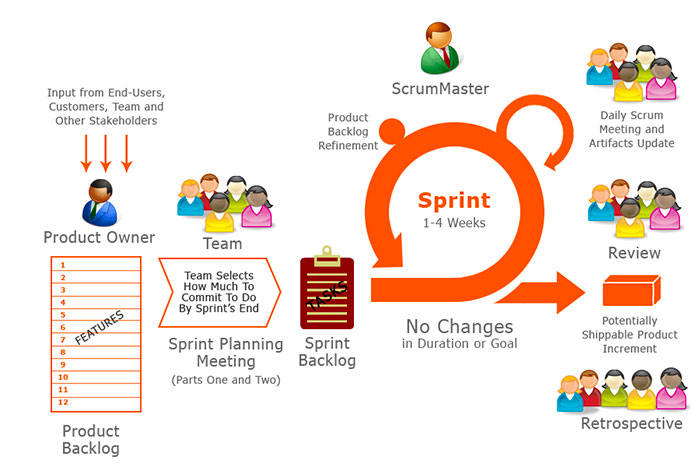
\includegraphics[scale=0.35]{immagini/scrum}
	\caption{Schema Scrum}
	\label{img:scrum}
\end{figure}
%**************************************************************
\section{Il progetto proposto}
Il progetto nasce dalla necessità di migliorare ed evolvere il sistema di \emph{\gls{IAM}}\glsfirstoccur sviluppato da parte dell'azienda.\\
Nelle sezioni seguenti si andrà quindi a discutere dettagliatamente il problema che si è voluto affrontare, le soluzioni che si sono trovate, l'ambito di sviluppo del prodotto, le funzionalità richieste e la pianificazione del progetto aziendale.

\subsection{Il contesto}
I servizi di identità decentralizzati permettono alle persone di registrarsi a specifici servizi come utenti in modo autonomo, utilizzando gli \emph{\gls{identityWallet}}\glsfirstoccur. 
Da questi gli utenti possono scegliere quali attributi del loro profilo immagazzinare e condividere con il \textit{service provider} verso il quale si vogliono autenticare.
Nella forma più semplice, l'identità è formata da due chiavi crittografiche, una pubblica ed una privata.
La chiave privata è mantenuta protetta all'interno dell'\gls{identityWallet}, mentre quella pubblica è crittografata tramite \textit{hash} e mantenuta immutabile all'interno dell'\gls{ITF}. 
La chiave privata viene utilizzata per crittografare le informazioni e gli attributi degli utenti, mentre quella pubblica viene utilizzata per decriptare le informazioni appena criptate. Questo meccanismo nasce allo scopo di assicurare che le informazioni criptate che arrivano al \textit{service provider} appartengano all'utente che effettivamente ha richiesto l'accesso al servizio. La sicurezza viene garantita proprio dal meccanismo delle chiavi in quanto solo l'utente stesso può conoscere la propria chiave privata e quindi criptare le proprie informazioni.\\
Le operazioni che avvengono, sia da parte dell'utente che del \textit{service provider}, per poter permettere l'accesso ad un servizio sono le seguenti:
\begin{enumerate}
	\item l'utente invia la richiesta d'accesso al \textit{service provider} inviando le proprie informazioni criptate con la sua chiave privata;
	\item il \textit{service provider} riceve le informazioni dell'utente e un suo identificativo;
	\item il \textit{service provider} interroga l'\gls{ITF} per recuperare la chiave pubblica associata a quell'utente;
	\item il \textit{service provider} decripta le informazioni dell'utente utilizzando la chiave pubblica recuperata.
\end{enumerate}
A questo punto il \textit{service provider} è sicuro che le informazioni che ha ricevuto sono di proprietà dell'utente e può permettere o meno l'accesso al servizio richiesto.\\
Questi passaggi sono la base di tre modelli di autenticazione:
\begin{itemize}
	\item Modello Centralizzato;
	\item Modello Decentralizzato;
	\item Modello basato sugli Identity Custodians.
\end{itemize}

\subsubsection{Modello Centralizzato}

In un modello centralizzato, le organizzazioni stabiliscono una relazione di fiducia \textit{punti a punto} con ogni utente che interagisce con il sistema (vedi Figura \ref{img:centralizzato}).
Le organizzazioni devono, quindi, mantenere la fiducia verso i loro utenti andando a gestire le varie identità digitali. Questo fa sì che le organizzazioni investano sulla protezione delle identità e delle informazioni sensibili. Questo si ripercuote, inevitabilmente, su un aumento dei costi operativi.\\
Dal lato utente questi non hanno alcun controllo sulla gestione delle proprie identità e attributi.\\
Ogni organizzazione deve verificare l'identità di ogni utente prima di permettere la registrazione e l'accesso ai suoi servizi. Questo può ripetersi molte volte per singolo utente a seconda dell'organizzazione cui l'utente richiede un servizio e a seconda del tipo di servizio che è richiesto. 
Questo modello ha fatto sì che nascesse una proliferazione di identità digitali diverse associate agli stessi utenti \cite{ITF_gartner}.
\begin{figure}[!h]
	\centering
	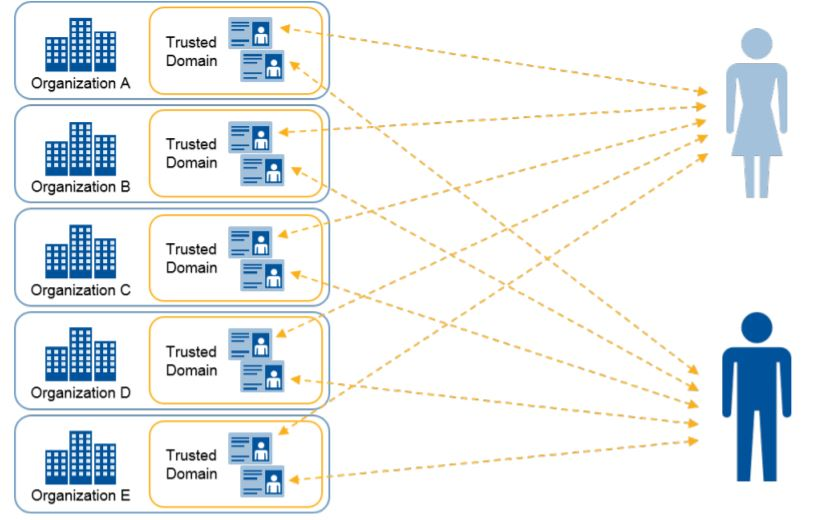
\includegraphics[scale=0.5]{immagini/ITF_Centralizzato}
	\caption{Modello Centralizzato}
	\label{img:centralizzato}
\end{figure}
\subsubsection{Modello Decentralizzato}

In un modello decentralizzato abbiamo un'entità terza che attesta e certifica la validità di un'identità auto-generata (vedi Figura \ref{img:decentralizzato}).
Questo tipo di modello non elimina il processo di identity proofing ma lo trasforma in un processo generalizzato che può essere utilizzato tra organizzazioni diverse.
Una volta che un'identità decentralizzata è stata legalmente provata, può essere utilizzata da service providers multipli per garantire l'accesso ai loro servizi.
Per far funzionare questo modello abbiamo bisogno di una "struttura" che immagazzini immutabilmente le informazioni e i certificati crittografati.  Per fare questo, la \textit{Blockchain} è la tecnologia adatta.
I sistemi decentralizzati alleviano le organizzazioni dell'incarico di mantenere informazioni sensibili riguardo l'identità con la conseguenza di abbassare i costi di mantenimento e di gestione dei rischi.
Dal lato utente invece abbiamo un controllo maggiore sulla privacy in quanto i sistemi decentralizzati permettono una miglior gestione delle identità personali e dei dati.
Tuttavia, la gestione completa delle informazioni personali, da parte dei singoli utenti, può risultare difficoltosa. È per questo che si è pensato di passare da un modello totalmente decentralizzato ad un modello ibrido dove le informazioni personali sono custodite dagli \textit{Identity Custiodians} \cite{ITF_gartner}.
\begin{figure}[!h]
	\centering
	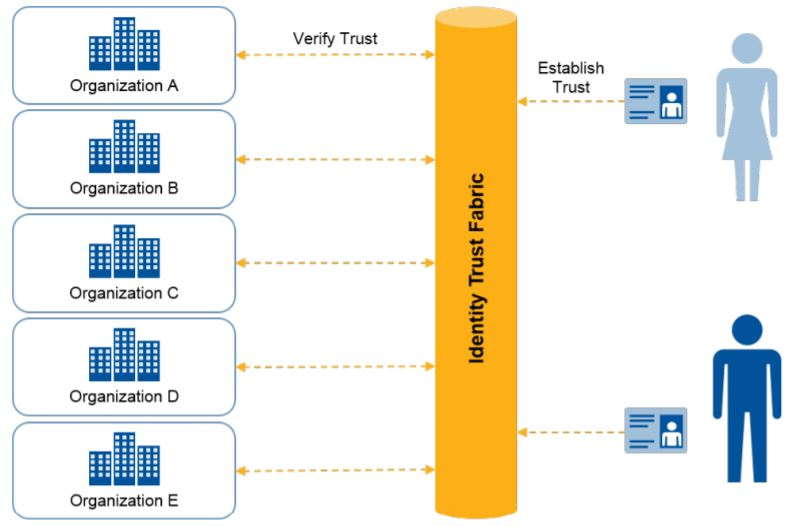
\includegraphics[scale=0.50]{immagini/ITF_Decentralizzato}
	\caption{Modello Decentralizzato}
	\label{img:decentralizzato}
\end{figure}
\subsubsection{Modello basato sugli Identity Custodians}
Gli \textit{Identity Custodians} nascono con l'obiettivo di semplificare la gestione e accrescere la disponibilità e protezione delle identità decentralizzate mantenendo, al loro interno, tutti gli attributi di identità necessari (vedi Figura \ref{img:identityCustodians}).
Sorgono spontanee alcune preoccupazioni in quanto, un \textit{Identity Custodian}, rimane suscettibile ad attacchi esterni in quanto mantiene informazioni sensibili e di valore nonostante siano criptate. Questo è il motivo alla base della creazione di consorzi che adempiono al compito di \textit{Identity Custodians} sfruttando la \textit{BlockChian} come tecnologia di decentralizzazione delle informazioni.\\
Utilizzando gli \textit{Identity Custodians} all'interno di un modello a consorzi si aumenta la privacy e la sicurezza delle informazioni. I dati utente ed i riferimenti ai loro hash nell'\gls{ITF} sono criptati e immagazzinati all'interno dell'ambiente decentralizzato. Questo permette all'\gls{identityWallet} di condividere solamente il riferimento alla locazione nell' \textit{Identity Custodian} facendo sì che i \textit{service provider} possano recuperare le informazioni e verificare l'identità utente prima dell'accesso\cite{ITF_gartner}.
\begin{figure}[h]
	\centering
	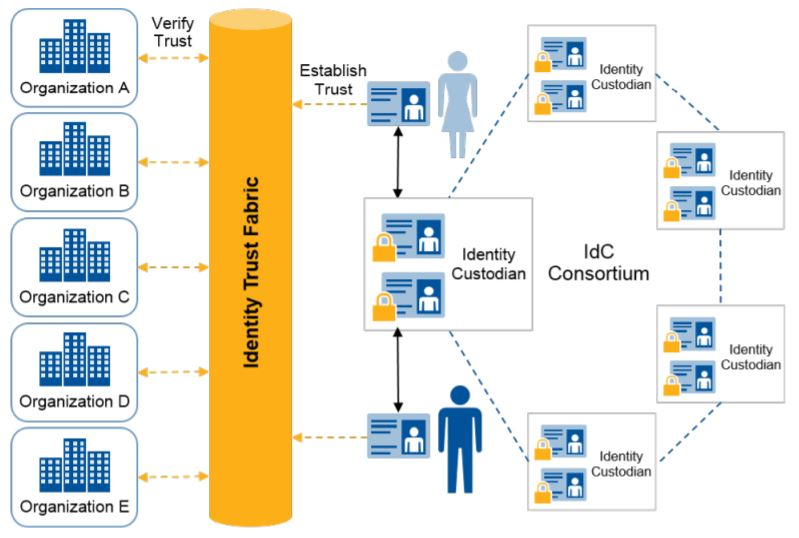
\includegraphics[scale=0.50]{immagini/ITF_IdentityCustodians}
	\caption{Modello basato sugli Identity Custodians}
	\label{img:identityCustodians}
\end{figure}

\subsection{Il progetto da realizzare}
Nell'ottica di estendere le funzionalità di \emph{\gls{monokee}}\glsfirstoccur, software di \textit{Identity and Access Management} in sviluppo presso Athesys, è stato previsto lo sviluppo di un layer di sicurezza, denominato \gls{ITF}, per integrare una tecnologia \textit{Blockchain} nei processi di accesso ai servizi e condivisione degli attributi di profilo.
\begin{figure}[!h]
	\centering
	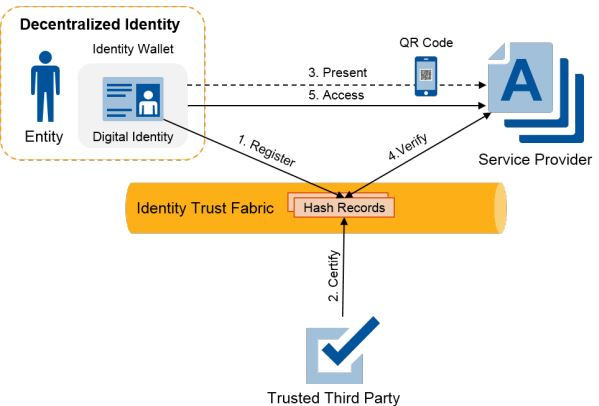
\includegraphics[scale=0.5]{immagini/ITF_Modello_Funzionale}
	\caption{Esempio di modello decentralizzato che sfrutta ITF}
	\label{fig:moduloITF}
\end{figure}
\\
La Figura \ref{fig:moduloITF} rappresenta un tipico scenario di accesso ai servizi di un \textit{service provider} da parte di un utente che possiede un proprio \gls{identityWallet}.
Il modulo realizzato rappresenta il layer di sicurezza che si interpone tra l'utente e i servizi offerti dal \textit{service provider}.
Le funzionalità principali realizzate durante lo stage, come si può vedere dalla figura, son essenzialmente cinque:
\begin{enumerate}
	\item \textbf{Registrazione}: come prima cosa l'utente genera la coppia di chiavi (privata e pubblica) nell'\gls{identityWallet}. La chiave pubblica viene crittografata tramite una funzione \textit{hash one-way} (ovvero calcolare l'hash è computazionalmente semplice, ma, partendo dall'hash, ricalcolare il valore originale è computazionalmente impossibile) e immagazzinata all'interno dell'\gls{ITF}. Al record, contenente l'identità, possono essere aggiunti ulteriori dati personali per rafforzare ancora di più il processo di \emph{\gls{identityProofing}}\glsfirstoccur e \emph{\gls{identityBinding}}\glsfirstoccur delle informazioni con l'identità digitale;
	 
	\item \textbf{Certificazione}: come parte del processo di \gls{identityProofing}, una parte terza fidata ha il compito di validare l'identità dell'utente. Questa validazione può avvenire o durante il processo di \gls{identityBinding} delle informazioni con l'identità digitale o durante la fase di registrazione/accesso di un utente ad un particolare servizio. Dopo aver validato con successo le informazioni di identità, questa parte terza certifica l'identità o gli attributi dell'utente, "firmandole" con la propria chiave privata. A questo punto il record certificato viene inserito nel \gls{ITF}.
	Il processo di registrazione/autenticazione può esser semplificato se esistono già dei record, interni all'\gls{ITF}, che contengono informazioni e attributi utili. 
	Su richiesta dell'utente, le organizzazioni possono ricertificare dei record per aumentare il livello di sicurezza delle informazioni contenute senza che l'utente debba registrarsi nuovamente generando un nuovo record con le stesse informazioni. Questo viene detto \textit{Web of Trust};
	 
	\item \textbf{Presentazione}: la chiave pubblica ed il riferimento alla locazione del \textit{hash} nel \gls{ITF} vengono forniti al \textit{service provider} affinché vengano verificati prima di permettere l'accesso al servizio;
	
	\item \textbf{Verifica}: una volta che il \textit{service provider} possiede la chiave pubblica, e la locazione dell'\textit{hash} nell'\gls{ITF} passa alla fase di verifica.
	In questa fase, utilizzando queste informazioni verifica l'identità o gli attributi utente andando a generare l'\textit{hash} dei dati e, successivamente, confrontandolo con il loro corrispettivo interno all'\gls{ITF};
	 
	\item \textbf{Accesso}: dopo aver verificato con successo l'identità di un utente viene concesso, a quest'ultimo, di accedere ai servizi o alle applicazioni richieste.
\end{enumerate}
\subsection{Obiettivi di stage}
Nella seguente tabella sono riportati gli obiettivi fissati per lo stage con rispettivo identificativo, importanza e breve descrizione.\\\\
L'identificativo (abbreviato in ID) userà la notazione:\\
\centerline{[\textit{Importanza}][\textit{numero identificativo}]}.\\
L'importanza sarà rappresentata da una delle seguenti lettere maiuscole:\\
\centerline{\textbf{O},\textbf{D},\textbf{F}}\\
che identificano, rispettivamente, un obiettivo obbligatorio, desiderabile o facoltativo.\\
Il numero identificativo è un numero incrementale che segnala in modo univoco l’obiettivo.\\
L'importanza di un obiettivo viene assegnata come segue:
\begin{itemize}
	\item \textbf{Obbligatorio} - rappresenta un requisito che dovrà esser soddisfatto al fine di garantire le funzionalità base del sistema;
	\item \textbf{Desiderabile} - rappresenta un requisito il cui non soddisfacimento non pregiudica le funzionalità base ma, la sua realizzazione, da un valore aggiunto importante al fine di realizzare un sistema più completo;
	\item \textbf{Facoltativo} - rappresenta un requisito che, se soddisfatto, renderebbe il sistema ancora più completo a discapito di un uso di risorse.
\end{itemize}
La Tabella \ref{tab:obiettiviDiStage} specifica meglio gli obiettivi di stage concordati nel piano di lavoro.
\begin{longtable}{|r l|p{3cm}|p{10cm}|}
	\hline
	\multicolumn{2}{|c|}{\textbf{ID}} & \textbf{IMPORTANZA} & \textbf{DESCRIZIONE}\tabularnewline
	\hline
	& O1 & Obbligatorio & Studio del dominio applicativo \\\hline
	& O2 & Obbligatorio & Studio delle possibili tecnologie \textit{Blockchain} da adottare \\\hline
	& O3 & Obbligatorio & Analisi comparativa delle tecnologie \textit{Blockchain} individuate \\\hline
	& O4 & Obbligatorio & Definizione dei vari casi d'uso per le funzionalità richieste \\\hline
	& O4.1 & Obbligatorio & Definizione dei casi d'uso per la funzionalità di registrazione \\\hline
	& O4.2 & Obbligatorio & Definizione dei casi d'uso per a funzionalità di certificazione \\\hline
	& O4.3 & Obbligatorio & Definizione dei casi d'uso per la funzionalità di verifica \\\hline
	& O5 & Obbligatorio & Stesura del documento di analisi dei requisiti\\\hline
	& O6 & Obbligatorio & Stesura del documento contenete le specifiche architetturali del sistema \\\hline
	& O7 & Obbligatorio & Realizzazione del modulo \gls{ITF}\\\hline
	& O7.1 & Obbligatorio & Realizzazione della struttura e della gerarchia di classi necessaria alla realizzazione del modulo \\\hline
	& O7.2 & Obbligatorio & Implementazione dei metodi necessari per il corretto funzionamento del modulo\\\hline
	& D1 & Desiderabile & Produzione della documentazione relativa alle analisi svolte \\\hline
	& D2 & Desiderabile & Definizione dei casi d'uso per la funzionalità di presentazione dei dati \\\hline
	& D3 & Desiderabile & Definizione dei casi d'uso per la funzionalità di accesso al servizio \\\hline
	& D4 & Desiderabile & Stesura del documento di progettazione\\\hline
	& D5 & Desiderabile & Realizzazione dei test necessari alla verifica del corretto funzionamento del sistema\\\hline
	& D5.1 & Desiderabile & Implementazione dei test di unità per i singoli metodi\\\hline
	& D5.2 & Desiderabile & Implementazione dei test di integrazione per testare le classi \\\hline
	& D5.3 & Desiderabile & Implementazione dei test di integrazione per testare l'interazione tra tutte le classi che compongono il sistema \\\hline
	& F1 & Facoltativo & Stesura del documento relativo ai test di unità ed integrazione \\\hline	
	& F2 & Facoltativo & Stesura del documento relativo alla validazione del modulo (anomalie e bug) \\\hline
	\caption{Tabella degli obiettivi di stage}
	\label{tab:obiettiviDiStage}
\end{longtable}
\subsection{Pianificazione del lavoro}
\label{sec:pianificazione_del_lavoro}
In accordo con l'azienda, tutto il periodo di stage che va dal 4 giugno 2018 al 30 luglio 2018 è stato suddiviso in fasi.\\
Vengono qui riportate in dettaglio le attività previste per ogni periodo, specificando il numero di ore preventivate e il periodo in cui ne è stato pianificato lo svolgimento.\\\\
\subsubsection{Fase 1: dal 4 giugno 2018 all'8 giugno 2018 per un totale di 40 ore}
In questa prima fase si era prevista l'individuazione della tecnologia \textit{Blockchain} da adottare per l'implementazione del modulo \gls{ITF}. La scelta della tecnologia prevedeva l'analisi ed il confronto delle varie tecnologie candidate in rapporto al dominio applicativo ovvero la gestione delle identità e degli accessi ai servizi.\\
In questa prima fase era prevista la stesura del documento di studio di Fattibilità.\\\\

\subsubsection{Fase 2: dall'11 giugno 2018 al 15 giugno 2018 per un totale di 40 ore}
In questa fase, lo scopo principale era studiare approfonditamente il sistema che si voleva realizzare e definire tutti i casi d'uso necessari per modellare, concettualmente, l'interno sistema.\\
Il mio stage prevedeva l'individuazione dei casi d'uso relativi alle funzionalità di:
\begin{itemize}
	\item Registrazione;
	\item Certificazione;
	\item Verifica.
\end{itemize}
Questa fase prevedeva la stesura del documento di Analisi dei Requisiti.\\\\

\subsubsection{Fase 3: dal 18 giugno 2018 al 22 giugno 2018 per un totale di 40 ore}
In questa terza fase è prevista la stesura dell'architettura generale, comprensiva di \emph{\gls{designPatterns}}\glsfirstoccur, per l'implementazione delle funzionalità rilevate dai casi d'uso della fase precedente.\\
Si è prevista anche la stesura del documenti di Progettazione Architetturale.\\\\

\subsubsection{Fase 4: dal 25 giugno 2018 al 4 luglio 2018 per un totale di 60 ore}
La quarta fase del periodo di stage prevede la definizione dei metodi necessari per l'implementazione del sistema in pseudo-codice. Anche in questa fase è prevista la stesura di un documento, desiderabile, di Progettazione di Dettaglio.\\\\

\subsubsection{Fase 5: dal 5 luglio 2018 al 25 luglio 2018 per un totale di 120 ore}
Fase centrale di tutto lo stage in cui è prevista la codifica del modulo \gls{ITF} comprensiva di classi e metodi.\\
Sempre durante questa fase era prevista anche la codifica dei test di unità e di integrazione per i singoli metodi e per le classi.\\
A corredo di tutto questo era prevista la stesura del documento relativo al testing delle funzionalità.\\\\

\subsubsection{Fase 6: dal 26 luglio 2018 al 30 luglio 2018 per un totale di 20 ore}
In quest'ultima fase è prevista la validazione dell'intero sistema realizzato e predisposto il software per il collaudo finale fatto in coordinamento con l'altro studente stagista che ha realizzato le componenti mancanti per l'implementazione del modulo \gls{ITF} finale.\\\\

Al termine di questo periodo di stage il prodotto si trova in una fase di \emph{\gls{poc}}\glsfirstoccur funzionante e predisposta per:
\begin{itemize}
	\item poter implementare nuove future funzionalità;
	\item migliorare le funzionalità che già possiede senza dover apportare grossi cambiamenti all'infrastruttura;
	\item permettere l'integrazione come parte del prodotto cardine dell'azienda: \gls{monokee}.
\end{itemize}

\subsubsection{Riepilogo delle attività previste}
In Tabella \ref{tab:riepilogoOre} si ha un riepilogo delle attività di stage previste.
\begin{longtable}{|r l|p{1cm}|p{3cm}|}
	\hline
	\multicolumn{2}{|c|}{\textbf{ATTIVITÀ}} & \textbf{ORE} & \textbf{PERIODO}\tabularnewline
	\hline
	& Fase 1 & \centerline{40} & 08/06 - 22/06 \\\hline	
	& Fase 2 & \centerline{40} & 11/06 - 15/06\\\hline
	& Fase 3 & \centerline{40} & 18/06 - 22/06\\\hline
	& Fase 4 & \centerline{60} & 25/06 - 04/07 \\\hline
	& Fase 5 & \centerline{120} & 05/07 - 25/07 \\\hline
	& Fase 6 & \centerline{20} & 26/07 - 30/07 \\\hline	
	\caption{Riepilogo delle attività di stage previste}
	\label{tab:riepilogoOre}
\end{longtable}

\section{Analisi preventiva dei rischi}

Durante la fase di analisi iniziale sono stati individuati alcuni possibili rischi.
Si è quindi proceduto a elaborare delle possibili soluzioni per far fronte a tali rischi.\\

\begin{risk}{Tecnologia Blockchain}
	\riskdescription{Avendo a che fare con una tecnologia mai utilizzata prima ed in costante sviluppo, vi è la possibilità di subire rallentamenti per approfondire nuove tematiche e risolvere problemi legati allo sviluppo}
	\risksolution{L'unica soluzione possibile è lo studio individuale e l'approfondimento della tematica}
	\label{risk:new-technology}
\end{risk}

\begin{risk}{Nuovo linguaggio: Solidity}
	\riskdescription{Avendo a che fare con una tecnologia diversa dal solito, anche il linguaggio di programmazione che ne permette l'utilizzo è diverso. Il rischio è che le conoscenze acquisite in termini di \textit{Design Patterns} o scelte architetturali potrebbero non essere più valide nel nuovo contesto}
	\risksolution{Bisogna adattare le conoscenze pregresse alla nuova tecnologia in modo da risolvere le problematiche riscontrate}
	\label{risk:different-way-of-thinking}
\end{risk}

\begin{risk}{Nuovi strumenti per la gestione della tecnologia}
	\riskdescription{Anche gli strumenti a supporto della tecnologia \textit{Blockchain} possono dare problemi in quanto, molti di questi, sono ancora in versioni \textit{beta} o rilasciati in versioni stabili da poco. In più, essendo una tecnologia relativamente nuova, si può incorrere nel rischio di trovare anomalie e bug non ancora risolti}
	\risksolution{La soluzione è lo studio approfondito della tematica e del dominio applicativo insieme ad un approfondimento di cosa questi strumenti permettono di fare e di come raggiungono il loro scopo}
	\label{risk:new-tools}
\end{risk}
%**************************************************************
             % Introduzione
% !TEX encoding = UTF-8
% !TEX TS-program = pdflatex
% !TEX root = ../tesi.tex

%**************************************************************
\chapter{Tecnologie e strumenti}
\label{cap:tecnologie_e_strumenti}
%**************************************************************
In questo capitolo verranno illustrate le tecnologie e gli strumenti che sono stati utilizzati per realizzare il progetto di stage.\\
Il capitolo si apre con una descrizione di che cos'è una \textit{Blockchain} e del perchè è stata scelta come tecnologia chiave per la realizzazione del progetto e, di seguito, verranno descritti tutti gli strumenti utilizzati.\\\\
Questa sezione è frutto di studi di vari documenti e \textit{whitepaper} forniti dall'azienda\cite{spidchain_whitepaper}\cite{SSID}\cite{jolocom_whitepaper}\cite{ITF_gartner}\cite{hashgraph_whitepaper}
%**************************************************************
\section{Cos'è una Blockchain}
Una \textit{Blockchain} è un \emph{\gls{dlt}}\glsfirstoccur che si basa fortemente sul \textit{consenso} e su un sistema di \textit{smart contracts}.
È quindi una piattaforma costruita su una rete di nodi (detti blocchi) distribuiti dove gli elementi chiave che la contraddistinguono sono:
\begin{itemize}
	\item \textbf{Smart Contracts} - programmi che vengono eseguiti solamente quando si verificano determinate condizioni;
	\item \textbf{Consenso} - sistema che assicura che la maggioranza (50\% + 1) dei nodi della rete identifichi e sia in accordo, con tutti gli altri nodi della rete, che un determinato stato del sistema sia quello esatto.
\end{itemize}
Questi blocchi sono formati da quattro sezioni:
\begin{itemize}
	\item \textbf{Block size} che rappresenta la grandezza in bytes del blocco;
	\item \textbf{Block Header} è un campo particolare che è a sua volta formato da:
	\begin{itemize}
		\item \textbf{Version} numero di versione del software utilizzato;
		\item \textbf{Previous Block Hash} contiene l'hash dell'header del blocco precedente.;
		\item \textbf{Markle root} hash della radice del \textit{Markle tree} (spiegato di seguito);
		\item \textbf{Timestamp} tempo di creazione del blocco;
		\item \textbf{Difficulty target} numero che indica il livello di difficolta per l'aggiunta del blocco alla \textit{Blockchain};
		\item \textbf{numero casuale o pseudo-casuale dato come risultato dell'elaborazione della\emph{\gls{pow}}\glsfirstoccur}.
	\end{itemize}
	\item \textbf{Transaction counter} contiene il numero di transazioni che compongono il blocco;
	\item \textbf{Transaction} lista di tutte le transazioni che verranno processate nel blocco.
\end{itemize}
\subsection{Caratteristiche chiave}
             % Processi
% !TEX encoding = UTF-8
% !TEX TS-program = pdflatex
% !TEX root = ../tesi.tex

%**************************************************************
\chapter{Analisi dei requisiti}
\label{cap:analisi_dei_requisiti}
%**************************************************************
In questo capitolo verranno esposti i casi d'uso e i requisiti del modulo \gls{ITF} che erano oggetto del lavoro di stage.\\
Si procede con la descrizione dello stato del sistema, gli attori che vi partecipano, le pre-condizioni, le post-condizioni e gli scenari.\\
I casi d'uso principali sono associati ad un diagramma \gls{uml} 2.0 che riporta lo stesso codice identificativo e titolo del caso d'uso al quale si riferisce.

%**************************************************************
\section{Dominio}
\subsection{Caratteristiche degli attori}
L'interazione con il modulo \gls{ITF} coinvolge essenzialmente tre tipologie diverse di attori:
\begin{itemize}
	\item L'identity wallet;
	\item Un ente certificatore;
	\item Un service provider.
\end{itemize}

\subsubsection{Identity Wallet}
Questa componente del sistema ha il compito di generare, mantenere e presentare l'identità digitale dell'utente. A sua volta, l'\textit{Identity Wallet} interagisce con il sistema \gls{ITF} nel momento in cui un utente esegue una richiesta di accesso verso un \textit{service provider} il quale richiede l'autenticazione e la conferma delle credenziali insieme alla verifica di attributi specifici necessari per erogare i suoi servizi.\\
Il sistema \gls{monokee}, una volta che l'utente richiede l'accesso ad un \textit{service provider}, reindirizza la richiesta di accesso all'\gls{ITF}.
\subsubsection{Ente Certificatore (Trusted Third Party)}
La seconda tipologia di attori che interagiscono con il sistema da realizzare sono i \textit{Trusted Third Party}.\\
Questi, chiamati enti certificatori, hanno il compito di certificare le informazioni che sono presenti all'interno dell'\gls{ITF} in modo che, ogni qual volta che vengono richieste informazioni per poter accedere ad un \textit{service provider}, le informazioni che il sistema fornisce per l'autenticazione e/o l'erogazione di servizi, siano verificate da un ente esterno che garantisce la loro veridicità.
\subsubsection{Service Provider}
La terza e ultima tipologia di attori che partecipano al sistema sono i \textit{service provider}.
Questi interagiscono con l'\gls{ITF} durante la fase di verifica delle informazioni. Questi devono autenticare gli utenti tramite le loro credenziali e autorizzare l'erogazione di servizi dopo la verifica degli attributi
%**************************************************************
\subsection{Overview del sistema}
Una rappresentazione delle funzionalità che deve implementare il modulo \gls{ITF} può essere ripresa in figura \ref{fig:moduloITF}.\\\\
Il prodotto finale prevede l'interazione delle tre tipologie di attori allo scopo di garantire:
\begin{itemize}
	\item L'accesso sicuro al \textit{service provider} desiderato;
	\item L'erogazione dei servizi offerti dal \textit{service provider} in modo controllato.
\end{itemize}
Questo viene garantito dall'\gls{ITF} e dalla tecnologia \textit{Blockchain} che ne è alla base.\\
Di seguito viene descritto il flusso di chiamate che intercorrono affinchè un utente possa accedere ad uno o più servizi di sua scelta.\\\\
Quando un utente richiede dei servizi, da parte di un \textit{service provider}, il sistema viene interrogato e inizia lo scambio di informazioni che coinvolge l'\textit{identity wallet}, gli enti certifictori ed il \textit{service provider}.\\
Ogni qual volta un utente richiede l'accesso a dei servizi di un determinato \textit{service provider}, \gls{monokee} reindirizza la richiesta d'accesso all'\textit{identity wallet} che, a sua volta, invia la richiesta di accesso all'\gls{ITF} passandogli un identificativo dell'utente che ha fatto la richiesta di accesso insieme alle informazioni che il \textit{service provider} necessita per poter permettere l'erogazione dei suoi servizi.\\
Nell'\gls{ITF} viene eseguita una ricerca nella rete \textit{Blockchain} sottostante in modo da verificare se le informazioni richieste dal \textit{service provider} siano efffettivamente associate all'utente. Se il riscontro è positivo, il \textit{service provider} permette l'accesso all'utente altrimenti gli viene negato.\\\\
La seconda tipologia di attori che partecipano al sistema, gli enti certificatori, entrano in gioco durante la fase di registrazione di un nuovo utente o quando un amministratore di dominio associa degli attributi alle identità digitali dei suoi utenti.
Gli enti certificatori hanno il compito di verificare e certificare che, le asserzioni o gli attributi, di una particolare identità, siano conformi alle informazioni associate a quell'utente.\\
Questo ruolo è di fondamentale importanza all'interno del sistema che si sta sviluppando in quanto, essendo l'\gls{ITF} basata su una \textit{Blockchain}, tutte le informazioni che popolano la rete sono immutabili e, quindi, prima di essere definitivamente inserite in un blocco, devono essere verificate e approvate, dagli enti certificatori, tramite gli algoritmi di consenso.\\\\
La terza tipologia di attori, i \textit{service providers}, interagiscono con il sistema durante la verifica delle informazioni dell'identità dell'utente.\\
Questi, dopo che l'\textit{identity wallet} gli ha passato i record contenenti la chiave pubblica e il riferimento alla locazione del record cifrato nell'\gls{ITF}, iniziano il  controllo delle informazioni.\\
Il controllo viene fatto andando prima a calcolare l'\textit{hash crittografico} della chiave pubblica pervenuta dall'\textit{identity wallet} e poi andando a confrontare il risultato ottenuto con quello presente nell'\gls{ITF} recuperato grazie al riferimento alla sua locazione nella rete Blockchain.
In questa fase, il \textit{service provider} verifica i record contenente l'identità e qualsiasi altra credenziale per autenticare l'utente e verifica anche gli attributi necessari per autorizzare l'utente ad utilizzare i suoi servizi.
\section{Casi d'uso}
\subsection{Classificazione dei casi d'uso}
Ogni caso d'uso è classificato secondo la seguente convienzione:\\\\
\centerline{UC[codicePadre]\_[codiceFiglio]}\\\\
In cui i due codici rappresentano:
\begin{itemize}
	\item \textbf{codicePadre} - identifica univocamente il caso d'uso;
	\item \textbf{codiceFiglio} - identifica univocamente i sotto casi d'uso apparteneti ad un determinato "codicePadre".
\end{itemize}

\subsection{Descrizione dei casi d'uso}
Ogni caso d'uso viene descritto dalla seguente struttura:
\begin{itemize}
	\item \textbf{Descrizione} - Breve descrizione del caso d'uso che si sta modellando;
	\item \textbf{Attori Principali} - Indica l'attore principale del caso d'uso. In tutto il contesto dell'applicazione, gli attori saranno classificati come:
	\begin{itemize}
		\item Identity Wallet;
		\item Trusted Third Party (ente certificatore);
		\item Service Provider.
	\end{itemize}
	\item \textbf{Attori Secondari} - Indica l'attore che aiuta l'attore principale a realizzare quanto descritto dal caso d'uso;
	\item \textbf{Pre-Condizioni} - Specifica la condizione del sistema prima del verificarsi degli eventi descritti dal caso d'uso;
	\item \textbf{Post-Condizioni} - Specifica le condizioni del sistema dopo il verificarsi degli eventi descritti dal caso d'uso;
	\item \textbf{Scenario Principale} - Rappresenta il flusso principale degli eventi ovvero il caso in cui tutto funzioni come deve;
	\item \textbf{Estensioni} - Rappresenta il flusso secondario degli eventi nel caso in cui si verifichino degli errori nel flusso principale.
\end{itemize}

\subsection{Caso d'uso UC1: Registrazione}
\begin{figure}[h]
	\centering
	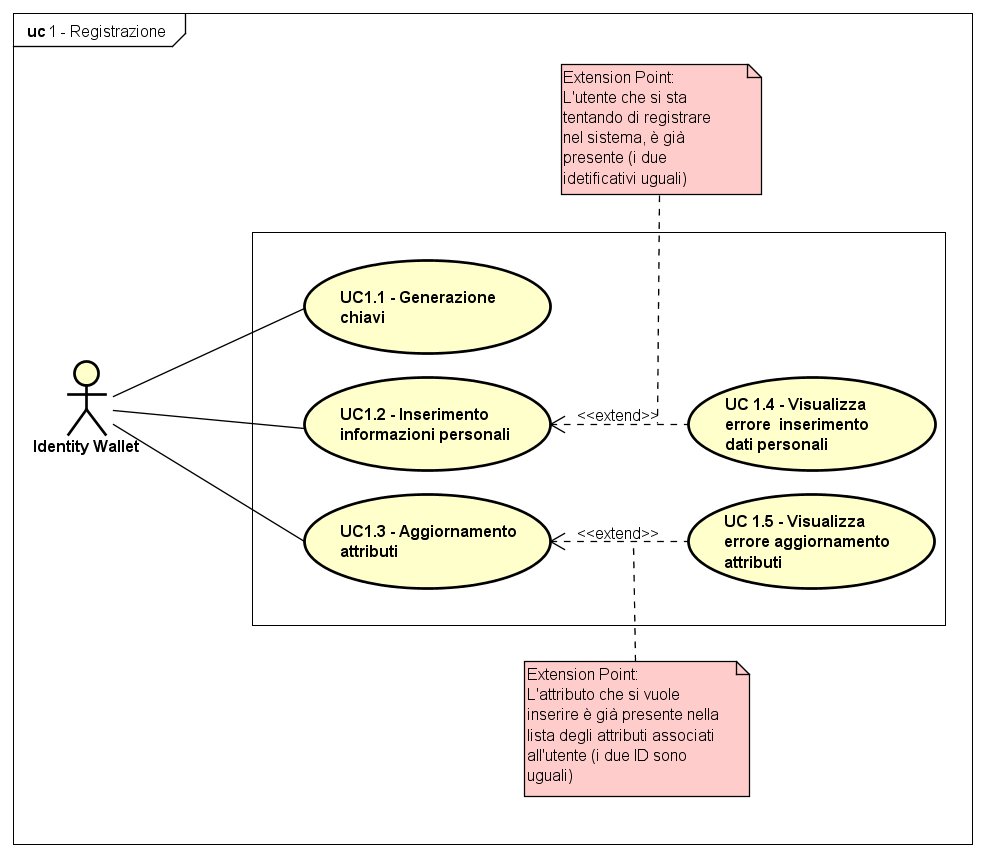
\includegraphics[scale=0.50]{immagini/usecase/UC1_Registrazione}
	\caption{Caso d'uso UC1: Registrazione}
\end{figure}
\begin{itemize}
	\item \textbf{Descrizione} - L'Identity Wallet genera la chiave pubblica, quella privata ed inserisce le informazioni personali dell'utente. In alternativa può aggiornare gli attributi esistenti aggiungendone di nuovi;
	\item \textbf{Attori Principali} - Identity Wallet;
	\item \textbf{Attori Secondari} -
	\item \textbf{Pre-Condizioni} - L'Identity Wallet non possiede un identità digitale per l'utente;
	\item \textbf{Post-Condizioni} - L'Identity Wallet ha creato un identità per l'utente ed è in attesa che questa venga certificata;
	\item \textbf{Scenario Principale} - 
	\begin{enumerate}
		\item Generazione delle chiavi (UC 1.1);
		\item Inserimento delle informazioni personali (UC 1.2);
		\item Aggiornamento degli attributi già presenti nell'\gls{ITF} (UC 1.3);
	\end{enumerate}
	\item \textbf{Estensioni} -
	\begin{enumerate}
		\item All'Identity Wallet viene segnalato un errore di registrazione del nuovo utente (UC 1.4);
		\item All'Identity Wallet viene segnalato un errore sull'aggiornamento degli attributi (UC 1.5).
	\end{enumerate}
\end{itemize}
\subsection{Caso d'uso UC1.1: Generazione Chiavi}
\begin{figure}[h]
	\centering
	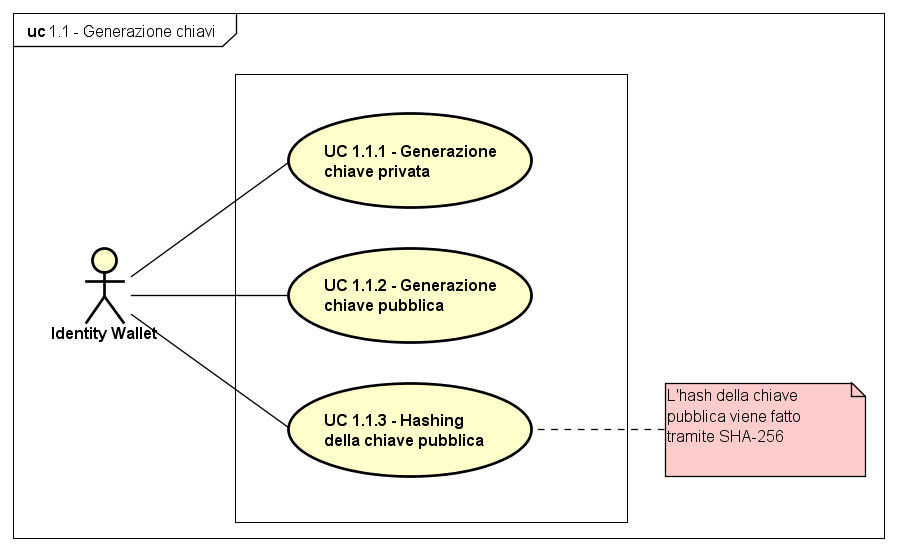
\includegraphics[scale=0.50]{immagini/usecase/UC11_GenerazioneChiavi}
	\caption{Caso d'uso UC1.1: Generazione chiavi}
\end{figure}
\begin{itemize}
	\item \textbf{Descrizione} - L'Identity Wallet genera la chiave privata e quella pubblica. Quest'ultima viene crittografata tramite \textit{hash} e rappresenta l'identità digitale dell'utente;
	\item \textbf{Attori Principali} - Identity Wallet;
	\item \textbf{Attori Secondari} -
	\item \textbf{Pre-Condizioni} - L'Identity Wallet non possiede una coppia di chiavi pubblica-privata;
	\item \textbf{Post-Condizioni} - L'Identity Wallet è in possesso di una coppia di chiavi (pubblica e privata) e del \textit{hash} di quella pubblica;
	\item \textbf{Scenario Principale} -
	\begin{enumerate}
		\item Generazione della chiave privata (UC 1.1.1);
		\item Generazione della chiave pubblica (UC 1.1.2);
		\item Generazione del \textit{hash} della chiave pubblica (UC 1.1.3).
	\end{enumerate}
	\item \textbf{Estensioni} -
\end{itemize}
\subsection{Caso d'uso UC1.2: Inserimento informazioni personali}
\begin{figure}[h]
	\centering
	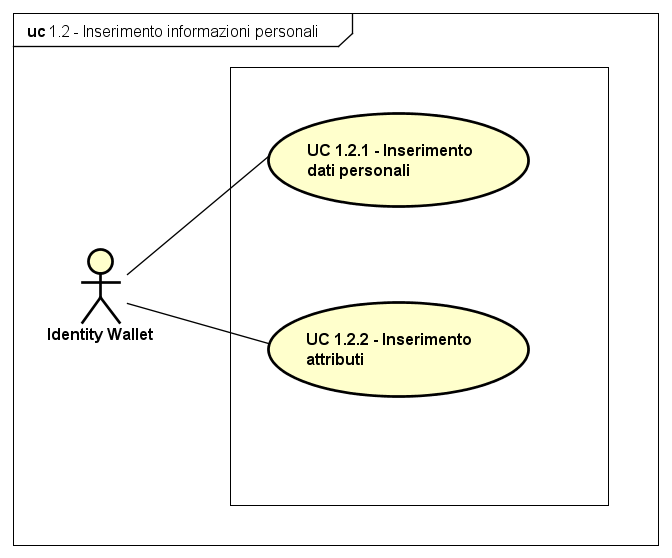
\includegraphics[scale=0.50]{immagini/usecase/UC12_InserimentoInformazioniPersonalii}
	\caption{Caso d'uso UC1.2: Inserimento informazioni personali}
\end{figure}
\begin{itemize}
	\item \textbf{Descrizione} - L'Identity Wallet crea l'identità digitale dell'utente come un insieme di dati personali e attributi a lui associati;
	\item \textbf{Attori Principali} - Identity Wallet;
	\item \textbf{Attori Secondari} -
	\item \textbf{Pre-Condizioni} - L'Identity Wallet non possiede le informazioni personali dell'utente ed i suoi attributi;
	\item \textbf{Post-Condizioni} - L'Identity Wallet possiede tutte le informazioni personali dell'utente ed i suoi attributi;
	\item \textbf{Scenario Principale} -
	\begin{enumerate}
		\item Inserimento dei dati personali utente (UC 1.2.1);
		\item Inserimento dei degli attributi utente (UC 1.2.2);
	\end{enumerate}
	\item \textbf{Estensioni} -
\end{itemize}
\subsection{Caso d'uso UC1.2.1: Inserimento dati personali utente}
\begin{figure}[h]
	\centering
	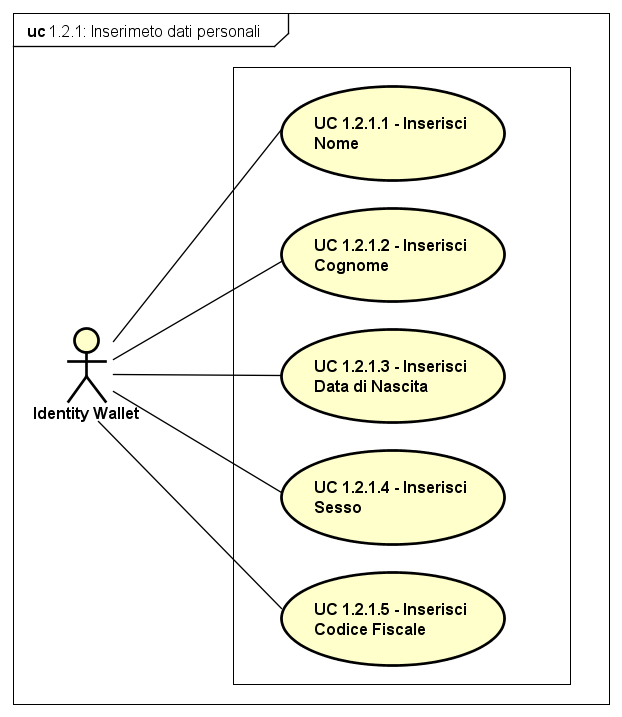
\includegraphics[scale=0.50]{immagini/usecase/UC121_InserimentoDatiPersonali}
	\caption{Caso d'uso UC1.2.1: Insierimento dati personali utente}
\end{figure}
\begin{itemize}
	\item \textbf{Descrizione} - L'Identity Wallet compila i campi dedicati alle informazioni personali dell'identità utente che vuole registrare all'ITF;
	\item \textbf{Attori Principali} - Identity Wallet;
	\item \textbf{Attori Secondari} -
	\item \textbf{Pre-Condizioni} - L'Identity Wallet non ha inserito le informazioni personali dell'identità utente che vuole registrare nell'\gls{ITF};
	\item \textbf{Post-Condizioni} - L'Identity Wallet ha inserito tutte le informazioni personali dell'identità utente che vuole registrare nell'\gls{ITF};
	\item \textbf{Scenario Principale} -
	\begin{enumerate}
		\item Inserimento del nome dell'utente (UC 1.2.1.1);
		\item Inserimento del cognome dell'utente (UC 1.2.1.2);
		\item Inserimento della data di nascita (UC 1.2.1.3);
		\item Inserimento del sesso dell'utente (UC 1.2.1.4);
		\item Inserimento del codice fiscale (UC 1.2.1.5).
	\end{enumerate}
	\item \textbf{Estensioni} -
\end{itemize}
\subsection{Caso d'uso UC1.2.2: Inserimento attributi}
\begin{figure}[h]
	\centering
	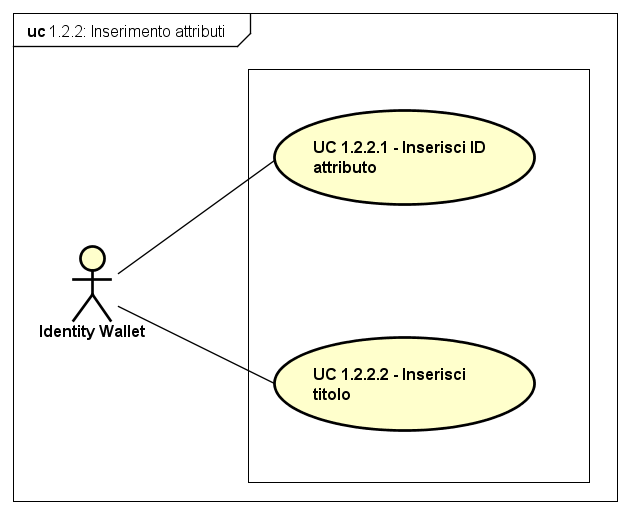
\includegraphics[scale=0.50]{immagini/usecase/UC122_InserimentoAttributi}
	\caption{Caso d'uso UC1.2.2: Insierimento attributi}
\end{figure}
\begin{itemize}
	\item \textbf{Descrizione} -L'Identity Wallet compila i campi dedicati agli attributi/certificazioni per creare l'identità digitale dell'utente;
	\item \textbf{Attori Principali} - Identity Wallet;
	\item \textbf{Attori Secondari} -
	\item \textbf{Pre-Condizioni} - L'Identity Wallet non possiede le informazioni inerenti agli attributi/certificazioni dell'utente che sta registrando nell'\gls{ITF};
	\item \textbf{Post-Condizioni} - L'Identity Wallet possiede tutte le informazioni inerenti agli attributi/certificazioni dell'utente che sta registrando nell'\gls{ITF};
	\item \textbf{Scenario Principale} -
	\begin{enumerate}
		\item Inserimento dell'ID che individua l'attributo (UC 1.2.2.1);
		\item Insierimento del titolo che descrive l'attributo (UC 1.2.2.2).
	\end{enumerate}
	\item \textbf{Estensioni} -
\end{itemize}
\subsection{Caso d'uso UC1.3: Aggiornamento attributi}
\begin{figure}[h]
	\centering
	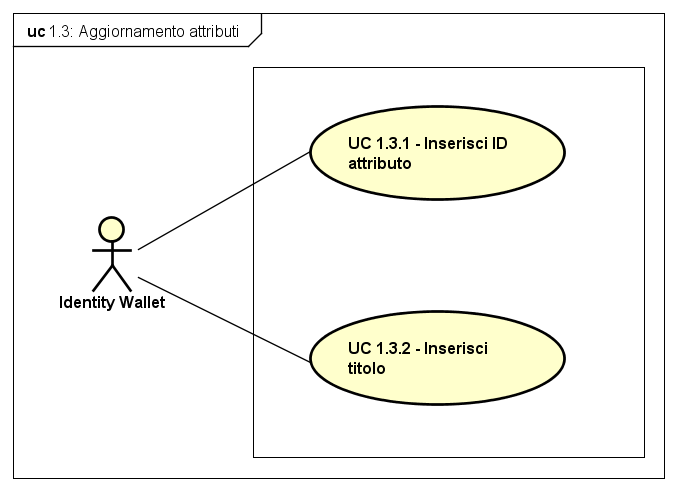
\includegraphics[scale=0.50]{immagini/usecase/UC13_AggiornamentoAttributi}
	\caption{Caso d'uso UC1.3: Aggiornamento attributi}
\end{figure}
\begin{itemize}
	\item \textbf{Descrizione} - L'Identity Wallet aggiorna gli attributi/certificazioni dell'utente, aggiungendone di nuove alla lista di quelle già presente nell'\gls{ITF};
	\item \textbf{Attori Principali} - Identity Wallet;
	\item \textbf{Attori Secondari} -
	\item \textbf{Pre-Condizioni} - L'Identity Wallet vuole aggiornare la lista di attributi/certificazioni associati all'utente;
	\item \textbf{Post-Condizioni} - L'Identity Wallet ha aggiornato la lista di attributi/certificazioni associati all'utente;
	\item \textbf{Scenario Principale} -
	\begin{enumerate}
		\item Inserimento dell'ID corrispondente all'attributo (UC 1.3.1);
		\item Inserimento del titolo descrittivo dell'attributo (UC 1.3.2).
	\end{enumerate}
	\item \textbf{Estensioni} -
\end{itemize}
\subsection{Caso d'uso UC1.4: Visualizza errore registrazione utente}
\begin{itemize}
	\item \textbf{Descrizione} - All'Identity Wallet viene segnalata, tramite un opportuno errore, l'impossibilità di creare e registrare una nuova identità digitale per l'utente. Questo avviene quando si tenta di registrare un'identità che è già presente nel sistema;
	\item \textbf{Attori Principali} - Identity Wallet;
	\item \textbf{Attori Secondari} -
	\item \textbf{Pre-Condizioni} - L'Identity Wallet vuole registrare una nuova identityà digitale per l'utente;
	\item \textbf{Post-Condizioni} - L'Identity Wallet non è riuscito a registrare la nuova identityà digitale nell'\gls{ITF};
	\item \textbf{Scenario Principale} -
	\begin{enumerate}
		\item All'Identity Wallet viene segnalata, tramite un errore, l'impossibilità di registrare il nuovo utente al sistema (UC 1.4);
	\end{enumerate}
	\item \textbf{Estensioni} -
\end{itemize}
\subsection{Caso d'uso UC1.5: Visualizza errore aggioranemento attributo}
\begin{itemize}
	\item \textbf{Descrizione} - All'Identity Wallet viene segnalata, tramite un opportuno errore, l'impossibilità di aggiornare la lista di attributi/certificazioni dell'utente. Questo avviene quando si tenta di aggiornare un attributo/certificazione che non è presente nell'\gls{ITF};
	\item \textbf{Attori Principali} - Identity Wallet;
	\item \textbf{Attori Secondari} -
	\item \textbf{Pre-Condizioni} - L'Identity Wallet vuole aggiornare la lista degli attributi e certificazioni associati all'utente;
	\item \textbf{Post-Condizioni} - La lista non è stata aggiornata;
	\item \textbf{Scenario Principale} -
	\begin{enumerate}
		\item All'Identity Wallet viene segnalata, tramite un errore, l'impossibilità di agiornare gli attributi (UC 1.5);
	\end{enumerate}
	\item \textbf{Estensioni} -
\end{itemize}
\subsection{Caso d'uso UC2: Certificazione}
\begin{figure}[h]
	\centering
	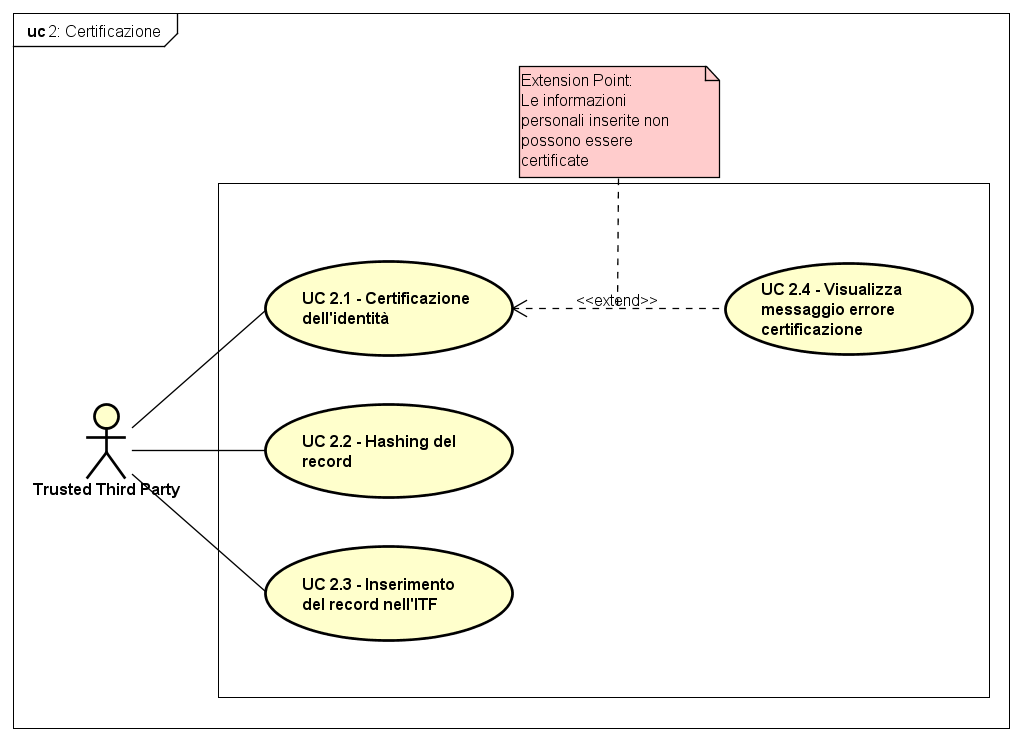
\includegraphics[scale=0.50]{immagini/usecase/UC2_Certificazione}
	\caption{Caso d'uso UC2: Certificazione}
\end{figure}
\begin{itemize}
	\item \textbf{Descrizione} - L'attore vuole certificare tutte le informazioni riguardanti l'identità digitale dell'utente e, una volta certificate, inserirle nell'\gls{ITF}.\\
	La certificazione avviene grazie alla firma, delle informazioni personali e degli attributi, tramite la chiave privata dell'attore. Una volta firmate, le informazioni vengono inserite in un record, fatto l'\textit{hash} del record e quindi inserito nell'\gls{ITF};	
	\item \textbf{Attori Principali} - Trusted Third Party;
	\item \textbf{Attori Secondari} -
	\item \textbf{Pre-Condizioni} - L'attore vuole certificare l'identità e gli attributi di un particolare utente;
	\item \textbf{Post-Condizioni} - La Trusted Third Party ha certificato correttamente l'identità e gli attributi dell'utente e ha inserito il record nell'\gls{ITF};
	\item \textbf{Scenario Principale} -
	\begin{enumerate}
		\item L'attore certifica le informazioni dell'utente (UC 2.1);
		\item L'attore esegue l'\textit{hash} del record contenente tutte le informazioni appena certificate (UC 2.2);
		\item L'attore, una volta fatto l'\textit{hash} del record, lo inserisce nell'\gls{ITF} (UC 2.3).
	\end{enumerate}
	\item \textbf{Estensioni} -
	\begin{enumerate}
		\item Visualizza messaggio d'errore nella certificazione delle informazioni personali (UC 2.4).
	\end{enumerate}
\end{itemize}
\subsection{Caso d'uso UC2.1: Certificazione dell'identità}
\begin{figure}[h]
	\centering
	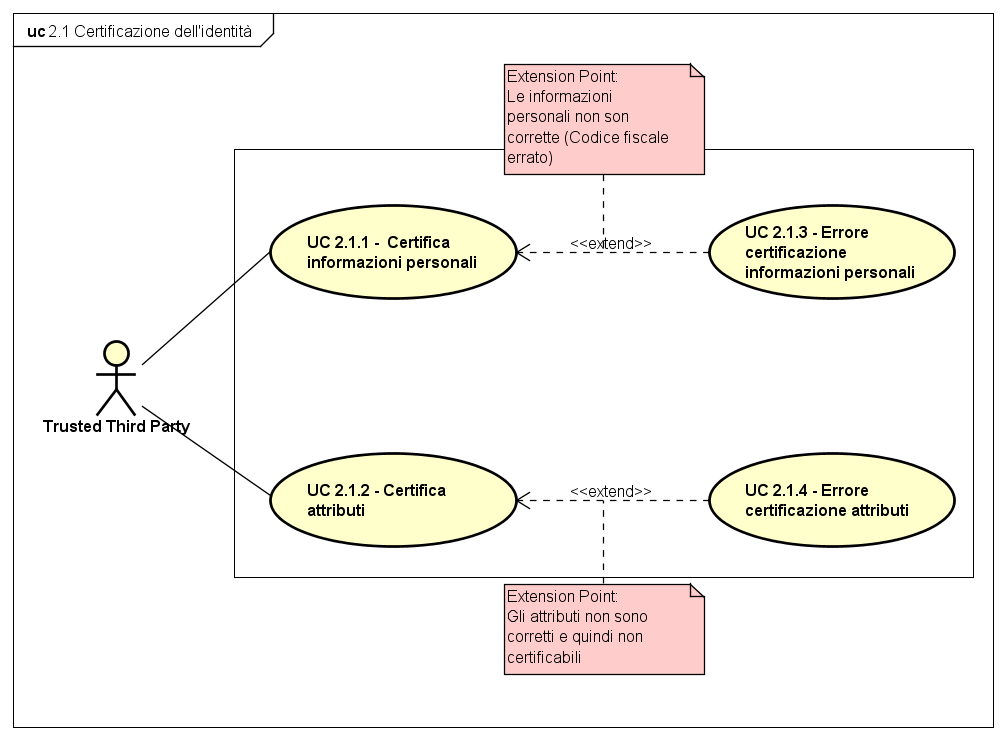
\includegraphics[scale=0.50]{immagini/usecase/UC21_CertificazioneIdentita}
	\caption{Caso d'uso UC2.1: Certificazione dell'identità}
\end{figure}
\begin{itemize}
	\item \textbf{Descrizione} - La Trusted Third Party, prima di inserire il record nell'ITF, deve certificare tutte le informazioni personali associate all'utente (dati e attributi/certificazioni).\\
	Questo viene fatto grazie alla firma, dei dati e degli attributi, tramite chiave privata della Trusted Third Party;
	\item \textbf{Attori Principali} - Trusted Third Party;
	\item \textbf{Attori Secondari} -
	\item \textbf{Pre-Condizioni} - L'attore vuole certificare tutte le informazioni personali dell'utente;
	\item \textbf{Post-Condizioni} - L'attore ha certificato tutte le informazioni personali dell'utente;
	\item \textbf{Scenario Principale} -
	\begin{enumerate}
		\item Certificazione delle informazioni personali tramite chiave privata (UC 2.1.1);
		\item Certificazione degli attributi/certificazioni tramite chiave privata (UC 2.1.2).
	\end{enumerate}
	\item \textbf{Estensioni} -
	\begin{enumerate}
		\item Visualizza errore nella certificazione delle informazioni personali (UC 2.1.3);
		\item Visualizza errore nella certificazione degli attributi (UC 2.1.4).
	\end{enumerate}
\end{itemize}
\subsection{Caso d'uso UC 2.4: Visualizza errore certificazione dell'identità}
\begin{itemize}
	\item \textbf{Descrizione} - Alla Trusted Third Party viene segnalata l'impossibilità di certificare uno o più informazioni personali dell'utente (dati personali, attributo o certificazioni).\\
	Questo avviene quando, la Trusted Third Party, non riesce a trovare corrispondenza tra gli attributi e i dati indicati con l'identità dell'utente;
	\item \textbf{Attori Principali} - Trusted Third Party;
	\item \textbf{Attori Secondari} - L'attore vuole certificare tutte le informazioni personali dell'utente (dati personali e attributi);
	\item \textbf{Pre-Condizioni} -
	\item \textbf{Post-Condizioni} - L'attore non è riuscito a certificare gli attributi e/o i dati personali dell'utente;
	\item \textbf{Scenario Principale} -
	\begin{enumerate}
		\item L'attore viene segnalato dell'impossibilità di certificare le informazioni personlai dell'utente, tramite un apposito errore (UC 2.4).
	\end{enumerate}
	\item \textbf{Estensioni} -
\end{itemize}
\subsection{Caso d'uso UC 2.1.3: Visualizza errore certificazione informazioni personali}
\begin{itemize}
	\item \textbf{Descrizione} - Alla Trusted Third Party viene segnalata l'impossibilità di certificare le informazoni personali dell'utente;
	\item \textbf{Attori Principali} - Trusted Third Party
	\item \textbf{Attori Secondari} -
	\item \textbf{Pre-Condizioni} - L'attore vuole certificare le informazioni personali dell'utente;
	\item \textbf{Post-Condizioni} - L'attore non è riuscito a certificare le informazioni personali dell'utente;
	\item \textbf{Scenario Principale} -
	\begin{enumerate}
		\item L'attore viene senglatao dell'impossibilità di certificare le informazioni personali, tramite un apposito errore (UC 2.1.3).
	\end{enumerate}
	\item \textbf{Estensioni} -
\end{itemize}
\subsection{Caso d'uso UC 2.1.4: Visualizza errore certificazione attributi}
\begin{itemize}
	\item \textbf{Descrizione} - Alla Trusted Third Party viene segnalata l'impossibilità di certificare gli attributi dell'utente;
	\item \textbf{Attori Principali} - Trusted Third Party;
	\item \textbf{Attori Secondari} -
	\item \textbf{Pre-Condizioni} - L'attore vuole certificare gli attributi dell'utente;
	\item \textbf{Post-Condizioni} - L'attore non è riuscito a certificare gli attributi dell'utente;
	\item \textbf{Scenario Principale} - 
	\begin{enumerate}
		\item L'attore viene segnalato dell'impossibilità di certificare gli attributi, trmaite un apposito errore (UC 2.1.4).
	\end{enumerate}
	\item \textbf{Estensioni} -
\end{itemize}
\subsection{Caso d'uso UC3: Verifica dell'identità}
\begin{figure}[h]
	\centering
	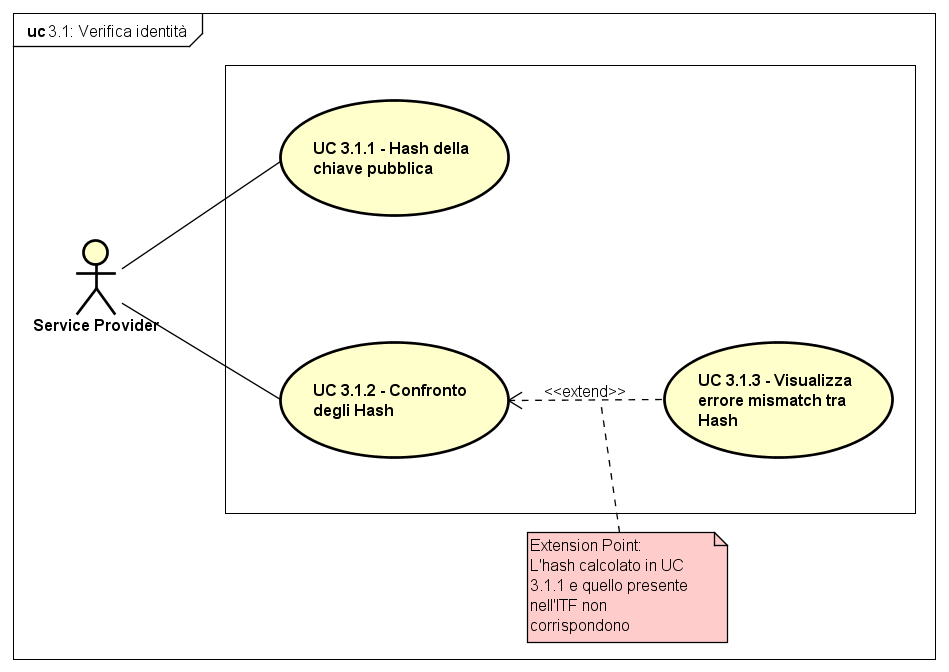
\includegraphics[scale=0.50]{immagini/usecase/UC31_VerificaIdentita}
	\caption{Caso d'uso UC3: Verifica}
\end{figure}
\begin{itemize}
	\item \textbf{Descrizione} - Il Service Provider, prima di poter erogare i suoi servizi, deve accertarsi che l'utente sia in possesso delle credenziali e degli attributi necessari. Questo avviene tramite la verifica dell'identità e la verifica degli attributi presenti nell'\gls{ITF};
	\item \textbf{Attori Principali} -Service Provider;
	\item \textbf{Attori Secondari} -
	\item \textbf{Pre-Condizioni} - Il Service Provider non ha verificato l'identità e gli attributi dell'utente;
	\item \textbf{Post-Condizioni} - Il Service Provider ha verificato l'identità dell'utente e può erogare i suoi servizi;
	\item \textbf{Scenario Principale} -
	\begin{enumerate}
		\item Verifica dell'identità dell'utente (UC 3.1);
		\item Verfica degli attributi dell'utente (UC 3.2).
	\end{enumerate}
	\item \textbf{Estensioni} -
	\begin{enumerate}
		\item Visualizza errore nella verifica dell'identità (UC 3.3);
		\item Visualizza errore nella verifica degli attributi (UC 3.4).
	\end{enumerate}
\end{itemize}
\subsection{Caso d'uso UC3.1: Verifica identità}
\begin{figure}[h]
	\centering
	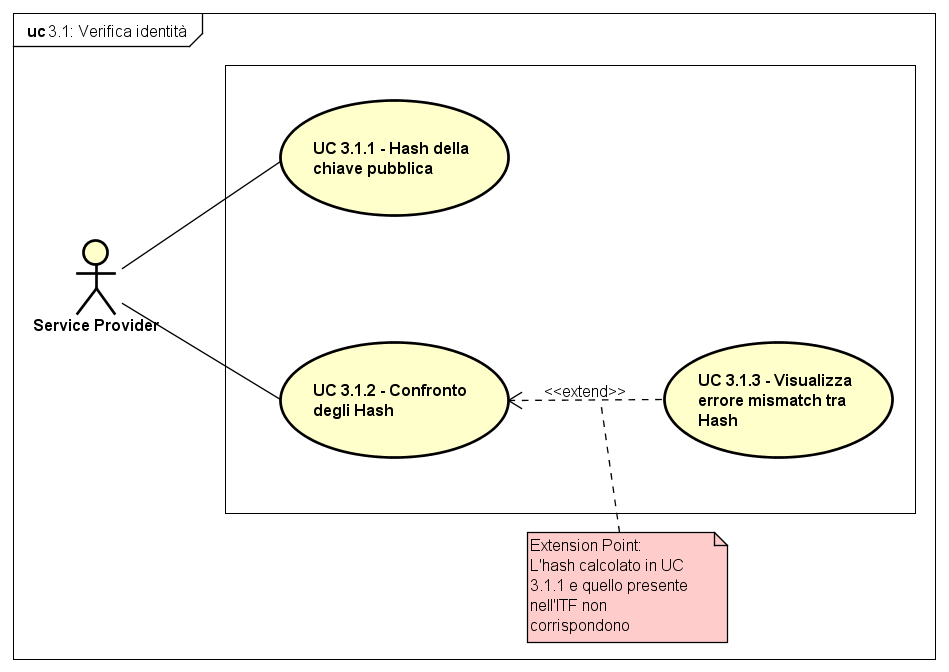
\includegraphics[scale=0.50]{immagini/usecase/UC31_VerificaIdentita}
	\caption{Caso d'uso UC3.1: Verifica dell'identità}
\end{figure}
\begin{itemize}
	\item \textbf{Descrizione} -  Il Service Provider, prima di permettere all'utente di usufruire dei suoi servizi, deve accertarsi che l'identità dell'utente sia corretta rispetto a quella presente nell'\gls{ITF};
	\item \textbf{Attori Principali} - Service Provider;
	\item \textbf{Attori Secondari} -
	\item \textbf{Pre-Condizioni} - L'attore non sa se può erogare i servizi all'utente;
	\item \textbf{Post-Condizioni} - Il Service Provider ha verificato l'identità dell'utente e può erogare i suoi servizi;
	\item \textbf{Scenario Principale} -
	\begin{enumerate}
		\item \textit{Hash} della chiave pubblica passata dall'Idenitity Wallet (UC 3.1.1);
		\item Confronto del \textit{hash} calcolato in UC 3.1.1 con quello presente nell'\gls{ITF} (UC 3.1.2).
	\end{enumerate}
	\item \textbf{Estensioni} -
	\begin{enumerate}
		\item Visualizza errore mismatch degli hash (UC 3.1.3).
	\end{enumerate}
\end{itemize}
\subsection{Caso d'uso UC3.3: Visualizza errore verifica dell'identità}
\begin{itemize}
	\item \textbf{Descrizione} - Il Service Provider, prima di poter erogare i suoi servizi, deve verificare che l'identità utente sia certificata e quindi presente nell'\gls{ITF}.\\
	Se questo non avviene, allora il Service Provider, non deve erogare nessun servizio all'utente che li richiede.\\
	Specificato meglio in caso d'uso UC3.1.3;
	\item \textbf{Attori Principali} - Service Provider;
	\item \textbf{Attori Secondari} -
	\item \textbf{Pre-Condizioni} - Il Service Provider è in attesa della verifica delle informazioni utente per erogare i suoi servizi;
	\item \textbf{Post-Condizioni} - Il Service Provider non è riuscito a verificare l'identità utente;
	\item \textbf{Scenario Principale} -
	\begin{enumerate}
		\item Viene visualizzato un errore di verifica dell'identità (UC 3.3).
	\end{enumerate}
	\item \textbf{Estensioni} -
\end{itemize}
\subsection{Caso d'uso UC3.1.3: Visualizza errore mismatch degli hash}
\begin{itemize}
	\item \textbf{Descrizione} - Il Service Provider, prima di poter erogare i suoi servizi, deve verificare che l'identità dell'utente sia corretta. Questo viene fatto tramite confronto degli \textit{hash}.\\
	Gli \textit{hash} da confrontare sono: quello presente nell'\gls{ITF} (certificato) e quello calcolato a partire dalla chiave pubblica che il Service Provider ha ottenuto dall'Identity Wallet.\\
	Se i due \textit{hash} non sono uguali significa che quello ottenuto dall'Identity Wallet non è corretto. Questo viene segnalato tramite un opportuno messaggio d'errore;
	\item \textbf{Attori Principali} - Service Provider
	\item \textbf{Attori Secondari} -
	\item \textbf{Pre-Condizioni} - L'attore è in attesa della verifica delle informazioni utente per erogare i suoi servizi;
	\item \textbf{Post-Condizioni} - L'attore, non essendo riuscito a verificare l'identità dell'utente, non può erogare i suoi servizi;
	\item \textbf{Scenario Principale} - 
	\begin{enumerate}
		\item Visualizza un opportuno errore di mismatch tra gli \textit{hash} delle chiavi pubbliche (UC 3.1.3).
	\end{enumerate}
	\item \textbf{Estensioni} -
\end{itemize}
\subsection{Caso d'uso UC3.4: Visualizza errore verifica degli attributi}
\begin{itemize}
	\item \textbf{Descrizione} - Il Service Provider deve, per poter erogare i suoi servizi, verificare l'identità e gli attributi dell'utente.\\
	L'identità viene spiegata in UC3.1, UC3.3 e in UC3.1.3.\\
	In questo caso, si ha come precondizione che l'identità sia stata verificata.
	Per poter erogare i servizi, il Service Provider, deve assicurarsi che l'utente sia in possesso degli attributi necessari che ne permettono l'autorizzazione all'utilizzo.\\
	Questo viene fatto andando a confrontare una lista di attributi, richiesti dal Service Provider, con la lista di attributi associati all'utente presente nell'\gls{ITF}.\\
	Essendo presente nell'\gls{ITF} vuol dire che la lista è composta solo da attributi certificati da una terza parte fidata.\\
	Se gli attributi richiesti dal Service Provider non son presenti, del tutto o in parte, nella lista degli attributi certificati dell'utente, il Service Provider non eroga nessun servizio;
	\item \textbf{Attori Principali} - Service Provider;
	\item \textbf{Attori Secondari} -
	\item \textbf{Pre-Condizioni} - Il Service Provider ha verificato correttamente l'identità dell'utente ma non sa se è in possesso degli attributi necessari per poter accedere ai suoi servizi;
	\item \textbf{Post-Condizioni} - Il Service Provider non è riuscito a verificare gli attributi dell'utente quindi non può erogare i suoi servizi in quanto non è autorizzato ad accedervi;
	\item \textbf{Scenario Principale} -
	\begin{enumerate}
		\item Visualizza un opportno messaggio d'errore per la verifica degli attributi (UC 3.4).
	\end{enumerate}
	\item \textbf{Estensioni} -
\end{itemize}
\subsection{Caso d'uso UC4: Aggiornamento}
\begin{figure}[h]
	\centering
	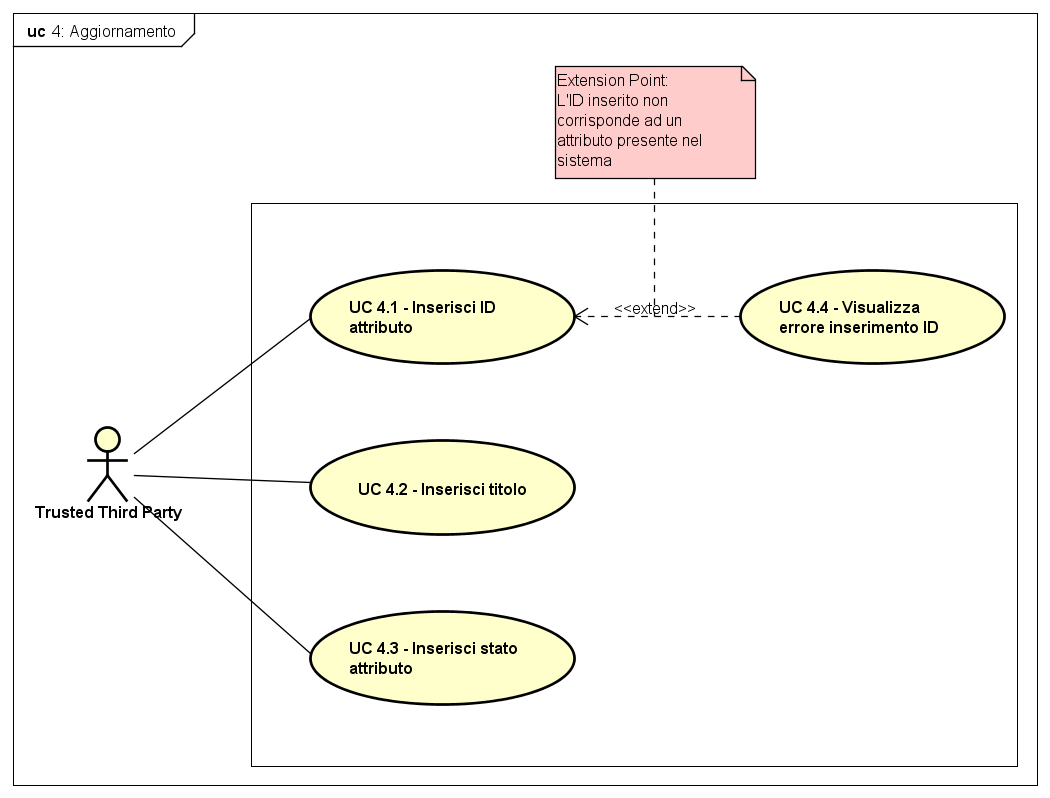
\includegraphics[scale=0.50]{immagini/usecase/UC4_Aggiornamento}
	\caption{Caso d'uso UC4: Aggiornamento}
\end{figure}
\begin{itemize}
	\item \textbf{Descrizione} -La Trusted Third Party, su richiesta dell'utente o non, deve aggiornare lo stato di un attributo o asserzione dell'utente stesso.
	Questo viene fatto creando un nuovo blocco che rappresenta l'attributo della quale si vuole fare l'aggiornamento. In questo nuovo blocco vengono inseriti: l'ID del vecchio blocco che si vuole aggiornare, la nuova descrizione dell'attributo e lo stato dell'attributo (ovvero se l'attributo è valido, se è all'ultima versione disponibile ecc..).\\
	Una volta creato il blocco verrà aggiunto un timestamp ed il nuovo blocco aggiunto alla catena.\\
	Quando un Service Provider vuole recuperare le informazioni riguardanti l'utente dovrà prendere il blocco con timestamp più recente. Questo tipo di aggiornamento fa sì che i nuovi blocchi "oscurino" quelli vecchi.\\
	I vecchi blocchi son comunque recuperabili grazie al riferimento che i nuovi blocchi hanno verso di loro. Questo permette la realizzazione di uno storico delle certificazioni prese da un utente e dello stato di avanzamento del \textit{Trust} che un utente ha nei confronti della rete;
	\item \textbf{Attori Principali} - Trusted Third Party;
	\item \textbf{Attori Secondari} -
	\item \textbf{Pre-Condizioni} - La Trusted Third Party vuole o deve, su richiesta dell'utente, aggiornare lo stato di un attributo che ha già certificato;
	\item \textbf{Post-Condizioni} - La Trusted Third Party è riuscita ad aggiornare lo stato di un attributo già certificato ;
	\item \textbf{Scenario Principale} -
	\begin{enumerate}
		\item Inserimento ID dell'attributo da aggiornare (UC 4.1);
		\item Inserimento del nuovo titolo descrittivo (UC 4.2);
		\item Inserimento dello stato del nuovo attributo (UC 4.3).
	\end{enumerate}
	\item \textbf{Estensioni} -
	\begin{enumerate}
		\item VIsualizza errore nell'inserimento ID (UC 4.4).
	\end{enumerate}
\end{itemize}
\subsection{Caso d'uso UC4.4: VIsualizza errore inserimento ID}
\begin{itemize}
	\item \textbf{Descrizione} - La Trusted Third Party deve, su richiesta dell'utente o per sua volontà, aggiornare lo stato di una certificazione.\\
	Questo avviene inserendo l'ID della certificazione che si vuole aggiornare ed aggiornando il titolo e lo stato. In automatico verrà posto un timestamp più recente che andrà ad "oscurare" le certificazioni meno recenti.\\
	L'errore viene scatenato quando si tenta di aggiornare un attributo che non esiste o non è presente nel sistema (ID errato);
	\item \textbf{Attori Principali} - Trusted Third Party;
	\item \textbf{Attori Secondari} -
	\item \textbf{Pre-Condizioni} - La Trusted Third Party vuole o deve, su richiesta dell'utente, aggiornare lo stato di un attributo che ha già certificato;
	\item \textbf{Post-Condizioni} - La Trusted Third Party non è riuscita ad aggiornare lo stato dell'attributo richiesto;
	\item \textbf{Scenario Principale} -
	\begin{enumerate}
		\item Visualizza errore inserimento ID (UC 4.4).
	\end{enumerate}
	\item \textbf{Estensioni} -
\end{itemize}
\subsection{Caso d'uso UC5: Revoca}
\begin{figure}[h]
	\centering
	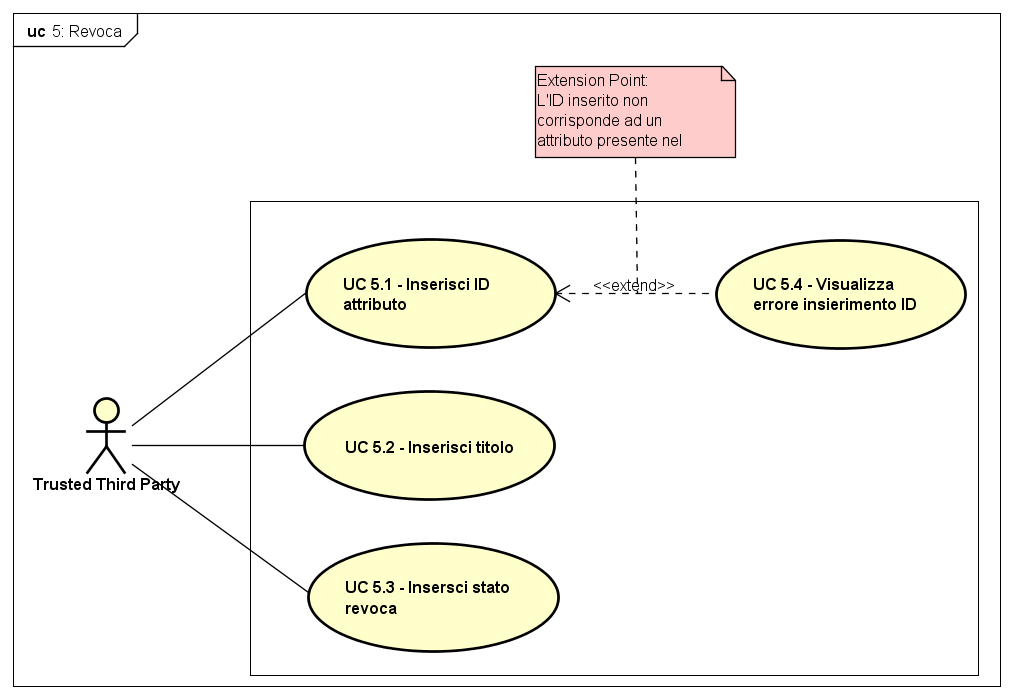
\includegraphics[scale=0.50]{immagini/usecase/UC5_Revoca}
	\caption{Caso d'uso UC5: Revoca}
\end{figure}
\begin{itemize}
	\item \textbf{Descrizione} - La Trusted Third Party può decidere di revocare una certificazione o un attributo che prima aveva certificato. Questo può avvenire per scadenza della certificazione o per ritiro da parte di enti terzi.\\
	Le dinamiche sono le stesse dell'aggiornamento (caso d'uso UC4) con la differenza che, lo stato viene utilizzato per indicare se un attributo è ancora valido o meno.\\
	Anche in questo caso il nuovo blocco inserito andrà ad "oscurare" tutti i blocchi con un timestamp più vecchio e sarà il Service Provider a dover recuperare i blocchi con timestamp più recente.\\
	Come nell'aggiornamento del UC4, anche qui è possibile ottenere uno storico delle certificazioni così da poter visualizzare il loro stato di avanzamento fino alla loro revoca;
	\item \textbf{Attori Principali} - Trusted Third Party;
	\item \textbf{Attori Secondari} -
	\item \textbf{Pre-Condizioni} - La Trusted Third Party deve revocare una particolare certificazione di un utente specifico;
	\item \textbf{Post-Condizioni} - La Trusted Third Party è riuscita a revocare la certificazione richiesta;
	\item \textbf{Scenario Principale} -
	\begin{enumerate}
		\item Inserimento dell'ID dell'attributo da rimuovere (UC 5.1);
		\item Inserimento del titolo dell'attributo da rimuovere (UC 5.2);
		\item Inserimento dello stato della revoca (UC 5.3).
	\end{enumerate}
	\item \textbf{Estensioni} -
	\begin{enumerate}
		\item Visualizza errore nell'inserimento dell'ID (UC 5.4).
	\end{enumerate}
\end{itemize}
\subsection{Caso d'uso UC5.4: Visualizza messaggio d'errore inserimento ID}
\begin{itemize}
	\item \textbf{Descrizione} - La Trusted Third Party deve revocare una certificazione.\\
	Questo avviene inserendo l'ID della certificazione che si vuole revocare ed inserendo un codice prefissato nello stato. In automatico verrà posto un timestamp più recente che andrà ad "oscurare" le certificazioni meno recenti.\\
	L'errore viene scatenato quando si tenta di revocare un attributo che non esiste o non è presente nel sistema (ID errato);	
	\item \textbf{Attori Principali} - Trusted Third Party;
	\item \textbf{Attori Secondari} -
	\item \textbf{Pre-Condizioni} - La Trusted Third Party deve revocare una certificazione sepcifica dell'utente;
	\item \textbf{Post-Condizioni} - La Trusted Third Party non è riuscita a revocare la certificazione dell'utente;
	\item \textbf{Scenario Principale} -
	\begin{enumerate}
		\item Visualizza errore inserimento ID (UC 5.4).
	\end{enumerate}
	\item \textbf{Estensioni} -
\end{itemize}
\section{Requisiti}
In questa sezione verranno elencati e descritti tutti i requisiti rilevati durante la fase di analisi dei requisiti. Questi saranno inseriti all'interno di una tabella contenente:
\begin{itemize}
	\item ID del requisito;
	\item Breve descrizione del requisito;
	\item Fonti dov'è possibile trovare o ricondursi al requisito stesso.
\end{itemize}
Prima di questo, verrà spiegata la nomenclatura adottata al fine di catalogare, ordinare e tracciare tutti i requisiti.
\subsection{Classificazione dei requisiti}
Ogni requisito viene calssificato secondo la seguente convenzione:\\
\centerline{R[Tipologia][Importanza]][Padre].[Livello]}\\
\begin{itemize}
	\item \textbf{Tipologia} - Indica la tipologia del requisito indicata con una lettera tra:
	\begin{itemize}
		\item \textbf{F}: \textit{Funzionale} ovvero le funzionalità che il sistema offre;
		\item \textbf{P}: \textit{Prestazionale} ovvero i vincoli sulle prestazioni che il sistema deve soddisfare;
		\item \textbf{Q}: \textit{Qualità} ovvero specifica i vincoli di qualità che il sistema deve soddisfare;
		\item \textbf{V}: \textit{Vincolo} ovvero rappresenta tutti i vincoli non funzionali che dipendono da fattori esterni, legali e di dominio.
	\end{itemize}
	\item \textbf{Importanza} - Indica l'importanza del requisito o la sua utilità strategica. Viene rappresentata da una lettera maiuscola tra:
	\begin{itemize}
		\item \textbf{O}: Rappresenta un requisito \textit{Obbligatorio} che deve essere soddisfatto per garantire le funzionalità base del sistema;
		\item \textbf{D}: Rappresenta un requisito \textit{Desiderabile} il cui non soddisfacimento non pregiudica le funzionalità del sistema ma, la sua realizzazione, da un valore aggiunto rendendo il tutto più completo;
		\item \textbf{F}: Rappresenta un requisito \textit{Facoltativo} che, se soddisfatto, renderebbe il sistema ancora più vompleto a discapito di risorse e aumento dei potenziali costi.
	\end{itemize}
	\item \textbf{Padre} - Numero che rappresenta univocamente un requisito;
	\item \textbf{Livello} - Per ogni "padre" il livello indica il numero del sotto requisito del caso preso in esame.
\end{itemize}
\subsection{Requisiti Funzionali}
\begin{longtable}{|r l|p{10cm}|p{2cm}|}
	\hline
	\multicolumn{2}{|c|}{\textbf{ID Requisito}} & \textbf{Descrizione} & \textbf{Fonti}\tabularnewline
	\hline
	&\textbf{RFO1.0}&Il sistema richiede che l'identità digitale venga generata&UC1 \\\hline
	&\textbf{RFO2.0}&Il sistema richiede la generazione delle chiavi pubbliche&UC1, UC1.1 \\\hline
	&\textbf{RFO3.0}&Il sistema richiede la generazione delle chiavi private&UC1, UC1.1 \\\hline
	&\textbf{RFO4.0}&Il sistema richiede l'inserimento delle informazioni personali dell'utente&UC1, UC1.2, UC1.2.1, UC1.2.2 \\\hline
	&\textbf{RFO4.1}&Il sistema richiede l'inserimento dei dati personali utente&UC1, UC1.2, UC1.2.1 \\\hline
	&\textbf{RFO4.1.1}&Il sistema richiede l'inserimento di un idetificativo&UC1.2, UC1.2.1 \\\hline
	&\textbf{RFO4.1.2}&Il sistema richiede l'inserimento della data di nascita&UC1.2, UC1.2.1 \\\hline
	&\textbf{RFO4.1.3}&Il sistema richiede l'inserimento del sesso ("M" per maschio o "F" per femmina)&UC1.2, UC1.2.1\\\hline
	&\textbf{RFO4.1.4}&Il sistema richiede l'inserimento del nome da associare all'identità digitale&UC1.2.1, UC1.2.1.1\\\hline
	&\textbf{RFO4.1.5}&Il sistema richiede l'inserimento del cognome da associare all'identità digitale&UC1.2.1, UC1.2.1.2\\\hline
	&\textbf{RFO4.2}&Il sistema richiede l'inserimento degli attributi associati all'utente&UC1, UC1.2, UC1.2.2 \\\hline
	&\textbf{RFO4.2.1}&Il sistema richiede l'inserimento di un identificativo per l'attributo&UC1.2.2, UC1.2.2.1 \\\hline
	&\textbf{RFO4.2.1.1}& L'identificativo associato all'attributo deve essere univoco&UC1.2.2, UC1.2.2.1 \\\hline
	&\textbf{RFO4.2.2}&Ad ogni attributo va associato un titolo che lo descrive&UC1.2.2, UC1.2.2.2 \\\hline
	&\textbf{RQD1}& & \\\hline
	&\textbf{RQD1}& & \\\hline
	&\textbf{RQD1}& & \\\hline
	&\textbf{RQD1}& & \\\hline
	&\textbf{RQD1}& & \\\hline
	&\textbf{RQD1}& & \\\hline
	&\textbf{RQD1}& & \\\hline
	&\textbf{RQD1}& & \\\hline
	&\textbf{RQD1}& & \\\hline
	&\textbf{RQD1}& & \\\hline
	&\textbf{RQD1}& & \\\hline
	&\textbf{RQD1}& & \\\hline
	&\textbf{RQD1}& & \\\hline
	&\textbf{RQD1}& & \\\hline
	&\textbf{RQD1}& & \\\hline
	&\textbf{RQD1}& & \\\hline
	&\textbf{RQD1}& & \\\hline
	&\textbf{RQD1}& & \\\hline
	&\textbf{RQD1}& & \\\hline
	&\textbf{RQD1}& & \\\hline
	&\textbf{RQD1}& & \\\hline
	&\textbf{RQD1}& & \\\hline
	&\textbf{RQD1}& & \\\hline
	&\textbf{RQD1}& & \\\hline
	&\textbf{RQD1}& & \\\hline
	&\textbf{RQD1}& & \\\hline
	&\textbf{RQD1}& & \\\hline
	&\textbf{RQD1}& & \\\hline
	&\textbf{RQD1}& & \\\hline
	&\textbf{RQD1}& & \\\hline
	&\textbf{RQD1}& & \\\hline
	&\textbf{RQD1}& & \\\hline
	&\textbf{RQD1}& & \\\hline
	&\textbf{RQD1}& & \\\hline
	&\textbf{RQD1}& & \\\hline
	&\textbf{RQD1}& & \\\hline
	&\textbf{RQD1}& & \\\hline
	&\textbf{RQD1}& & \\\hline
	&\textbf{RQD1}& & \\\hline
	\caption{Tabella requisiti funzionali}
\end{longtable}
\subsection{Requisiti di Qualità}
Tramite i requisiti di qualità si vogliono indicare quelle caratteristiche che un \gls{ITF} dovrebbe riuscire a raggiungere in modo da garantire un certo livello di \textit{Trust} del sistema.\\
Per una migliore spiegazione si rimanda al documento "Blockchain: The Dawn of Decentralized Identity"\cite{ITF_gartner} dalla quale son stati presi tutti i requisiti di qualità che verranno elencati.
\begin{longtable}{|r l|p{10cm}|p{2cm}|}
	\hline
	\multicolumn{2}{|c|}{\textbf{ID Requisito}} & \textbf{Descrizione} & \textbf{Fonti}\tabularnewline
	\hline
	&\textbf{RQD1}&Il sistema deve garantire un certo livello di\textit{Trust} (Fiducia)& Capitolo 2, Doc.Gartner\cite{ITF_gartner}\\\hline
	&\textbf{RQD2}&Il sistema deve garantire un certo livello di \textit{Assurance} (Garanzia)& Capitolo 2, Doc.Gartner\cite{ITF_gartner}\\\hline
	&\textbf{RQD3}&Il sistema deve garantire un certo livello di \textit{Provenance} (Provenienza delle informazioni)& Capitolo 2, Doc.Gartner\cite{ITF_gartner}\\\hline
	&\textbf{RQD4}&Il sistema deve garantire un certo livello di \textit{Security} (Sicurezza)& Capitolo 2, Doc.Gartner\cite{ITF_gartner}\\\hline
	&\textbf{RQD5}&Il sistema deve garantire un certo livello di \textit{Scalability} (Scalabilità)& Capitolo 2, Doc.Gartner\cite{ITF_gartner}\\\hline
	&\textbf{RQD6}&Il sistema deve garantire un certo livello di \textit{Efficency} (Efficenza)& Capitolo 2, Doc.Gartner\cite{ITF_gartner}\\\hline
	\caption{Tabella requisiti di qualità}
\end{longtable}
\subsection{Requisiti di Vincolo}
\begin{longtable}{|r l|p{10cm}|p{2cm}|}
	\hline
	\multicolumn{2}{|c|}{\textbf{ID Requisito}} & \textbf{Descrizione} & \textbf{Fonti}\tabularnewline
	\hline
	&\textbf{RVO1}& La piattaforma Blockchain utilizzata sarà Ethereum & Capitolo 2\\\hline
	&\textbf{RVO1.1}& Per lo sviluppo della rete Blockchain verrà utilizzato il \gls{framework} \textit{Truffle suite} & Capitolo 2\\\hline
	&\textbf{RVO2}& Per lo sviluppo degli \textit{smart contracts} il linguaggio utilizzato sarà Solidity (versione 0.4.24 o superiore) & Capitolo 2\\\hline
	&\textbf{RVO3}& Il sistema deve funzionare con il sistema operativo Windows 10 & Capitolo 2\\\hline
	&\textbf{RVO4}& Per lo sviluppo della rete Blockchain verrà utilizzato il tool \textit{Ganache} & Capitolo 2\\\hline
	\caption{Tabella reqisiti di vincolo}
\end{longtable}
\subsection{Riepilogo dei requisiti}             % Kick-Off
% !TEX encoding = UTF-8
% !TEX TS-program = pdflatex
% !TEX root = ../tesi.tex

%**************************************************************
\chapter{Progettazione}
\label{cap:progettazione}
%**************************************************************
In questo capitolo viene esposta una panoramica dell'architettura adottata per la realizzazione del modulo \gls{ITF} comprensiva di un analisi sulla scelta architetturale. Segue, poi, la trattazione della progettazione del modulo vero e proprio.\\
\section{Descrizione Architetturale}
Durante lo sviluppo del modulo \gls{ITF} mi è stata data piena libertà nella scelta dello stile architetturale da adottare. Per questo motivo, dopo un breve periodo di analisi e studio dei vari stili possibili, la scelta è ricaduta su un'architettura \textit{Layered 3-tier}.\\
Di seguito verrà presentata una panoramica generale di come funziona lo stile architetturale scelto insieme all'analisi dei suoi punti di forza e debolezza. Per quanto riguarda questi ultimi vengono anche discusse possibili soluzioni.\\
\subsection{Stile architetturale}
\begin{figure}[h]
	\centering
	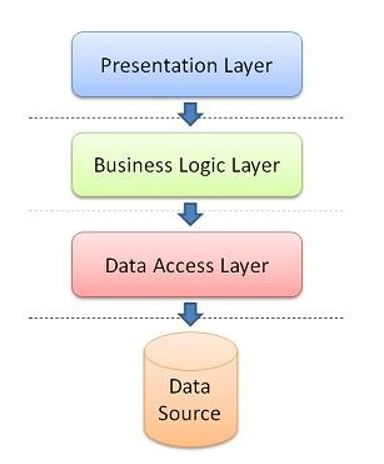
\includegraphics[scale=1]{immagini/layered_architecture}
	\caption{Schema architettura Layered 3-tier}
\end{figure}
L'architettura \textit{Layered 3-tier} è un architettura software molto semplice in cui le varie funzionalità sono separate logicamente ovvero suddivise su livelli logici differenti in comunicazione tra di loro.\\
I componenti all'interno di un'architettura di questo tipo sono organizzati in livelli orizzontali, ognuno dei quali si occupa di uno specifico ruolo all'interno del sistema completo.\\
Il pattern di questa tipologia di architettura non specifica il numero di livelli ma, nella versione più comune, il numero di livelli è tre suddiviso in: \textit{Presentation Layer}, \textit{Business Logic Layer} e \textit{Data Access Layer} il quale, poi, si occuperà di accedere ai dati all'interno del \textit{Data Source}.\\
Ogni livello, come abbiamo già visto, si occupa di uno specifico ruolo all'interno del sistema completo:
\begin{itemize}
	\item \textbf{Presentation Layer} - ha lo scopo di gestire l'interazione del sistema con il mondo esterno, in particolare con gli utenti. Include le maschere per visualizzare e inserire dati, controlli, dai più semplici ai più complessi, e i meccanismi per intercettare e gestire opportunamente tutti gli eventi che sono scatenati dalle azioni degli utenti;
	\item \textbf{Business Logic Layer} - include l'insieme delle regole di business che regolano il funzionamento dell'applicazione, intercetta le richieste provenienti dallo strato di presentazione e le gestisce opportunamente;
	\item \textbf{Data Access Layer} - conosce le modalità per leggere e salvare le informazioni interne al sistema nell'ambito di una sorgente dati (non necessariamente un database centralizzato).
\end{itemize}
\subsection{Analisi e rating dell'architettura scelta}
La seguente tabella contiene una valutazione delle principali caratteristiche dell'architettura scelta.\\
Andremo ora a spiegarle e ad analizzarle.
\begin{figure}[h]
	\centering
	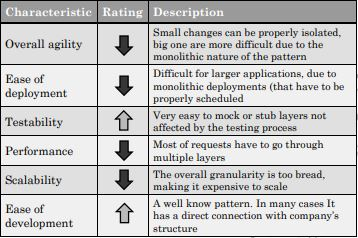
\includegraphics[scale=1]{immagini/layered_architecture_analysis}
	\caption{Analisi dell'architettura Layered 3-tier}
\end{figure}
\begin{itemize}
	\item \textbf{Overall agility}:
	\begin{itemize}
		\item \textbf{Rating}: Basso;
		\item \textbf{Analisi}: è la capacità del sistema di reagire velocemente ad un ambiente in costante cambiamento. Nonostante le modifiche siano essere isolate attraverso i livelli è comunque difficile apportare dei cambiamenti a causa della sua struttura monolitica della maggior parte delle implementazioni che lo adottano e dello stretto accoppiamento che si ha tra i livelli\cite{3tierArch}\cite{3tierArch2}.
		\item \textbf{Valutazione}: nonostante la non semplice gestione dei cambiamenti questo non è un problema per lo sviluppo del modulo \gls{ITF} in quanto, essendo il sistema sviluppato interamente appoggiandosi ad \textit{Ethereum}, le modifiche sono difficili di per sé a causa dell'immutabilità garantita ai contratti una volta che questi sono rilasciati nella rete.\\
		Per andare a modificare un contratto, l'unico modo è riscriverlo con tutte le modifiche necessarie e sostituire gli indirizzi nei contratti che lo utilizzano.\\
		Potrebbe risultare un procedimento complesso ma così non è se si adottano strategie che prevedono questo scenario (metodi di \textit{setting} degli indirizzi bloccati ai soli proprietari dei contrati).\\
	\end{itemize}
	Per questa motivazione nonostante il rating basso di questa caratteristica, il sistema non ne viene influenzato in modo negativo.
	\item \textbf{Ease of deployment}:
	\begin{itemize}
		\item \textbf{Rating}: Basso;
		\item \textbf{Analisi}: un piccolo cambiamento ad una componente può richiedere la ri-implementazione dell'intera applicazione o di una grossa porzione di essa, facendo sì che sia necessaria la pianificazione e l'implementazione durante ore non lavorative\cite{3tierArch}\cite{3tierArch2}.
		\item \textbf{Valutazione}: come per l'\textit{Overall agility} questa caratteristica non è un problema per l'implementazione del modulo se viene pensato per essere estesto in quanto, come detto nel punto precedente, essento tutto appoggiato sopra la rete \textit{Ethereum} l'implementazione di nuovi contratti o la loro modifica necessità la creazione del contratto e la sostituzione degli indirizzi all'interno dei contratti che lo utilizzano.
	\end{itemize}
	\item \textbf{Testability}:
	\begin{itemize}
		\item \textbf{Rating}: Alto;
		\item \textbf{Analisi}: siccome i componenti sono suddivisi in livelli separati è possibile creare dei mockup o degli \emph{\gls{stub}}\glsfirstoccur per i livelli che dipendono direttamente da quello che si sta sviluppando. Questo fa sì che la testabilità del sistema sia molto facile\cite{3tierArch}\cite{3tierArch2}.\\
		\item \textbf{Valutazione}: essendo, la maggior parte del modulo, appoggiato ad \textit{Ethereum} ed essendo i contratti immutabili, una volta rilasciati nella rete, si ha la necessità di operare un gran numero di test prima del rilascio in modo da evitare di dover creare un nuovo contratto che va a sostituire quello contenente errori.\\
		Per questo motivo questa caratteristica è di fondamentale importanza per il modulo \gls{ITF}.		
	\end{itemize}
	Questa caratteristica è fondamentale per l'\gls{ITF} \textit{Ethereum} e il suo rating alto è stato uno dei motivi di scelta dell'intera architettura.
	\item \textbf{Performance}:
	\begin{itemize}
		\item \textbf{Rating}: Basso
		\item \textbf{Analisi}: il pattern architetturale non si presta bene nell'avere alte performance questo è dato dal fatto che ogni volta che si vuole interagire con un livello bisogna necessariamente passare attraverso multipli livello per andare a soddisfare la richiesta\cite{3tierArch}\cite{3tierArch2}.
		\item \textbf{Valutazione}: il fatto di dover passare attraverso molti livelli senza dare la possibilità di "scavalcarne" alcuni per determinate richieste è un concetto chiave dell'architettura detto T\textit{he layers of Isolation}. Questo fa sì che ogni cambiamento ad un livello non abbia effetto su altri componenti di altri livelli: il cambiamento è isolato ai componenti interni al livello.\\
		Se si permettesse ad alcuni componenti di "scavalcare" i livelli direttamente sottostanti, i cambiamenti a questo livello influenzerebbero pesantemente tutti gli altri andando a creare un forte accoppiamento tra le parti.\\
		La considerazione da fare è che, il sistema che vogliamo realizzare, è semplice e non prevede una profondità dei livelli così alta da andare a inficiare pesantemente sulle prestazioni del modulo in più c'è da dire che la \textit{Blockchain Ethereum} è il vero freno sulle prestazioni del sistema in quanto, una transazione, potrebbe richiedere anche svariati minuti.
	\end{itemize}
	\item \textbf{Scalability}:
	\begin{itemize}
		\item \textbf{Rating}: Basso
		\item \textbf{Analisi}: la Scalabilità (capacità di un sistema di reagire a richieste di lavoro più pesanti) è un problema per i sistemi sviluppati tramite l'utilizzo di questa architettura. In un'architettura di questo tipo la scalabilità può essere ottenuta andando a dividere i vari livelli in implementazioni fisicamente separate o andando a replicare l'interna applicazione in nodi multipli\cite{3tierArch}\cite{3tierArch2}.
		\item \textbf{Valutazione}: questa caratteristica potrebbe essere l'unica in grado di andare ad intaccare il modulo \gls{ITF} se non pensato correttamente.\\
		Secondo me, il problema principale all'interno della rete \textit{Ethereum} alla quale ci andiamo ad appoggiare, è principalmente dovuto alla scrittura dei dati e quindi durante la fase di registrazione di un nuovo utente o l'aggiornamento dei certificati conseguiti.\\
		Queste essendo operazioni che avvengono con bassa frequenza (un utente si registra una sola volta in quanto l'identità digitale è unica ma condivisa per ogni servizio e l'inserimento di nuove certificazioni non è un'operazione che viene fatta ) potrebbero non avere effetti negativi nel sistema in quanto, quello che viene fatto principalmente, sono letture di dati da parte dei vari Service Providers prima di permettere il rilascio di un servizio.
	\end{itemize}
	\item \textbf{Ease of development}:
	\begin{itemize}
		\item \textbf{Rating}: Alto
		\item \textbf{Analisi}: l'Ease of development (facilità di sviluppo) raggiunge livelli molto alti soprattutto data dal fatto che è un'architettura molto semplice e conosciuta.\\
		Siccome molte compagnie ed aziende sviluppano applicazioni e sistemi andando a separare i livelli per competenze, questo pattern diventa una delle scelte migliori\cite{3tierArch}\cite{3tierArch2}.
		\item \textbf{Valutazione}: la facilità di sviluppo di un sistema basato su questa architettura è, sicuramente, una caratteristica importante.\\
		Questo viene dal fatto che, grazie ad un'architettura del genere, è possibile andare a mettere le mani nel codice in tempi molto più brevi rispetto a quelli richiesti se venisse adotta un'altra tipologia di architettura.\\
		In più, il fatto di poter dividere i vari livelli per competenze permette lo sviluppo separato e parallelo di componenti diverse senza la necessità che il sistema segua un filo logico inizio – fine.\\
		Quest'ultimo accorgimento è di fondamentale importanza in quanto è stato necessario suddividere la parte fornt-end dal back-end e lo sviluppo è avvenuto in parallelo.
	\end{itemize}
\end{itemize}
\section{Approccio alla progettazione}
Per la progettazione del modulo si è deciso di utilizzare un approccio \emph{\gls{topDown}}\glsfirstoccur. Essa consiste nel descrivere il sistema partendo da una visione generale ad alto livello per poi scendere nel particolare delle parti individuate.\\
Nella visione ad alto livello è possibile notare che il sistema è composto da diversi packages che interagiscono tra di loro. Entrando nel dettaglio si vanno ad individuare tutte le componenti più piccole e semplici tramite la strategia \textit{divide-et-impera}. L'approccio \gls{topDown} parte dall’obiettivo e da esso valorizza il "perché" e fa dipendere il "come", permettendo di suddividere il lavoro rendendolo più comprensibile e, quindi, di più facile manutenibilità.
\section{Architettura generale}
Il modulo \gls{ITF} è formato da due parti distinte:
\begin{itemize}
	\item \textbf{Front-end}:l'applicativo tramite la quale gli utenti e gli attori esterni possono interagire con l'intero sistema;
	\item \textbf{Back-end}: tutte le componenti che contengono la \textit{Business Logic}, gestiscono la presistenza dei dati interni alla \textit{Blockchain Ethereum} e le componenti necessarie a far sì che il \textit{front-end} riesca ad interagire con la \textit{Business Logic}.
\end{itemize}
Il lato \textit{back-end} prevede l'utilizzo della \textit{Blockchain Ethereum} per la gestione e la certificazione delle informazioni personali dell'utente insieme alla verifica delle informazioni da parte di un Service Provider che ha ricevuto una richiesta di accesso da parte di un utente.\\
Tutte queste operazioni vengono gestite tramite \textit{smart contracts Solidity} in modo da permettere l'interazione con l'\gls{evm}.\\
Tutte le componenti della parte \textit{back-end} sono raggruppate in packages. Questo viene fatto perchè, all'interno di ogni package, troviamo:
\begin{itemize}
	\item Gli \textit{smart contracts} che contengono i dati da gestire e dei metodi fittizi che contengono gli indirizzi ai metodi veri e propri;
	\item Gli \textit{smart contracts} contenenti l'implementazione vera e propra dei vari metodi.
\end{itemize}
Questo è necessario in quanto un contratto \textit{Ethereum}, una volta rilasciato nella rete, diventa immutabile e quindi non più modificabile in caso di malfunzionamenti o risultati inaspettati.\\
Separando la parte logica (metodi) dalla componente dati (con metodi fittizi) e collegando le due parti tramite indirizzi fa sì che l'eventuale presenza di errori possa essere gestita andando a implementare nuovamente solo la parte logica e cambiando gli indirizzi nella componente dati (questo cambiamento deve essere gestito tramite appositi metodi \textit{setter}).
\newpage
\section{Componenti del modulo}
\subsection{Visione generale}
\begin{figure}[!h]
	\centering
	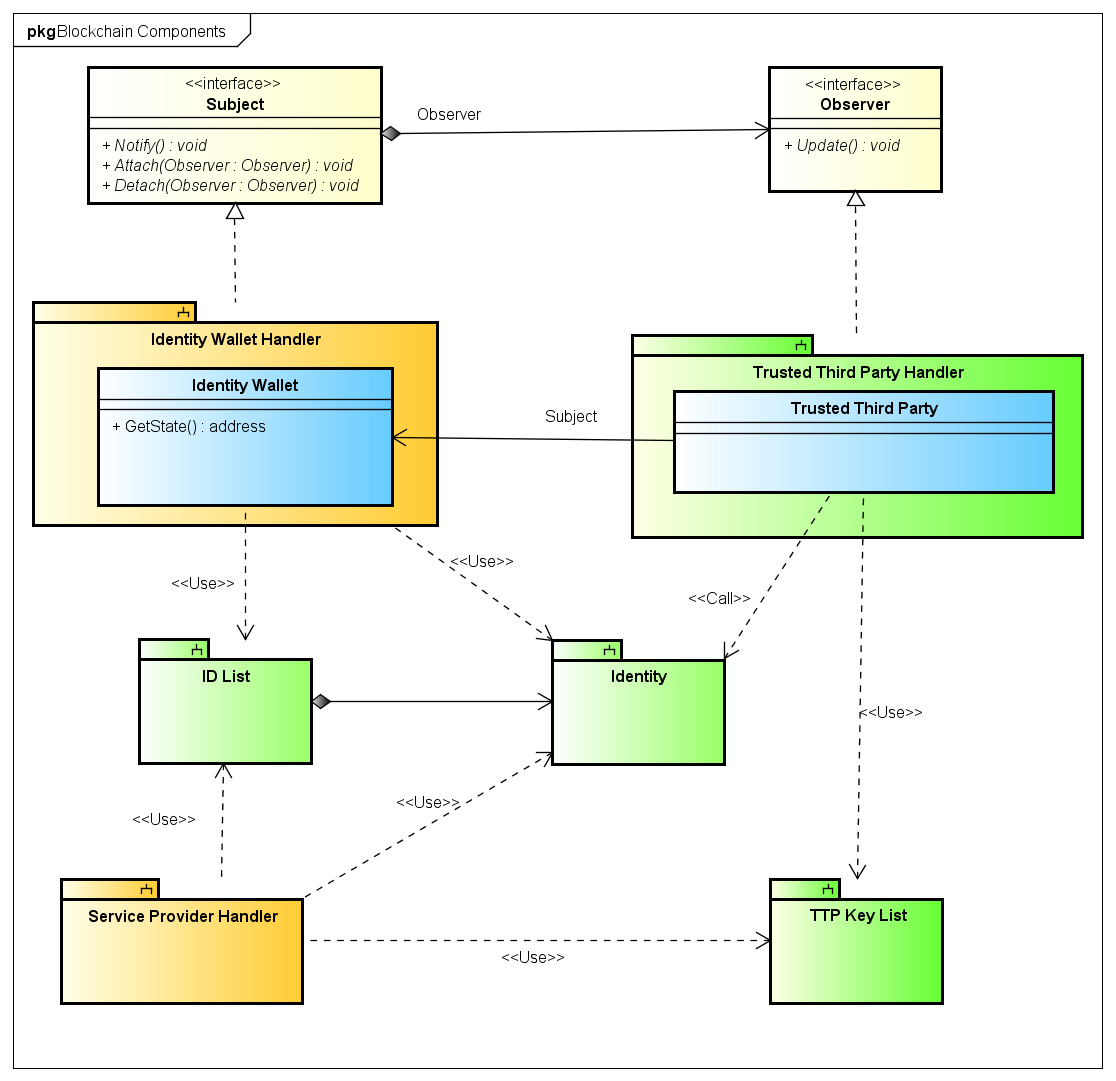
\includegraphics[scale=0.5]{immagini/architettura_alto_livello}
	\caption{Visione ad alto livello}
	\label{fig:visioneAltoLivello}
\end{figure}
\begin{itemize}
	\item \textbf{Descrizione}:\\
	Questo è il package principale dell'applicazione lato \textit{back-end}.\\
	Tutte le classi e i sottosistemi presenti in questo package contengono la \textit{business logic} e la persistenza dei dati necessari per realizzare il modulo \gls{ITF} e la sua interazione con il mondo esterno verso il Service Provider e l'Identity Wallet.
	\item \textbf{Package contenuti}:\\
	\begin{itemize}
		\item Identity Wallet Handler;
		\item Trusted Third Party;
		\item ID List;
		\item TTP Key List;
		\item Identity;
		\item Service Provider Handler.
	\end{itemize}	
\end{itemize}
Come si può vedere dallo schema in figura \ref{fig:visioneAltoLivello} le varie componenti presentano dei colori diversi. Questo è stato fatto per rendere più chiara la suddivisione dei package in base al \textit{design pattern} ad essi associati.\\
\begin{itemize}
	\item \textbf{Design pattern Observer} - formano questo design pattern: il package Identity Wallet Handler, la classe Trusted Third Party e le interfacce Subject e Observer (colore: azzurro);
	\item \textbf{Design pattern Façade} - formano questo design pattern i due package Service Provider Handler e Identity Wallet Handler (colore: arancione);
	\item \textbf{Desing pattern Strategy} - tutti i package nello schema presentano questo design pattern al loro interno quindi: Identity Wallet Handler, Service Provider Handler, ID List e Identity (colore verde).
\end{itemize}
Alcuni package non rispettano i colori sopracitati in quanto realizzano più di un design pattern. Vedremo in seguito quali.
\subsection{Identity Wallet Handler}
\begin{figure}[!h]
	\centering
	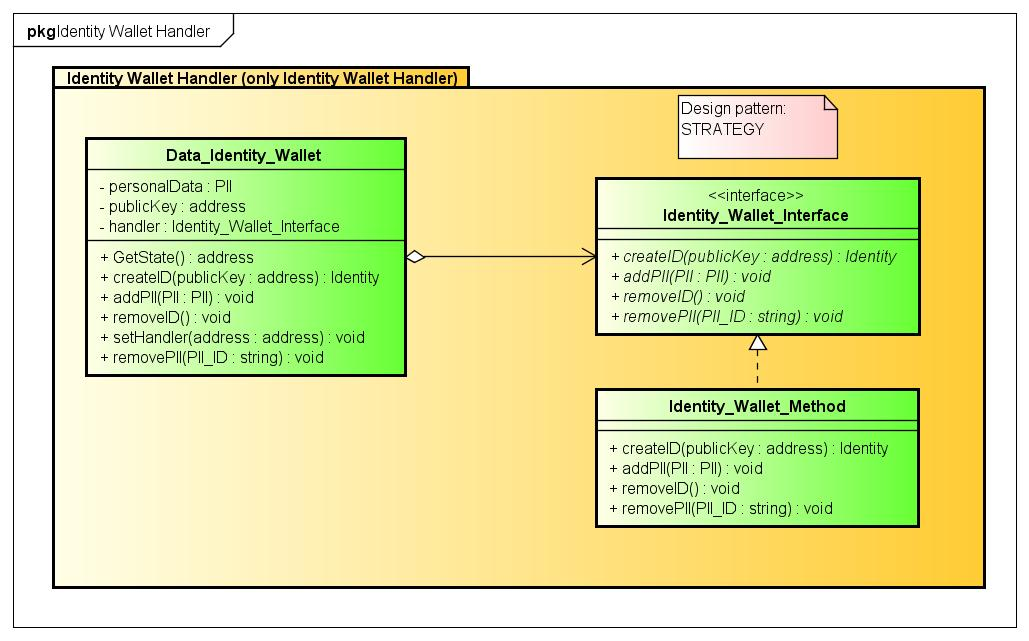
\includegraphics[width=0.8\textwidth]{immagini/identityWalletHandler}
	\caption{Schema Identity Wallet}
\end{figure}
\begin{itemize}
	\item \textbf{Descrizione}
	Package che modella l'interazione tra l'Identity Wallet ed il sistema esterno. Si occupa principalmente di tutte le attività che l'utente può fare all'interno della \textit{Blockchain Ethereum}.\\
	Contiene, al suo interno, tutte le classi necessarie affinché si riesca a mantenere separati le informazioni dai metodi.\\
	Il nome del package tra parentesi (only Identity Wallet Handler) è un modo per indicare la possibilità, che da \textit{Solidity}, di far eseguire le operazioni contenute in Data\_Identity\_Wallet solo dal Wallet stesso e non da altri contratti esterni.
	\item \textbf{Interazione con altre componenti}
	\begin{itemize}
		\item Trusted Third Party;
		\item ID List;
		\item Identity.
	\end{itemize}
	\item \textbf{Design pattern presenti}
	\begin{itemize}
		\item Façade (arancione);
		\item Strategy (verde);
		\item Singleton (non segnato);
		\item Observer (non segnato).
	\end{itemize}
\end{itemize}
\subsubsection{Data\_Identity\_Wallet}
\begin{itemize}
	\item \textbf{Descrizione}
	Componente che racchiude tutta l'essenza del package Identity Wallet Handler.
	Questa classe contiene metodi, informazioni riguardanti l'identità dell'utente e informazioni necessarie per l'interazione con il sistema.\\
	Per realizzare il modulo in \textit{Ethereum} è consigliato separare la \textit{business logic} e la persistenza dei dati. Questa componente mantiene principalmente tutti i dati necessari e delega, tramite \textit{strategy} pattern, la realizzazione dei metodi ad altre componenti.\\
	Il codice, se presenta dei bug o comportamenti anomali, non è possibile correggerlo. L'unico modo per risolvere è andare a rimpiazzare il vecchio contratto con uno nuovo e cambiare gli indirizzi dei client che utilizzavano il modulo precedente.\\
	Se la classe contenesse sia dati che metodi allora bisognerebbe rimpiazzare tutto il blocco perdendo così i dati degli utenti registrati.\\
	Separando la componente logica dai dati e collegando il tutto tramite pattern \textit{strategy} è possibile, in caso di errore, creare un nuovo Identity\_Wallet\_Method e, senza alcuna perdita di dati utente, ripristinare il normale funzionamento del modulo.	
	\item \textbf{Interazione con altre componenti}
	\begin{itemize}
		\item\textbf{ Identity\_Wallet\_Interface}: Questo contratto contiene la firma dei metodi che, le classi concrete che realizzano l'interfaccia, devono implementare per andare a soddisfare le richieste che vengono fatte dall'Identity Wallet tramite Data\_Identity\_Wallet.
		\item\textbf{ Identity\_Wallet\_Method}:Contratto che realizza le specifiche dell'interfaccia Identity\_Wallet\_Interface tramite l'implementazione concreta di tutti i metodi dichiarati.
	\end{itemize}
	\item \textbf{Design pattern presenti}\\
	Partecipa alla realizzazione del pattern \textit{strategy} interno al package Identity Wallet Handler e realizza, insieme alla classe Trusted Third Party, il design pattern \textit{Observer} necessario per la certificazione delle informazioni personali.
\end{itemize}
\subsection{ID List}
\begin{figure}[!h]
	\centering
	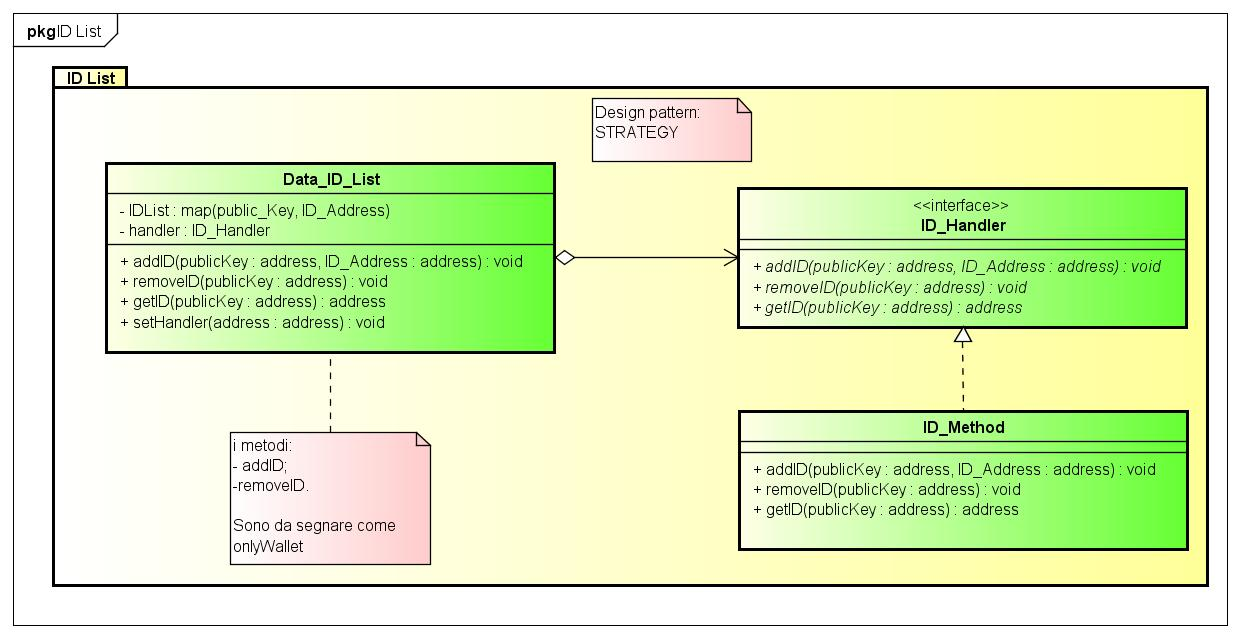
\includegraphics[width=0.8\textwidth]{immagini/idList}
	\caption{Schema ID List}
\end{figure}
\begin{itemize}
	\item \textbf{Descrizione}
	Package che fa da ponte tra le varie componenti interne al sistema. 
	Al suo interno contiene tutte le informazioni e i metodi necessari per far comunicare tra di loro l'Identity Wallet Handler, Trusted Third Party e Service Provider Handler.\\
	Come gli altri package, anche questo presenta il consueto \textit{strategy} pattern per separare la business logic e la persistenza dei dati.\\
	Un altro design pattern che questa componente realizza è il \textit{singleton} in quanto è utilizzata da tutte le altre componenti per recuperare le informazioni delle identità utente che essa contiene.\\
	Alcuni metodi di questo package sono segnati come onlyWallet ovvero con il permesso reso disponibile da \textit{Solidity} che fa sì che sia possibile specificare quale componente può invocare i metodi, rigettando le chiamate da tutti gli altri contratti non specificati.
	\item \textbf{Interazione con altre componenti}
	\begin{itemize}
		\item Identiy Wallet Handler;
		\item Identity;
		\item Trusted Third Party;
		\item Service Provider Handler.
	\end{itemize}
	\item \textbf{Design pattern presenti}\\
	Partecipa alla realizzazione del design pattern \textit{strategy} ed è un \textit{singleton} per recuperare tutte le informazioni riguardanti le identità digitali degli utenti.
\end{itemize}
\subsubsection{Data\_ID\_List}
\begin{itemize}
	\item \textbf{Descrizione}
	Rappresenta la componente principale di tutto il package ID List in quanto si occupa sia della gestione dei dati che dell'invocazione dei metodi.\\
	Questa componente si occupa principalmente di mantenere una mappatura tra l'identità dell'utente (rappresentata da un indirizzo \textit{Ethereum}) e la corrispondente identità nell'Identity Wallet (rappresentata da una chiave pubblica). Queste informazioni vengono conservate all'interno di una mappa che associa i due tipi di informazioni per ogni utente registrato al sistema.\\
	Oltre a questo, troviamo anche i metodi necessari per poter inserire, rimuovere e recuperare l'identità utente.\\
	Partecipando ad un design pattern \textit{strategy} i metodi interni a questa componente delegano l'esecuzione a ID\_Method in modo da preservare la separazione tra dati e business logic.
	\item \textbf{Interazione con altre componenti}
	\begin{itemize}
		\item \textbf{ID\_Handler}: Interfaccia necessaria per la realizzazione del pattern \textit{strategy} interno al package ID List.\\
		Contiene le firme di tutti i metodi che sono utilizzati da Data\_ID\_List e che sono realizzati, concretamente, dalla componente ID\_Method.
		\item \textbf{ID\_Method}: Classe che implementa i metodi necessari per recuperare, inserire ed eliminare le informazioni associate alle identità utente.\\
		Realizza, concretamente, tutti i metodi richiamati dal Data\_ID\_List ed esposti dall'interfaccia ID\_Handler.
	\end{itemize}
	\item \textbf{Design pattern presenti}\\
	Realizza il design pattern \textit{strategy} interno al package.
\end{itemize}
\subsection{Identity}
\begin{figure}[!h]
	\centering
	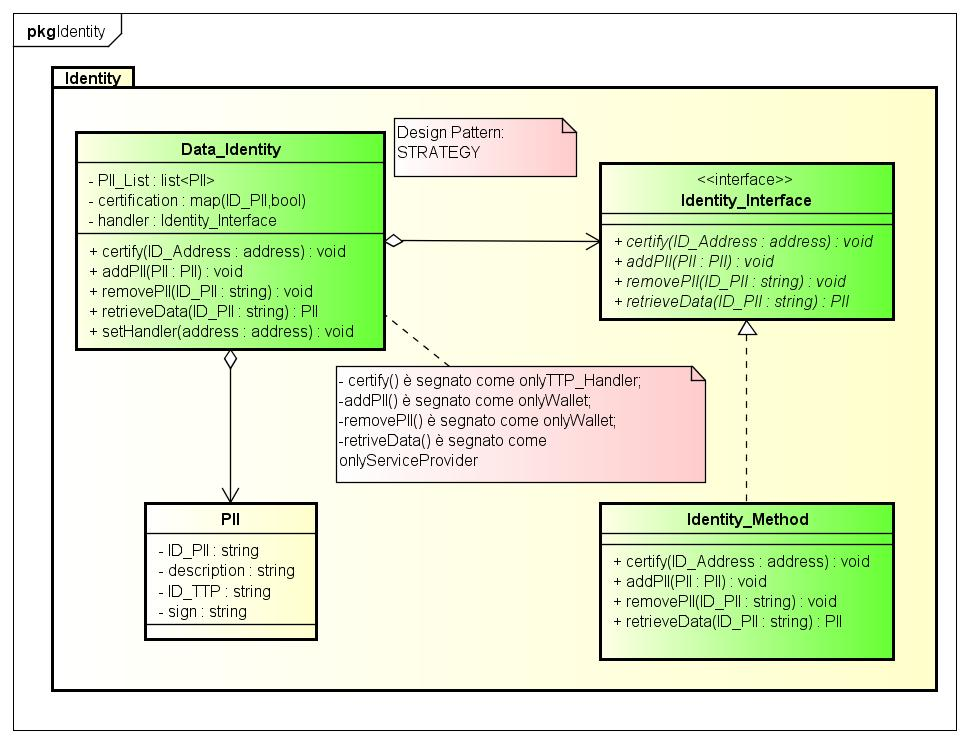
\includegraphics[width=0.8\textwidth]{immagini/identity}
	\caption{Schema Identity}
\end{figure}
\begin{itemize}
	\item \textbf{Descrizione}
	Package che contiene tutti i dati e le informazioni personali relative all'identità di un utente e tutti i metodi necessari, agli altri package, per poter aggiungere, rimuovere, certificare e verificare le \gls{PII}.\\
	Questo è un altro dei package core del sistema \gls{ITF} che si vuole realizzare in quanto, insieme all'Identity\_Wallet\_Handler crea e gestisce le identità degli utenti.\\
	Anche in questo package possiamo trovare il solito design pattern \textit{strategy} per poter mantenere separati la \textit{business logic} dai dati modellati dal package.
	\item \textbf{Interazione con altre componenti}
	\begin{itemize}
		\item Identity Wallet Handler;
		\item Trusted Third Party Handler;
		\item ID List;
		\item Service Provider Handler.
	\end{itemize}
	\item \textbf{Design pattern presenti}\\
	Al suo interno troviamo il design pattern \textit{strategy} per mantenere separati \textit{business logic} e persistenza dei dati.
\end{itemize}
\subsubsection{Data\_Identity}
\begin{itemize}
	\item \textbf{Descrizione}
	Classe che modella tutto il package Identity in quanto contiene sia i dati riguardanti un utente (le sue \gls{PII} sotto forma di lista) sia tutti i metodi necessari per la realizzazione della business logic del modulo \gls{ITF} (con delega ad oggetti concreti di tipo Identity\_Method).\\
	Come per gli altri package, anche questa componente partecipa alla realizzazione di un design pattern \textit{strategy} necessario per mantenere separate le due componenti sopracitate in modo da poter corregere eventuali errori o malfunzionamenti e per permettere, in futuro, l'espansione delle funzionalità del package.
	\item \textbf{Interazione con altre componenti}
	\begin{itemize}
		\item \gls{PII}: Rappresenta un'informazione personale che appartiene ad un determinato utente.\\
		Le informazioni personali che vengono rappresentate vanno dal semplice nome e cognome fino a certificazioni o attestati conseguiti dall'utente che si sta esaminando.\\
		Queste informazioni formano, all'interno di Data\_Identity, una lista di \gls{PII} che rappresentano il profilo identificativo di un utente che vuole accedere ad un determinato servizio.		
		\item \textbf{Identity\_Interface}: Interfaccia che espone tutti i metodi necessari a Data\_Identity per poter realizzare la \textit{business logic} del package Identity tramite delega ad un oggetto che realizza concretamente l'interfaccia (Identity\_Method).
		\item \textbf{Identity\_Method}: Classe che realizza concretamente i metodi esposti dall'interfaccia Identity\_Interface e che sono necessari a Data\_Identity per andare a realizzare la business logic del modulo.\\
		Questa componente realizza il design pattern \textit{strategy} interno al modulo.\\
		I metodi implementati dovranno essere segnati con particolari privilegi in modo che non tutti i contratti (interni o esterni al sistema \gls{ITF}) possano invocarli e gestire i dati personali degli utenti.	
	\end{itemize}
	\item \textbf{Design pattern presenti}\\
	Partecipa alla realizzazione del design pattern \textit{strategy}.
\end{itemize}
\subsection{TTP Key List}
\begin{figure}[!h]
	\centering
	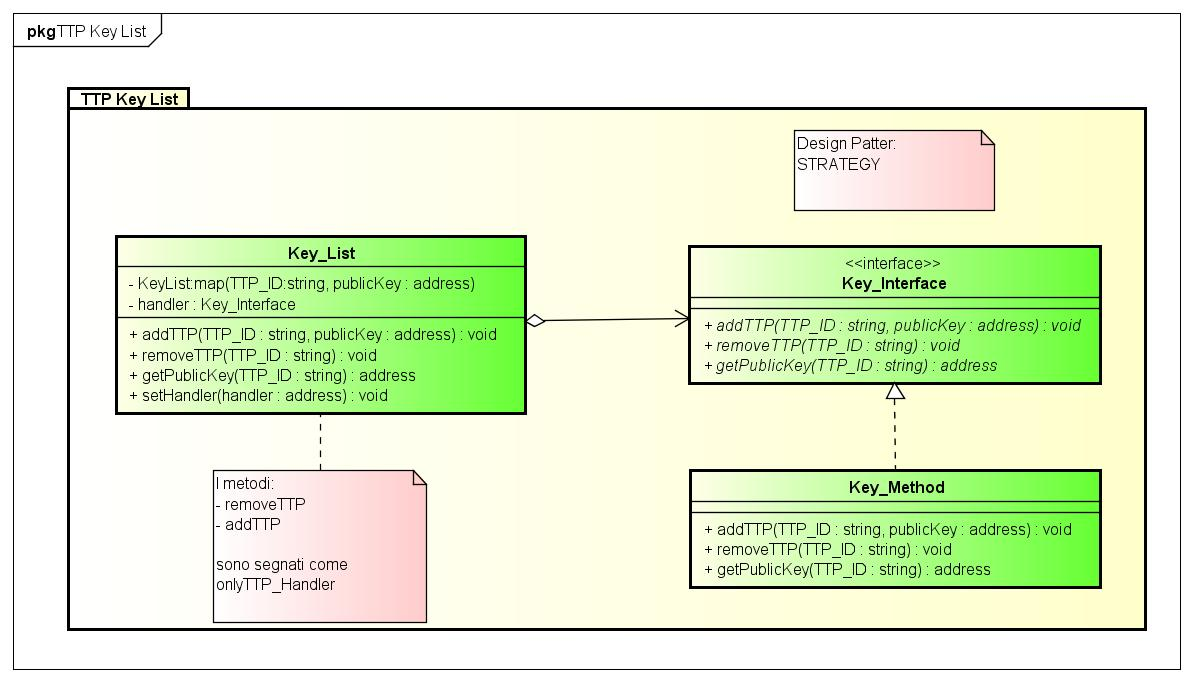
\includegraphics[width=0.8\textwidth]{immagini/ttpkeylist}
	\caption{Schema TTP Key List}
\end{figure}
\begin{itemize}
	\item \textbf{Descrizione}
	Questa componente fa da tramite tra il Service Provider Handler e Trusted Third Party Handler.
	Ogni qual volta un Service Provider vuole recuperare le informazioni di un utente e vuole verificare che, contenute nel suo oggetto Identity, siano certificate recupera, tramite TTP Key List, la chiave pubblica dell'ente certificatore che ha certificato le informazioni dell'utente e, tramite un confronto con la firma posta nelle informazioni personali dell'utente (firma = hash(dati utente + chiave privata \gls{TTP})), controlla che le informazioni siano effettivamente state firmate dall'ente che è stato segnato come certificatore per quelle informazioni.\\
	Quindi, questa componente, è di fondamentale importanza per permettere il sistema di verifica e certificazione che il modulo \gls{ITF} deve implementare.\\
	Anche questa componente, come tutte le altre, viene implementata tramite uno \textit{strategy} pattern in modo da mantenere separata la logica e i dati che rappresentano l'associazione \gls{TTP} - chiave pubblica.\\
	Oltre a questo
	\item \textbf{Interazione con altre componenti}
	\begin{itemize}
		\item Service Provider Handler;
		\item Trusted Third Party Handler.
	\end{itemize}
	\item \textbf{Design pattern presenti}\\
	All'interno del package TTP Key List troviamo il design pattern \textit{strategy} ed è un \textit{singleton} per recuperare tutte le informazioni riguardanti gli enti certificatori autorizzati.
\end{itemize}
\subsubsection{Key\_List}
\begin{itemize}
	\item \textbf{Descrizione}
	Componente che gestisce tutto il package TTP Key List in quanto contiene sia i dati che i metodi necessari per recuperare tutte le informazioni necessarie per andare a verificare le informazioni personali dell'utente.\\
	La parte principale di questa componente sono principalmente i dati che rappresentano l'associazione tra l'identificativo univoco di un ente certificatore e la sua chiave pubblica necessaria per andare a verificare i dati.\\
	Insieme a questo contiene tutti i metodi, segnati come onlyTTP\_Handler, che servono per andare ad inserire, rimuovere e recuperare tutte le informazioni riguardo una Trusted Third Party.\\
	Come le altre componenti, anche questa delega l'implementazione dei metodi ad una componente terza il Key\_Method.
	\item \textbf{Interazione con altre componenti}
	\begin{itemize}
		\item \textbf{Key\_Interface}: Interfaccia che espone tutti i metodi necessari a Key\_List per poter recuperare, inserire e rimuovere le informazioni relative alle Trusted Third Party che certificano le informazioni personali degli utenti.\\
		È una delle componenti necessarie per andare a realizzare il design pattern I del package TTP Key List che separa dati da business logic.
		\item \textbf{Key\_Method} :Classe che realizza i metodi esposti dall'interfaccia Key\_Interface e che sono richiamati dalla classe Key\_List per implementare la business logic del package TTP Key List.
	\end{itemize}
	\item \textbf{Design pattern presenti}\\
	Componente che partecipa alla realizzazione del design pattern \textit{strategy} ed è un \textit{singleton} per recuperare tutte le informazioni riguardanti gli enti certificatori autorizzati.
\end{itemize}
\subsection{Trusted Third Party Handler}
\begin{figure}[!h]
	\centering
	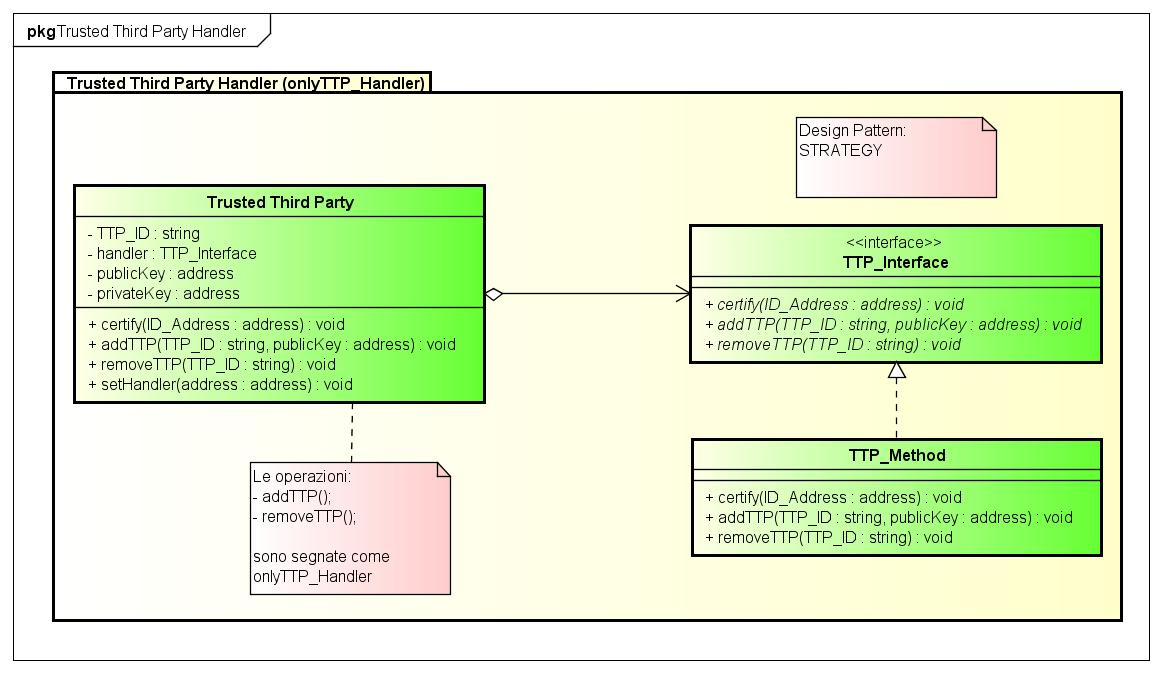
\includegraphics[width=0.8\textwidth]{immagini/trustedThirdPartyScheme}
	\caption{Schema Trusted Third Party}
\end{figure}
\begin{itemize}
	\item \textbf{Descrizione}
	Questa componente è necessaria per realizzare il pattern \textit{Observer} necessario per il funzionamento dell'intero sistema.\\
	La \gls{TTP} viene inserita all'interno di questo pattern in quanto, ogni qual volta un utente inserisce una nuova certificazione o un'informazione personale, in automatico viene notificata la Trusted Third Party.\\
	Questa, grazie all'indirizzo che gli viene passato dall'Identity Wallet Handler, recupera tutte le informazioni riguardanti l'identità di quell'utente e certifica le informazioni personali, appena aggiunte, ponendo la propria firma.\\
	Alcuni metodi di questo package come l'aggiunta e la rimozione di un ente certificatore dal sistema, sono segnati come onlyTTP\_Handler grazie alla funzionalità di proprietà di \textit{Solidity} che impedisce l'invocazione di metodi all'infuori del proprietario del contratto.
	\item \textbf{Interazione con altre componenti}
	\begin{itemize}
		\item Identity Wallet Handler;
		\item TTP Key List;
		\item Identity.
	\end{itemize}
	\item \textbf{Design pattern presenti}\\
	Seconda componente necessaria per la ralizzazione del pattern \textit{Observer}.
\end{itemize}
\subsubsection{Trusted Third Party}
\begin{itemize}
	\item \textbf{Descrizione}
	Componente interna al package Trusted Third Party Handler che ha lo scopo di mantenere al suo interno tutte le informazioni necessarie per poter certificare tutte le informazioni e certificazioni personali dell'utente.\\
	Contiene sia dati che invocazioni a metodi.\\
	I dati qui contenuti rappresentano, in modo univoco, l'ente certificatore (ID e Public Key) e il modo tramite la quale riesce a certificare i dati utente (Private Key).\\
	Per mantenere separata la \textit{business logic} dai dati partecipa come componente ad uno strategy pattern.
	\item \textbf{Interazione con altre componenti}
	\begin{itemize}
		\item \textbf{TTP\_Interface}: Interfaccia che contiene la firma dei metodi che il pattern \textit{strategy} deve realizzare all'interno del package Trusted Third Party Handler.\\
		Contiene tutti i metodi realizzati da TTP\_Method e richiamati da Trusted Third Party.		
		\item \textbf{TTP\_Method}: Componente concreta che realizza i metodi esposti dall'interfaccia TTP\_Interface e richiamati dal componente Trusted Third Party.\\
		Questa componente è fondamentale per andare a realizzare il design pattern \textit{strategy} che troviamo all'interno del package Trusted Third Party Handler
	\end{itemize}
	\item \textbf{Design pattern presenti}\\
	Partecipa alla realizzazione del design pattern \textit{strategy} interno al package.
\end{itemize}
\newpage
\subsection{Service Provider Handler}
\begin{figure}[!h]
	\centering
	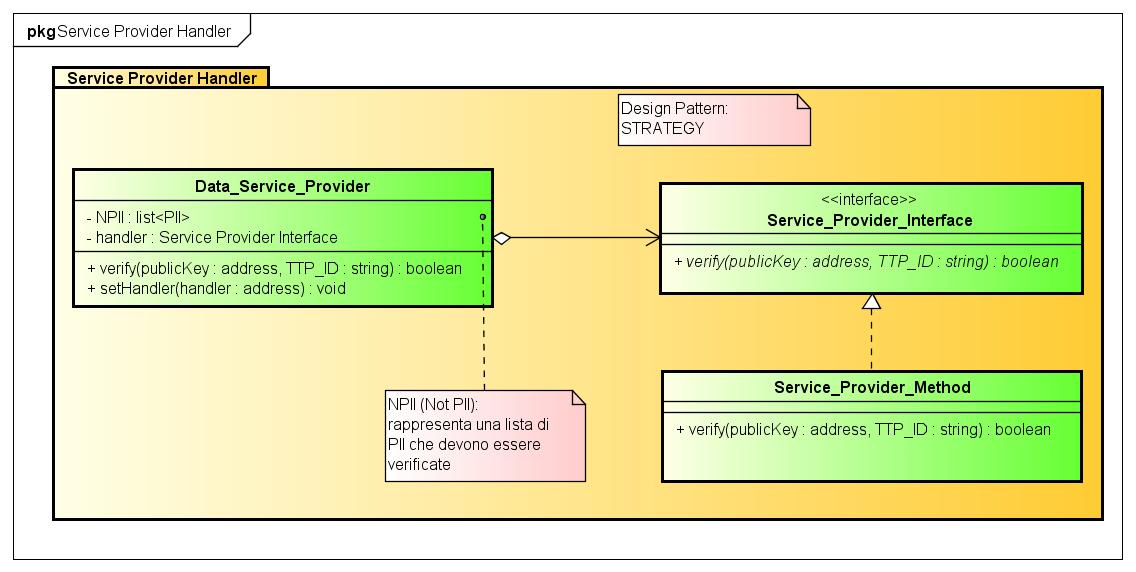
\includegraphics[width=0.8\textwidth]{immagini/serviceproviderhandler}
	\caption{Schema Service Provider}
\end{figure}
\begin{itemize}
	\item \textbf{Descrizione}
	Questo package è modella tutte le interazioni che avvengono tra il mondo esterno e la \textit{Blockchain Ethereum} che modella il sistema \gls{ITF}. In particolare modella tutte le operazioni che un Service Provider deve effettuare prima di erogare i suoi servizi ad un particolare utente.\\
	Per questo motivo, oltre che il consueto \textit{strategy} pattern questo package implementa anche il design pattern \textit{façade} per permettere l'interazione tra il presentation layer lato Serivce Provider e il sistema interno alla \textit{Blockchain Ethereum}.\\
	L'operazione principale che viene effettuata da questi componenti è la verifica delle informazioni personali di un utente (\gls{PII}) per accertarsi che siano certificate (firmate da un ente certificatore fidato).
	\item \textbf{Interazione con altre componenti}
	\begin{itemize}
		\item ID List;
		\item Identity;
		\item TTP Key List.
	\end{itemize}
	\item \textbf{Design pattern presenti}\\
	Oltre al consueto pattern \textit{strategy} questo contratto funge anche da \textit{façade} tra l'\gls{ITF} e il mondo esterno dalla parte di un Service Provider.
\end{itemize}
\subsubsection{Data\_Service\_Provider}
\begin{itemize}
	\item \textbf{Descrizione}
	\item \textbf{Interazione con altre componenti}
	\begin{itemize}
		\item Service\_Provider\_Interface:Interfaccia che espone tutti i metodi necessari a Data\_Service\_Provider per poter implementare le funzionalità di verifica richieste dal Service Provider prima di erogare i servizi ad un utente.
		\item Service\_Provider\_Method:Classe concreta che implementa tutti i metodi esposti da Data\_Service\_Interface e che sono necessari a Data\_Service\_Provider per poter implementare la business logic del package Service Provider Handler.
	\end{itemize}
	\item \textbf{Design Pattern presenti}\\
	Componente necessaria per implementare il design pattern \textit{strategy}.
\end{itemize}
\section{Design Pattern}
In questa sezione vengono descritti i design pattern utilizzati per la realizzazione del prodotto. I design pattern sono delle soluzioni progettuali generali a problemi ricorrenti che possono essere adottati durante lo sviluppo del proprio sistema.
\subsection{Singleton}
\begin{itemize}
	\item \textbf{Scopo di utilizzo}: il pattern Singleton assicura che una certa classe abbia una sola istanza e fornisce ad essa un punto d’acceso globale.
	\item \textbf{Contesto}: all'interno dell’applicazione questo pattern viene usato per garantire la presenza di un unica istanza dei contratti TTP Key List e ID List.
\end{itemize}
\subsection{Façade}
\begin{itemize}
	\item \textbf{Scopo di utilizzo}: consente di definire un'interfaccia ad alto livello che semplifica l'accesso alle funzionalità erogate dal sottosistema e che fornisce un entry-point unico al sottosistema stesso;
	\item \textbf{Contesto}: per la realizzazione del modulo \gls{ITF} l'utilizzo di un design pattern di questo tipo è necessario in quanto bisogna far sì che l'utente riesca ad interagire con la \textit{Blockchain Ethereum} senza che si preoccupi della complessità del sistema e delle logiche che governano questo tipo di tecnologia come la gestione degli \emph{\gls{ether}}\glsfirstoccur, del \emph{\gls{gas}}\glsfirstoccur, spesa degli \gls{ether} per le transazioni.
\end{itemize}
\subsection{Strategy}
\begin{itemize}
	\item \textbf{Scopo di utilizzo}: Il pattern Strategy permette di definire una famiglia di algoritmi, di incapsularli e renderli intercambiabili fra loro. Questo pattern consente agli algoritmi di variare in modo indipendente rispetto al loro contesto di utilizzo, fornendo un basso accoppiamento tra le classi partecipanti.
	\item \textbf{Contesto}: la motivazione che ha portato alla scelta di questo pattern, è il fatto che, ogni qual volta qualcosa viene inserito all'interno della rete \textit{Blockchain Ethereum} diventa immutabile.\\
	Per questo motivo si è deciso di strutturare tutto il sistema in package che, al loro interno, dividessero i dati dall'implementazione dei metodi.\\
	Questo viene fatto perché se un metodo contiene errori o comportamenti anomali, sarebbe necessario sostituire tutto il contratto, perdendo anche tutti i dati utente fino ad ora accumulati.\\
	Tramite pattern Strategy e alle funzionalità di \textit{Solidity} è possibile separare queste due componenti e, tramite indirizzi, far sì che sia una componente terza a implementare concretamente i metodi.
	In caso di errori o comportamenti anomali è sufficiente creare un nuovo contratto da aggiungere alle componenti che ereditano dall'interfaccia che realizza lo Strategy e far sì che sia questa nuova componente ad eseguire i metodi che vengono chiamati	
\end{itemize}
\subsection{Observer}
\begin{itemize}
	\item \textbf{Scopo di utilizzo}: Il pattern Observer permette di definire una dipendeza uno a molti fra oggetti, in modo tale che se un oggetto cambia il suo stato interno, ciascuno degli oggetti dipendenti da esso viene notificato e aggiornato automaticamente.
	\item \textbf{Contesto}: All'interno del modulo \gls{ITF} questa tipologia di design pattern è richiesta nel momento in cui un utente si registra ed inserisce, o aggiorna, le sue \gls{PII}.\\
	In automatico, un oggetto \gls{TTP}, deve essere notificato del fatto che è avvenuta l'aggiunta di nuove informazioni così da poterle certificare per essere utilizzate da un Service Provider quando vuole erogare un servizio ad un utente che lo richiede.
\end{itemize}             % Concept Preview
% !TEX encoding = UTF-8
% !TEX TS-program = pdflatex
% !TEX root = ../tesi.tex

%**************************************************************
\chapter{Codifica}
\label{cap:codifica}
%**************************************************************
Dopo aver analizato l'architettura del modulo \gls{ITF} insieme ai design pattern necessari alla realizzazione del prodotto passiamo ad analizzare nel dettaglio la struttura delle singole componenti.\\
I seguenti paragrafi analizzano quali metodi, attributi ed eventuali sottoclassi compongono i package più importanti necessari per la realizzazione del sistema.\\
Andremo ad analizzare:
\begin{itemize}
	\item \textbf{Data\_Identity\_Wallet} contenuto nel package \textit{Identity Wallet Handler};
	\item \textbf{Trusted Third Party} contenuto nel package \textit{Trusted Third Party Handler};
	\item \textbf{Data\_ID\_List} contenuto nel package \textit{ID List};
	\item \textbf{Data\_Identity} contenuto nel package \textit{Identity};
	\item \textbf{Personally Identifiable Information};
	\item \textbf{Key\_List} contenuto nel package \textit{TTP Key List};
	\item \textbf{Data\_Service\_Provider}contenuto nel package \textit{Service Provider Handler}.
\end{itemize}
\newpage
\section{Identity Wallet Handler}
\subsection{Data\_Identity\_Wallet}
\begin{figure}[h]
	\centering
	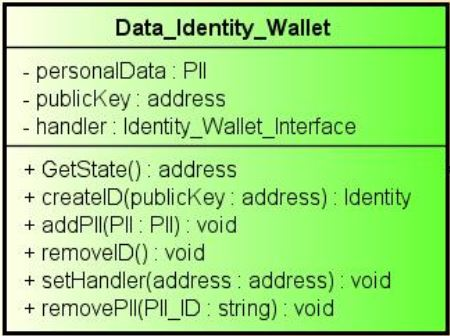
\includegraphics[width=0.5\textwidth]{immagini/identitywalletdata}
	\caption{Schema Data Identity Wallet}
\end{figure}
\begin{itemize}
	\item \textbf{Descrizione}\\
	Classe concreta utilizzata per modellare tutte le operazioni che un utente può effettuare con il sistema \gls{ITF}.
	\item \textbf{Attributi}
	\begin{itemize}
		\item \textit{- personalData: PII}\\
		Contiene le \gls{PII} che un utente ha inserito tramite l'applicativo e che vuole inserire nel proprio profilo;
		\item \textit{- publicKey: address}\\
		Chiave pubblica univoca che rappresenta l'identità di un utente all'interno del sistema \gls{ITF};
		\item \textit{- handler: Identity\_Wallet\_Interface}\\
		Oggetto necessario per l'implementazione del pattern \textit{strategy}. Tramite questo oggetto verranno invocati i metodi del modulo.
	\end{itemize}
	\item \textbf{Metodi}
	\begin{itemize}
		\item \textit{+ GetState(): void}\\
		Metodo necessario per realizzare il patterno \textit{observer} per la certificazione automatica delle \gls{PII}.
		\item \textit{+ createID(publicKey: address): identity}\\
		Metodo che permette la creazione di una nuova identità digitale all'interno del modulo \gls{ITF}.
		\textbf{Parametri:}
		\begin{itemize}
			\item \textit{publicKey: address}\\
			Chiave pubblica dell'identità che si vuole creare. Questo parametro è necessario per permettere l'associazione \textit{publicKey - indirizzo} in modo da andare a recuperare l'identità a partire dalla chiave pubblica.
		\end{itemize}
		\item \textit{+ addPII(PII: PII): void}\\
		Metodo necessario per aggiungere una o più nuove informazioni personali all'identità utente.\\\\
		\textbf{Parametri:}
		\begin{itemize}
			\item \textit{PII: PII}\\
			Informazioni personali che l'utente vuole inserire all'interno della propria identità digitale.
		\end{itemize}
		\item \textit{+ removeID(): void}\\
		Metodo che rimuove l'identità digitale dell'utente del sistema andando a cancellare la sua entry nella struttura dati che associa le chiavi pubbliche agli indirizzi delle identità.
		\item \textit{+ setHandler(address: address): void}\\
		Metodo necessario per impostare l'indirizzo dell'oggetto che deve andare ad implementare i medtodi. Il metodo è segnato come pubblico anche se, grazie a \textit{Solidity}, bisogna impostare la proprietà dell'oggetto in modo che solo il proprietario del contratto possa cambiare l'indirizzo dell'oggetto che risolve i metodi.\\\\
		\textbf{Parametri:}
		\begin{itemize}
			\item \textit{address: address}
			Indirizzo dell'oggetto delegato alla risoluzione dei metodi.
		\end{itemize}
		\item \textit{+ removePII(PII\_ID: string): void}\\
		Metodo che permette ad un utente di rimuovere una o più informazoni personali che sono state inserite e certificate all'interno della propria identità digitale.\\\\
		\textbf{Parametri:}
		\begin{itemize}
			\item \textit{PII\_ID: string}\\
			Rappresenta l'identificativo univoco che va ad identificare l'informazione personale che si desidera rimuovere.
		\end{itemize}
	\end{itemize}
\end{itemize}
\section{Trusted Third Party Handler}
\subsection{Trusted Third Party}
\begin{figure}[!h]
	\centering
	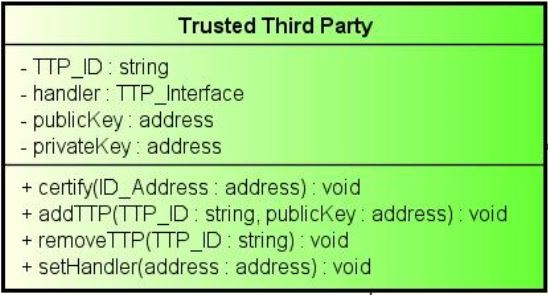
\includegraphics[width=0.5\textwidth]{immagini/ttpData}
	\caption{Schema Trusted Third Party}
\end{figure}
\begin{itemize}
	\item \textbf{Descrizione}\\
	Classe concreta utilizzata per modellare tutte le operazioni che un ente certificatore può fare sulle \gls{PII} di un utente ogni qual volta queste vengono aggiunte.\\
	Son presenti anche funzionalità per aggiungere e rimuovere nuovi enti certificatori.
	\item \textbf{Attributi}
	\begin{itemize}
		\item \textit{- TT\_ID: string}\\
		Rappresenta l'identificativo univoco mnemonico che identifica un ente certificatore.
		\item \textit{- handler: TTP\_Interface}\\
		Indirizzo dell'oggetto concreto che va a realizzare i metodi della classe, ponendo quindi fine alla catena di deleghe.
		\item \textit{- publicKey: address}\\
		Chiave pubblica utilizzata per permettere la decodifica, da parte del Service Provider Handler, del \textit{hash} per permettere la verifica.
		\item \textit{- privateKey: address}\\
		Chiave privata dell'ente certificatore necessaria epr andare a certificare le informazioni personali dell'utente.
	\end{itemize}
	\item \textbf{Metodi}
	\begin{itemize}
		\item \textit{+ certify(ID\_Address: address): void}\\
		Metodo principale della classe Trusted Third Party. Compie la funzione, fondamentale, di andare a certificare le informazioni personali che un utente inserisce all'interno della sua identità digitale. Questa azione viene scatenata in automatico quando un utente aggiorna o inserisce nuove \gls{PII} grazie al pattern \textit{observer}.\\\\
		\textbf{Parametri:}
		\begin{itemize}
			\item \textit{ID\_Address: address}\\
			Indirizzo dell'oggetto Identity che rappresenta l'identità dell'utente che ha aggiunto una nuova \gls{PII}. Questo indirizzo è necessario per poter recuperare le informazioni personali aggiunte e per poterle certificare.			
		\end{itemize}
		\item \textit{+ addTTP(TTP\_ID: string, publicKey: address): void}\\
		Metodo che permettere di aggiungere un nuovo ente certificatore alla lista di enti che possono certificare le informazioni personali degli utenti. L'aggiunta avviene associando l'identificativo mnemonico con la chiave pubblica necessaria per l'attività di verifica delle informazioni certificate.\\\\
		\textbf{Parametri:}
		\begin{itemize}
			\item \textit{TTP\_ID: string}\\
			Identificativo univoco mnemonico che rappresenta un ente certificatore;
			\item \textit{publicKey: address}\\
			Chiave pubblica dell'ente certificatore necessaria per l'attività di verifica delle informazioni certificate.
		\end{itemize}
		\item \textit{+ removeTTP(TTP\_ID: string): void}\\
		Metodo necessario per poter rimuovere un ente certificatore dalla lista di quelli che possono certificare le informazioni degli utenti.\\\\
		\textbf{Parametri:}
		\begin{itemize}
			\item \textit{TTP\_ID: string}\\
			Identificativo univoco mnemonico necessario per sepcificare quale ente certificatore si vuole rimuovere dalla lista.
		\end{itemize}
		\item \textit{+ setHandler(address: address): void}\\
		Metodo necessario per impostare l'indirizzo dell'oggetto che deve andare ad implementare i medtodi. Il metodo è segnato come pubblico anche se, grazie a \textit{Solidity}, bisogna impostare la proprietà dell'oggetto in modo che solo il proprietario del contratto possa cambiare l'indirizzo dell'oggetto che risolve i metodi.\\\\
		\textbf{Parametri:}
		\begin{itemize}
			\item \textit{address: address}\\
			Indirizzo dell'oggetto delegato alla risoluzione dei metodi.
		\end{itemize}
	\end{itemize}
\end{itemize}
\section{ID List}
\subsection{Data\_ID\_List}
\begin{figure}[!h]
	\centering
	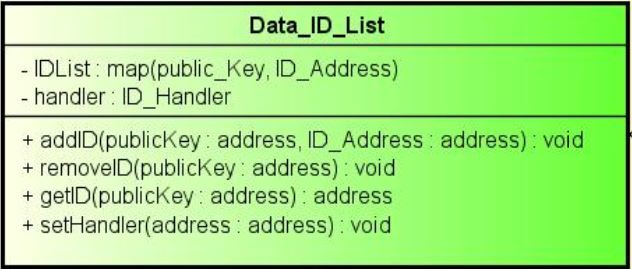
\includegraphics[width=0.5\textwidth]{immagini/dataIDList}
	\caption{Schema Data Identity List}
\end{figure}
\begin{itemize}
	\item \textbf{Descrizione}\\
	Classe concreta utilizzata per accoppiare l'identità di un utente (rappresentata dalla sua chiave pubblica) e le sue informazioni personali contenute nel proprio oggetto Identity.
	\item \textbf{Attributi}
	\begin{itemize}
		\item \textit{- IDList: map(publicKey, ID\_Address)}\\
		Componente fondamentale dell'intero package. Associa una chiave pubblica di tipo \textit{address} con l'indirizzo, sempre di tipo \textit{address}, associato all'oggetto identity che rappresenta le \gls{PII} dell'utente rappresentato dalla chiave pubblica inserita.\\
		Grazie a questa mappa è possibile, per ogni utente, recuperare le \gls{PII} a lui associate.
		\item \textit{- handler: ID\_Handler}\\
		Indirizzo dell'oggetto concreto che va a realizzare i metodi della classe, ponendo fine alla catena di deleghe.		
	\end{itemize}
	\item \textbf{Metodi}
	\begin{itemize}
		\item \textit{+ addID(publicKey: address, ID\_Address: address): void}\\
		Metodo che consente di aggiungere una nuova associazione utente-identità all'interno della mappa.\\\\
		\textbf{Parametri:}
		\begin{itemize}
			\item \textit{publicKey: address}\\
			Chiave pubblica associata all'utente che rappresenta il suo identificativo univoco;
			\item \textit{ID\_Address: address}\\
			Indirizzo \textit{Ethereum} che rappresenta un "puntatore" grazie al quale è possibile rcuperare le \gls{PII} di un utente.
		\end{itemize}
		\item \textit{+ removeID(publicKey: address): void}\\
		Metodo che consente di rimuovere dalla mappa un'associazione utente-identità. In questo modo è possibile rendere irrecuperabile tutte le informazioni riguardanti un utente nel caso in cui questo decida di eliminare il proprio profilo dal sistema \gls{ITF}.\\\\
		\textbf{Parametri:}
		\begin{itemize}
			\item \textit{publicKey: address}\\
			Chiave pubblica (identificativo univoco) dell'utente della quale si vuole eliminare l'identità.
		\end{itemize}
		\item \textit{+ getID(publicKey: address): address}\\
		Metodo che consente di recuperare l'indirizzo dove trovare le informazioni personali dell'utente passato come parametro (tramite chiave pubblica).\\\\
		\textbf{Parametri:}
		\begin{itemize}
			\item \textit{publicKey: address}\\
			Chiave pubblica dell'utente della quale si vogliono recuperare le \gls{PII} per andare a verificare le sue informazioni.
		\end{itemize}
		\item \textit{+ setHandler(address: address): void}\\
		Metodo necessario per impostare l'indirizzo dell'oggetto che deve andare ad implementare i medtodi. Il metodo è segnato come pubblico anche se, grazie a \textit{Solidity}, bisogna impostare la proprietà dell'oggetto in modo che solo il proprietario del contratto possa cambiare l'indirizzo dell'oggetto che risolve i metodi.\\\\
		\textbf{Parametri:}
		\begin{itemize}
			\item \textit{address: address}\\
			Indirizzo dell'oggetto delegato alla risoluzione dei metodi.
		\end{itemize}
	\end{itemize}
\end{itemize}
\newpage
\section{Identity}
\subsection{Data\_Identity}
\begin{figure}[!h]
	\centering
	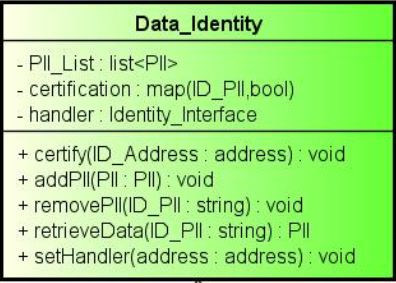
\includegraphics[width=0.5\textwidth]{immagini/identityData}
	\caption{Schema Data Identity}
\end{figure}
\begin{itemize}
	\item \textbf{Descrizione}\\
	Classe concreta utilizzata all'interno del sistema \gls{ITF} per rappresentare e manipolare l'identità di un utente.
	\item \textbf{Attributi}
	\begin{itemize}
		\item \textit{- PII\_List: list<PII>}\\
		Lista che contiene tutte le informazioni personali certificate associate ad un utente.
		\item \textit{- certification: map<ID\_PII. bool>}\\
		Mappa che, per ogni \gls{PII} presente nella lista, tiene traccia di quali sono certificate e quali no.
		\item \textit{- handler: Identity\_Interface}\\
		Indirizzo dell'oggetto concreto che va a realizzare i metodi della classe, ponendo quindi fine alla catena di deleghe.
	\end{itemize}
	\item \textbf{Metodi}
	\begin{itemize}
		\item \textit{+certify(ID\_Address: address): void}\\
		Metodo necessario all'ente certificatore per poter certificare tutte le informazioni personali che l'utente inserisce.\\\\
		\textbf{Parametri:}
		\begin{itemize}
			\item \textit{ID\_Address: address}\\
			Indirizzo delle informazioni personali da certificare.
		\end{itemize}
		\item \textit{+ addPII(PII: PII): void}\\
		Metodo utilizzato per aggiungere un'informazione eprsnale all'interno della lsita delle \gls{PII} associate all'utente.\\\\
		\textbf{Parametri:}
		\begin{itemize}
			\item \textit{PII: PII}\\
			Oggetto che rappresenta l'informazione personale che si vuole inserire e associare all'utente.
		\end{itemize}
		\item \textit{+ removePII(ID\_PII: string): void}\\
		Rimuove un'informazione personale dalla lista delle \gls{PII} associate all'utente.\\\\
		\textbf{Parametri:}
		\begin{itemize}
			\item \textit{ID\_PII: string}\\
			Identificativo univoco per identificare quale delle informazioni personali dell'utente si vuole rimuovere dalla sua lista.
		\end{itemize}
		\item \textit{+ retrieveData(ID\_PII: string): PII}\\
		Metodo utilizzato per recuperare tutto l'oggetto che rappresenta l'informazione personale dell'utente.\\\\
		\textbf{Parametri:}
		\begin{itemize}
			\item \textit{ID\_PII: string}\\
			Identificativo univoco mnemonico utilizzato per indicare quale delle informazioni personali recuperare dalla lista.
		\end{itemize}
		\item \textit{+ setHandler(address: address): void}\\
		Metodo necessario per impostare l'indirizzo dell'oggetto che deve andare ad implementare i medtodi. Il metodo è segnato come pubblico anche se, grazie a \textit{Solidity}, bisogna impostare la proprietà dell'oggetto in modo che solo il proprietario del contratto possa cambiare l'indirizzo dell'oggetto che risolve i metodi.\\\\
		\textbf{Parametri:}
		\begin{itemize}
			\item \textit{address: address}\\
			Indirizzo dell'oggetto delegato alla risoluzione dei metodi.
		\end{itemize}
	\end{itemize}
\end{itemize}
\section{Personally Identifiable Information}
\begin{figure}[!h]
	\centering
	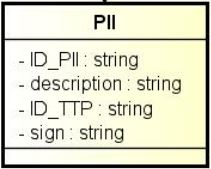
\includegraphics[width=0.5\textwidth]{immagini/pii}
	\caption{Schema Personally Identifiable Information}
\end{figure}
\begin{itemize}
	\item \textbf{Descrizione}\\
	Classe concreta necessaria che rappresenta un informazione eprsonale dell'utente all'interno del sistema \gls{ITF}.
	\item \textbf{Attributi}\\
	\begin{itemize}
		\item \textit{- ID\_PII: string}\\
		Identificativo univoco mnemonico necessario per individuare facilmente la \gls{PII}.
		\item \textit{- description: string}\\
		Campo che descrive il tipo di informazione personale.
		\item \textit{- ID\_TTP: string}\\
		Identificativo univoco mnemonico che rappresenta l'ente certificatore che ha certificato, tramite firma, la \gls{PII}.
		\item \textit{- sign: string}\\
		Firma che certifica la \gls{PII}. Questa firma è ottenuta dall'\textit{hash} dei dati uniti alla chiave privata dell'ente certificatore che vuole certificarli.
	\end{itemize}
\end{itemize}
\section{TTP Key List}
\subsection{Key\_List}
\begin{figure}[!h]
	\centering
	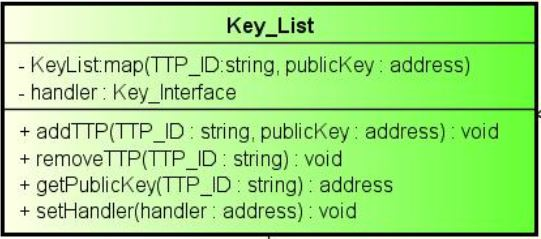
\includegraphics[width=0.5\textwidth]{immagini/keylistData}
	\caption{Schema Key List}
\end{figure}
\begin{itemize}
	\item \textbf{Descrizione}\\
	Classe concreta che mantiene una mappa che consente di associare un identificativo mnemonico, che rappresenta un ente certificatore, e la sua chiave pubblica necessara per poter verificare le \gls{PII} certificate.
	\item \textbf{Attributi}
	\begin{itemize}
		\item \textit{- KeyList: map<TTP\_ID: string, publicKey: address>}\\
		Mappa che mantiene tutte le associazioni tra identificativo univoco mnemonico e rispettive chiavi pubbliche.\\
		Questa lista è necessaria per poter recuperare, dato l'ID della \gls{TTP}, la chiave pubblica per la successiva verifica delle informazioni personali dell'utente.
		\item \textit{- handler: key\_interface}\\
		Indirizzo dell'oggetto concreto che va a realizzare i metodi della classe, ponendo quindi fine alla catena di deleghe.		
	\end{itemize}
	\item \textbf{Metodi}
	\begin{itemize}
		\item \textit{+ addTTP(TTP\_ID: string, publicKey: address): void}\\
		Metodo pensato per poter espandere la lista di enti certificatori che possono certificare le informazioni personali contenute nel sistema.\\\\
		\textbf{Parametri:}
		\begin{itemize}
			\item \textit{TTP\_ID: string}\\
			Identificativo univoco mnemonico necessario per permettere l'associazione delle informazioni;
			\item \textit{publicKey: address}\\
			Chiave pubblica dell'ente certificatore che si desidera agiungere alla mappa.
		\end{itemize}
		\item \textit{+ removeTTP(TTP\_ID: string): void}\\
		Metodo che consente di rimuovere gli enti certificatori dalla lista di quelli idonei a certificare le \gls{PII} delgi utenti.\\\\
		\textbf{Parametri:}
		\begin{itemize}
			\item \textit{TTP\_ID: string}\\
			Identificativo univoco mnemonico dell'ente certificatore che si desidera rimuovere dalla lista degli enti idonei alla certificazione.
		\end{itemize}
		\item \textit{+ getPublicKey(TTP\_ID: string): address}\\
		Metodo che consente di recuperare la chiave pubblica a partire dall'identificativo univoco mnemonico dell'ente certificatore.\\\\
		\textbf{Parametri:}
		\begin{itemize}
			\item \textit{TTP\_ID: string}\\
			Identificativo univoco mnemonico dell'ente certificatore della quale si desidera recuperare la chiave pubblica.
		\end{itemize}
		\item \textit{+ setHandler(address: address): void}\\
		Metodo necessario per impostare l'indirizzo dell'oggetto che deve andare ad implementare i medtodi. Il metodo è segnato come pubblico anche se, grazie a \textit{Solidity}, bisogna impostare la proprietà dell'oggetto in modo che solo il proprietario del contratto possa cambiare l'indirizzo dell'oggetto che risolve i metodi.\\\\
		\textbf{Parametri:}
		\begin{itemize}
			\item \textit{address: address}\\
			Indirizzo dell'oggetto delegato alla risoluzione dei metodi.
		\end{itemize}
	\end{itemize}
\end{itemize}
\newpage
\section{Service Provider Handler}
\subsection{Data\_Service\_Provider}
\begin{figure}[!h]
	\centering
	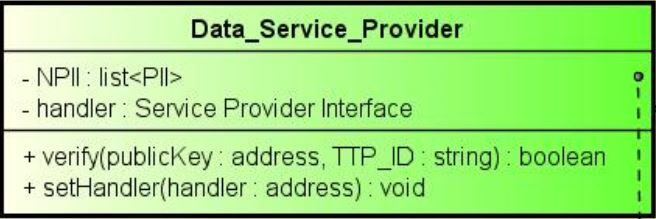
\includegraphics[width=0.5\textwidth]{immagini/dataSP}
	\caption{Schema Data Service Provider}
\end{figure}
\begin{itemize}
	\item \textbf{Descrizione}\\
	Classe concreta utilizzata per manipolare tutte le informazioni personali che il serivce provider deve verificare prima di permettere l'accesso e l'erogazione di servizi all'utente che li ha richiesti.
	\item \textbf{Attributi}
	\begin{itemize}
		\item \textit{- NPII: list<PII>}\\
		\textit{Not PII} nome dato alla lista delle \gls{PII} che il service provider richiede siano verificate per poter rilasciare il servizio all'utente che li ha richiesti.
		\item \textit{- handler: Service\_Provider\_Interface}\\
		Indirizzo dell'oggetto concreto che va a realizzare i metodi della classe ponendo fine alla catena di deleghe.
	\end{itemize}
	\item \textbf{Metodi}
	\begin{itemize}
		\item \textit{+ verify(publicKey: address, TTP\_ID:string): boolean}\\
		Metodo fondamentale del package che consente la verifica delle informazioni personali dell'utente passato come parametro (identificato tramite la sua chiave pubblica).\\
		Dalla chiave pubblica, utilizzando ID List, è possibile recuperare le \gls{PII} associate all'utente e verificare che siano certificate.\\
		La verifica avviene tramite confronto dell'\textit{hash} nel \gls{PII} con il nuovo \textit{hash} calcolato a partire dai dati e la chiave pubblica del \gls{TTP}.\\
		La chiave pubblica del \gls{TTP} viene recuperata tramite TTP\_ID utilizzando il package TTP Key List.\\\\
		\textbf{Parametri:}
		\begin{itemize}
			\item \textit{publicKey: address}\\
			Chiave pubblica necessara per recuperare le \gls{PII} dell'utente che ha richiesto l'accesso ad un servizio;
			\item \textit{TTP\_ID: string}\\
			Identificativo univoco mnemonico dell'ente certificatore che ha certificato le informazioni personali. Questo attributo è utilizzato per recuperare la chiave pubblica necessaria per la verifica degli \textit{hash}.
		\end{itemize}
		\item \textit{+ setHandler(address: address): void}\\
		Metodo necessario per impostare l'indirizzo dell'oggetto che deve andare ad implementare i medtodi. Il metodo è segnato come pubblico anche se, grazie a \textit{Solidity}, bisogna impostare la proprietà dell'oggetto in modo che solo il proprietario del contratto possa cambiare l'indirizzo dell'oggetto che risolve i metodi.\\\\
		\textbf{Parametri:}
		\begin{itemize}
			\item \textit{address: address}\\
			Indirizzo dell'oggetto delegato alla risoluzione dei metodi.
		\end{itemize}		
	\end{itemize}
\end{itemize}
             % Product Prototype
% !TEX encoding = UTF-8
% !TEX TS-program = pdflatex
% !TEX root = ../tesi.tex

%**************************************************************
\chapter{Verifica e validazione}
\label{cap:verifica_validazione}
%**************************************************************             % Product Design Freeze e SOP
% !TEX encoding = UTF-8
% !TEX TS-program = pdflatex
% !TEX root = ../tesi.tex

%**************************************************************
\chapter{Valutazione finale}
\label{cap:valutazione_finale}
%**************************************************************
In questo capitolo viene fatto un \textit{excursus} riguardo gli obiettivi prefissati, il consuntivo orario finale in relazione al piano di lavoro concordato, le nuove conoscenze acquisite e, infine, una valutazione personale dello stage.
%**************************************************************
\section{Raggiungimento degli obiettivi}
Durante l'attività di stage qualche requisito riguardante le funzionalità ha subito, fermi restando gli obiettivi prefissati, dei leggeri cambiamenti in seguito a più approfonditi studi di dominio e della tecnologia \textit{Blockchain} scelta. Questo, fortunatamente, non ha avuto alcuna ripercussione sia dal punto di vista dei tempi stimanti che del raggiungimento degli obiettivi posti nel Piano di Lavoro.
\begin{longtable}{|r l|p{3cm}|p{8cm}|p{2cm}|}
	\hline
	\multicolumn{2}{|c|}{\textbf{ID}} & \textbf{IMPORTANZA} & \textbf{DESCRIZIONE} & \textbf{STATO}\tabularnewline
	\hline
	& O1 & Obbligatorio & Studio del dominio applicativo & Completato\\\hline
	& O2 & Obbligatorio & Studio delle possibili tecnologie \textit{Blockchain} da adottare & Completato \\\hline
	& O3 & Obbligatorio & Analisi comparativa delle tecnologie \textit{Blockchain} individuate & Completato \\\hline
	& O4 & Obbligatorio & Definizione dei vari casi d'uso per le funzionalità richieste (sopracitate) & Completato \\\hline
	& O4.1 & Obbligatorio & Definizione dei casi d'uso per la funzionalità di registrazione & Completato\\\hline
	& O4.2 & Obbligatorio & Definizione dei casi d'uso per a funzionalità di certificazione & Completato\\\hline
	& O4.3 & Obbligatorio & Definizione dei casi d'uso per la funzionalità di verifica & Completato\\\hline
	& O5 & Obbligatorio & Stesura del documento di analisi dei requisiti & Completato\\\hline
	& O6 & Obbligatorio & Stesura del documento contenete le specifiche architetturali del sistema & Completato\\\hline
	& O7 & Obbligatorio & Realizzazione del modulo \gls{ITF} & Completato\\\hline
	& O7.1 & Obbligatorio & Realizzazione della struttura e della gerarchia di classi necessaria alla realizzazione del modulo & Completato \\\hline
	& O7.2 & Obbligatorio & Implementazione dei metodi necessari per il corretto funzionamento del modulo & Completato\\\hline
	& D1 & Desiderabile & Produzione della documentazione relativa alle analisi svolte & Completato \\\hline
	& D2 & Desiderabile & Definizione dei casi d'uso per la funzionalità di presentazione dei dati & Completato \\\hline
	& D3 & Desiderabile & Definizione dei casi d'uso per la funzionalità di accesso al servizio & Completato\\\hline
	& D4 & Desiderabile & Stesura del documento di progettazione & Completato\\\hline
	& D5 & Desiderabile & Realizzazione dei test necessari alla verifica del corretto funzionamento del sistema & Completato\\\hline
	& D5.1 & Desiderabile & Implementazione dei test di unità per i singoli metodi & Completato\\\hline
	& D5.2 & Desiderabile & Implemetnazione dei test di integrazione per testare le classi & Completato\\\hline
	& D5.3 & Desiderabile & Implementazione dei test di integrazione per testare l'interazione tra tutte le classi che compongono il sistema & Completato\\\hline
	& F1 & Facoltativo & Stesura del documento relativo ai test di unità ed integrazione & Completato\\\hline	
	& F2 & Facoltativo & Stesura del documento relativo alla validazione del modulo (anomalie e bug) & Non completato\\\hline
	\caption{Tabella degli obiettivi raggiunti a fine stage}
\end{longtable}
Gli obiettivi la cui importanza era fondamentale per la realizzazione del modulo \gls{ITF} sono stati soddisfatti al 100\%.\\
Per quanto riguarda quelli desiderabili e facoltativi sono stati completati tutti tranne uno ovvero la\textit{ stesura del documento relativo alla validazione del modulo}. Questo perchè durante gli ultimi giorni di stage, in accordo con il tutor aziendale, si è preferito dare più importanza al \textit{testing} di tutto il modulo completo compresivo sia della mia parte che quella dell'altro stagista Simone Ballarin.
%**************************************************************
\section{Consuntivo finale}
Rispetto al piano di lavoro di inizio stage concordato con il tutor aziendale Sara Meneghetti e il responsabile di progetto Roberto Griggio, non ci sono state variazioni ai giorni di lavoro pianificate.\\
In conclusione, l'esperienza di stage ha avuto una durata complessiva di \textbf{320 ore} lavorative, come visibile in tabella, in cui viene riportata la fase lavorativa, già descritta nel paragrafo \hyperref[sec:pianificazione_del_lavoro]{pianificazione del lavoro} del \hyperref[cap:tecnologie_e_strumenti]{Capitolo 2}, le ore preventivate e le ore effettivamente svolte. 
\begin{longtable}{|r l|p{5cm}|p{4cm}|}
	\hline
	\multicolumn{2}{|c|}{\textbf{ATTIVITÀ}} & \textbf{ORE PREVENTIVATE} & \textbf{ORE EFFETTIVE}\tabularnewline
	\hline
	& Fase 1 & \centerline{40} & \centerline{40} \\\hline	
	& Fase 2 & \centerline{40} & \centerline{40}\\\hline
	& Fase 3 & \centerline{40} & \centerline{40}\\\hline
	& Fase 4 & \centerline{60} & \centerline{60}\\\hline
	& Fase 5 & \centerline{120} & \centerline{120}\\\hline
	& Fase 6 & \centerline{20} & \centerline{20}\\\hline	
	\caption{Riepilogo delle ore svolte durante lo stage}
\end{longtable}
%**************************************************************
\section{Conoscenze acquisite}
L'esperienza di stage vissuta mi ha permesso di ampliare le mie conoscenze sopratutto dal punto di vista tecnologico e organizzativo.\\
Ho imparato ad utilizzare moltissimi strumenti nuovi sopratutto per quanto riguarda il vasto mondo che circonda la tecnologia \textit{Blockchain} e le \gls{dapp} approfondendo ancora di più quanto già visto durante il progetto di Ingegneria del Software. Il dominio tecnologico che ho visto, analizzato, studiato e, in parte, utilizzato non era, quindi, una novità ma vedere le milioni di possibilità che offre è stato davvero entusiasmante e mi ha dato la voglia di approfondirlo ancora di più.
%**************************************************************
\section{Valutazione personale}
Personalmente ritengo questo stage un'esperienza fondamentale per la crescita professionale degli studenti.\\
Mi ha permesso di crescere molto sia a livello lavorativo che dei rapporti umani calati all'interno di un contesto totalmente diverso da quello che uno studente è, normalmente, abituato a vedere.\\
L'opportunità di stage che viene offerta dal nostro corso di studi è importantissima per la formazione che, un futuro neolaureato, deve avere prima di addentrarsi nel mondo lavorativo. Questo perchè ti da l'opportunità di acquisire capacità e attitudini che non vengono insegnate durante il corso di studi come il rispettare gli orari lavorativi imposti o la propensione positiva verso sfide nuove che, inizialmente, sono difficili e, apparentemente, fuori dalla portata dello studente.\\
Le conoscenze acquisite durante il corso di Laurea in Informatica sono state importantissime per la buona riuscita dello stage, non tanto dal punto di vista delle tecnologie studiate, ma dalla mentalità e capacità di ragionamento e adattamento che il corso di studi porta a maturare.\\
Bisogna dire che l'ambiente lavorativo è di fondamentale importanza per la buona riuscita dello stage e Athesys S.r.l è un luogo che mette subito a proprio agio gli studenti che si apprestano a questa nuova esperienza. Questo perchè è un ambiente giovane e rilassato in cui il personale è molto competente e non mette pressioni di fronte a difficoltà o ritardi anzi offre supporto e sprona a fare il proprio meglio.\\
Le 8 settimane di stage sono state, quindi, un esperienza altamente positiva che mi ha permesso di crescere molto anche dal punto di vista professionale grazie alla piena responsabilità, autonomia e fiducia che il responsabile, Roberto Griggio, mi ha dato per la realizzazione del progetto.             % Conclusioni
%**************************************************************
% Materiale finale
%**************************************************************
\backmatter
\printglossaries
% !TEX encoding = UTF-8
% !TEX TS-program = pdflatex
% !TEX root = ../tesi.tex

%**************************************************************
% Bibliografia
%**************************************************************

\cleardoublepage
\chapter{Bibliografia}

\nocite{*}
% Stampa i riferimenti bibliografici
\printbibliography[heading=subbibliography,title={Riferimenti bibliografici},type=book]

% Stampa i siti web consultati
\printbibliography[heading=subbibliography,title={Siti web consultati},type=online]


\end{document}
